%%%%%%%%%%%%%%%%%%%%%%%%%%%%%%%%%%%%%%%%%
% Beamer Presentation
% LaTeX Template
% Version 1.0 (10/11/12)
%
% This template has been downloaded from:
% http://www.LaTeXTemplates.com
%
% License:
% CC BY-NC-SA 3.0 (http://creativecommons.org/licenses/by-nc-sa/3.0/)
%
%%%%%%%%%%%%%%%%%%%%%%%%%%%%%%%%%%%%%%%%%

%----------------------------------------------------------------------------------------
%	PACKAGES AND THEMES
%----------------------------------------------------------------------------------------

\documentclass{beamer}

\mode<presentation> {

% The Beamer class comes with a number of default slide themes
% which change the colors and layouts of slides. Below this is a list
% of all the themes, uncomment each in turn to see what they look like.

%\usetheme{default}
%\usetheme{AnnArbor}
%\usetheme{Antibes}
%\usetheme{Bergen}
%\usetheme{Berkeley}
%\usetheme{Berlin}
%\usetheme{Boadilla}
%\usetheme{CambridgeUS}
%\usetheme{Copenhagen}
\usetheme{Darmstadt}
%\usetheme{Dresden}
%\usetheme{Frankfurt}
%\usetheme{Goettingen}
%\usetheme{Hannover}
%\usetheme{Ilmenau}
%\usetheme{JuanLesPins}
%\usetheme{Luebeck}
%\usetheme{Madrid}
%\usetheme{Malmoe}
%\usetheme{Marburg}
%\usetheme{Montpellier}
%\usetheme{PaloAlto}
%\usetheme{Pittsburgh}
%\usetheme{Rochester}
%\usetheme{Singapore}
%\usetheme{Szeged}
%\usetheme{Warsaw}

% As well as themes, the Beamer class has a number of color themes
% for any slide theme. Uncomment each of these in turn to see how it
% changes the colors of your current slide theme.

%\usecolortheme{albatross}
\usecolortheme{beaver} %great
%\usecolortheme{beetle}
%\usecolortheme{crane}
%\usecolortheme{dolphin}
%\usecolortheme{dove} %great
%\usecolortheme{fly}
%\usecolortheme{lily}
%\usecolortheme{orchid}
%\usecolortheme{rose}
%\usecolortheme{seagull}
%\usecolortheme{seahorse}
%\usecolortheme{whale}
%\usecolortheme{wolverine}

%\setbeamertemplate{footline} % To remove the footer line in all slides uncomment this line
\setbeamertemplate{footline}[page number] % To replace the footer line in all slides with a simple slide count uncomment this line

%\setbeamertemplate{navigation symbols}{} % To remove the navigation symbols from the bottom of all slides uncomment this line
}

\usepackage{graphicx} % Allows including images
\usepackage{booktabs} % Allows the use of \toprule, \midrule and \bottomrule in tables
\usepackage{bbm}
\usepackage{amssymb,amsmath}
\usepackage{soul}
\usepackage{sansmathaccent}
\pdfmapfile{+sansmathaccent.map}

%----------------------------------------------------------------------------------------
%	TITLE PAGE
%----------------------------------------------------------------------------------------

\title[Manage the Data from Indoor Spaces]{Manage the Data from Indoor Spaces: \\Models, Indexes \& Query Processing} % The short title appears at the bottom of every slide, the full title is only on the title page

\author{Huan Li} % Your name
\institute[Zhejiang University] % Your institution as it will appear on the bottom of every slide, may be shorthand to save space
{
Database Laboratory, Zhejiang University \\ % Your institution for the title page
\medskip
\textit{lihuancs@zju.edu.cn} % Your email address
}
\date{\today} % Date, can be changed to a custom date

\begin{document}

\begin{frame}
\titlepage % Print the title page as the first slide
\end{frame}

\begin{frame}
\frametitle{Overview} % Table of contents slide, comment this block out to remove it
\setcounter{tocdepth}{1}
\tableofcontents % Throughout your presentation, if you choose to use \section{} and \subsection{} commands, these will automatically be printed on this slide as an overview of your presentation
\end{frame}

\AtBeginSection[]
{
    \begin{frame}[shrink]
        \tableofcontents[sectionstyle=show/shaded,subsectionstyle=show/shaded/hide]
    \end{frame}
}

%----------------------------------------------------------------------------------------
%	PRESENTATION SLIDES
%----------------------------------------------------------------------------------------

%------------------------------------------------
\section{1. Outlines} % Sections can be created in order to organize your presentation into discrete blocks, all sections and subsections are automatically printed in the table of contents as an overview of the talk
%------------------------------------------------

\subsection{1.1 At the Beginning} % A subsection can be created just before a set of slides with a common theme to further break down your presentation into chunks

%------------------------------------------------
%------------------------------------------------

\begin{frame}
\frametitle{Aims}

\begin{itemize}
  \item To give a brief review introduction to \emph{indoor data management techniques}. \\~\\
  \item To review a series of works in this field, including their proposed \emph{models}, \emph{indexes} and \emph{algorithms}. \\~\\
  \item To discuss how to bring those advanced theoretical contents into practice.
\end{itemize}

\end{frame}

\subsection{1.2 A New Data Management Frontier} % A subsection can be created just before a set of slides with a common theme to further break down your presentation into chunks

%------------------------------------------------
%------------------------------------------------

\begin{frame}
\frametitle{The Great Indoors}

\begin{itemize}
  \item Research on data management with an outdoor setting provides part of an enabling foundation for growing LBS industry.
    \begin{itemize}
      \item objects may move in \emph{Euclidean space} (possibly constrained).
      \item or some form of spatial network.
      \item GPS or GPS-like positioning is assumed explicitly or implicitly.
    \end{itemize}
  \item People lead large parts of their lives in indoor spaces.
    \begin{itemize}
      \item London Heathrow Airport, ~180,000 passengers daily.
      \item Tokyo Subway, 8.7 million passenger rides daily in 2008.
      \item ...
    \end{itemize}
    \item Indoor differs from outdoor in important ways, thus calls for new research.
\end{itemize}


\end{frame}

%------------------------------------------------
\begin{frame}
\frametitle{Indoor Vs. Outdoor}

\begin{itemize}
  \fsize{
  \item To provide a wide range of indoor location-based services akin to those enabled by GPS-based positioning in outdoor settings.
  \item Symbolic models rather than geometric models are often used for modeling indoor spaces~\cite{becker2005location}.
    \begin{itemize}
      \ssize{
      \item indoor entities like rooms and hallways enable as well as constrain movement
      \item uses may be positioned in terms of the discrete indoor entities rather than use coordinates (lat, lon)
      \item conventional Euclidean distance is not generally applicable in indoor spaces
      \item indoor space can be modeled using a graph model to indicate accessibility between locations
      }
    \end{itemize}
  \item Proximity-based indoor positioning differs fundamentally from GPS-like positioning
    \begin{itemize}
      \ssize{
      \item proximity analysis~\cite{hightower2001location} are unable to report velocities or accurate locations
      \item an object is detected when it enters the activation range of a positioning device
      \item deployment graph is created that captures the deployment of positioning devices
      }
    \end{itemize}
  }
\end{itemize}

\end{frame}

%------------------------------------------------
\begin{frame}
\frametitle{Example Ongoing Research}

The goal of \conceptbf{indoor tracking} is to capture the position of an object at any time in time. By exploiting the floor plan, the deployment graph, and maximum speeds limit, it is possible to minimize the posiible region(s) an object can be at a particular time.\\~\\

Due to the discrete nature of indoor space, hashing may be applied for \conceptbf{indoor indexing}.
\begin{itemize}
  \ssize{
  \item Map devices to the active objects in their ranges
  \item Map cells to the deterministic objects they contain
  \item Map cells to the non-deterministic objects they contain
  \item Map objects to the cell or cells they are or can be located in
  }
\end{itemize}
It is interesting to extend the R-tree to index large volumes of historical indoor tracking data.

\end{frame}

%------------------------------------------------
\begin{frame}
\frametitle{Research Directions}

\begin{enumerate}
  \fsize{
  \item to integrate different types of positioning technologies in order to improve positioning accuracy
  \item to integrate with outdoor positioning to enable services that cross the indoor/outdoor boundary
  \item to accommodate distances in indoor models that enables distance-aware queries for security and social-network applications
  \item to mine patterns or association rules on large volumes of real tracking data
  \item to consider more advanced models of object movement, e.g., probabilistic analysis
  \item to develop benchmarks for indoor moving object data management
  }
\end{enumerate}

~\\
\hfill \ssize{\textit{\textrm{Brought up by Christian S. Jensen and Hua Lu in year 2010~\cite{jensen2010indoor}}}}.

\end{frame}


%------------------------------------------------
\section{2. Indoor Space Models \& Applications} % Sections can be created in order to organize your presentation into discrete blocks, all sections and subsections are automatically printed in the table of contents as an overview of the talk
%------------------------------------------------

\subsection{2.1 Graph Model Based Indoor Tracking} % A subsection can be created just before a set of slides with a common theme to further break down your presentation into chunks

%\begin{frame}
\frametitle{About This Work...}

\emph{Graph Model Based Indoor Tracking}.~\cite{DBLP:conf/mdm/JensenLY09} \\
C.~S. Jensen, H.~Lu, and B.~Yang.\\~\\

\begin{itemize}
  \item Published in year 2009, \emph{MDM} conference.
  \item A pioneering work that introduces base graph model to indoor data management.
  \item Detailed tracking algorithms are designed for RFID-based positioning.
  \item Easy to understand, with comprehensive concepts.
\end{itemize}

\end{frame}

%------------------------------------------------

\begin{frame}
\frametitle{Motivation}

\begin{itemize}
  \item We are spending most of our time in indoor spaces
      \begin{itemize}
        \item Office building, University, Shopping Centers, etc.
      \end{itemize}
  \item We cannot use GPS-based tracking indoor movements
      \begin{itemize}
        \item Indoor navigation and route guidance (museum)
        \item Flow analysis
            \begin{itemize}
              \item how do people use the indoor space $\rightarrow$ important in pricing of advertisement space in store rental
            \end{itemize}
      \end{itemize}
  \item We can use other technology...
      \begin{itemize}
        \item Wi-Fi, Infrared, Bluetooth or RFID
        \item This paper is focusing on RFID, since it is now mature and effortless
        \item RFID tags are cheap and RFID reader are expensive
      \end{itemize}
\end{itemize}

\end{frame}

%------------------------------------------------

\begin{frame}
\frametitle{Idea}

\begin{columns}[c]

  \column{.6\textwidth}
    \begin{figure}[tb]
      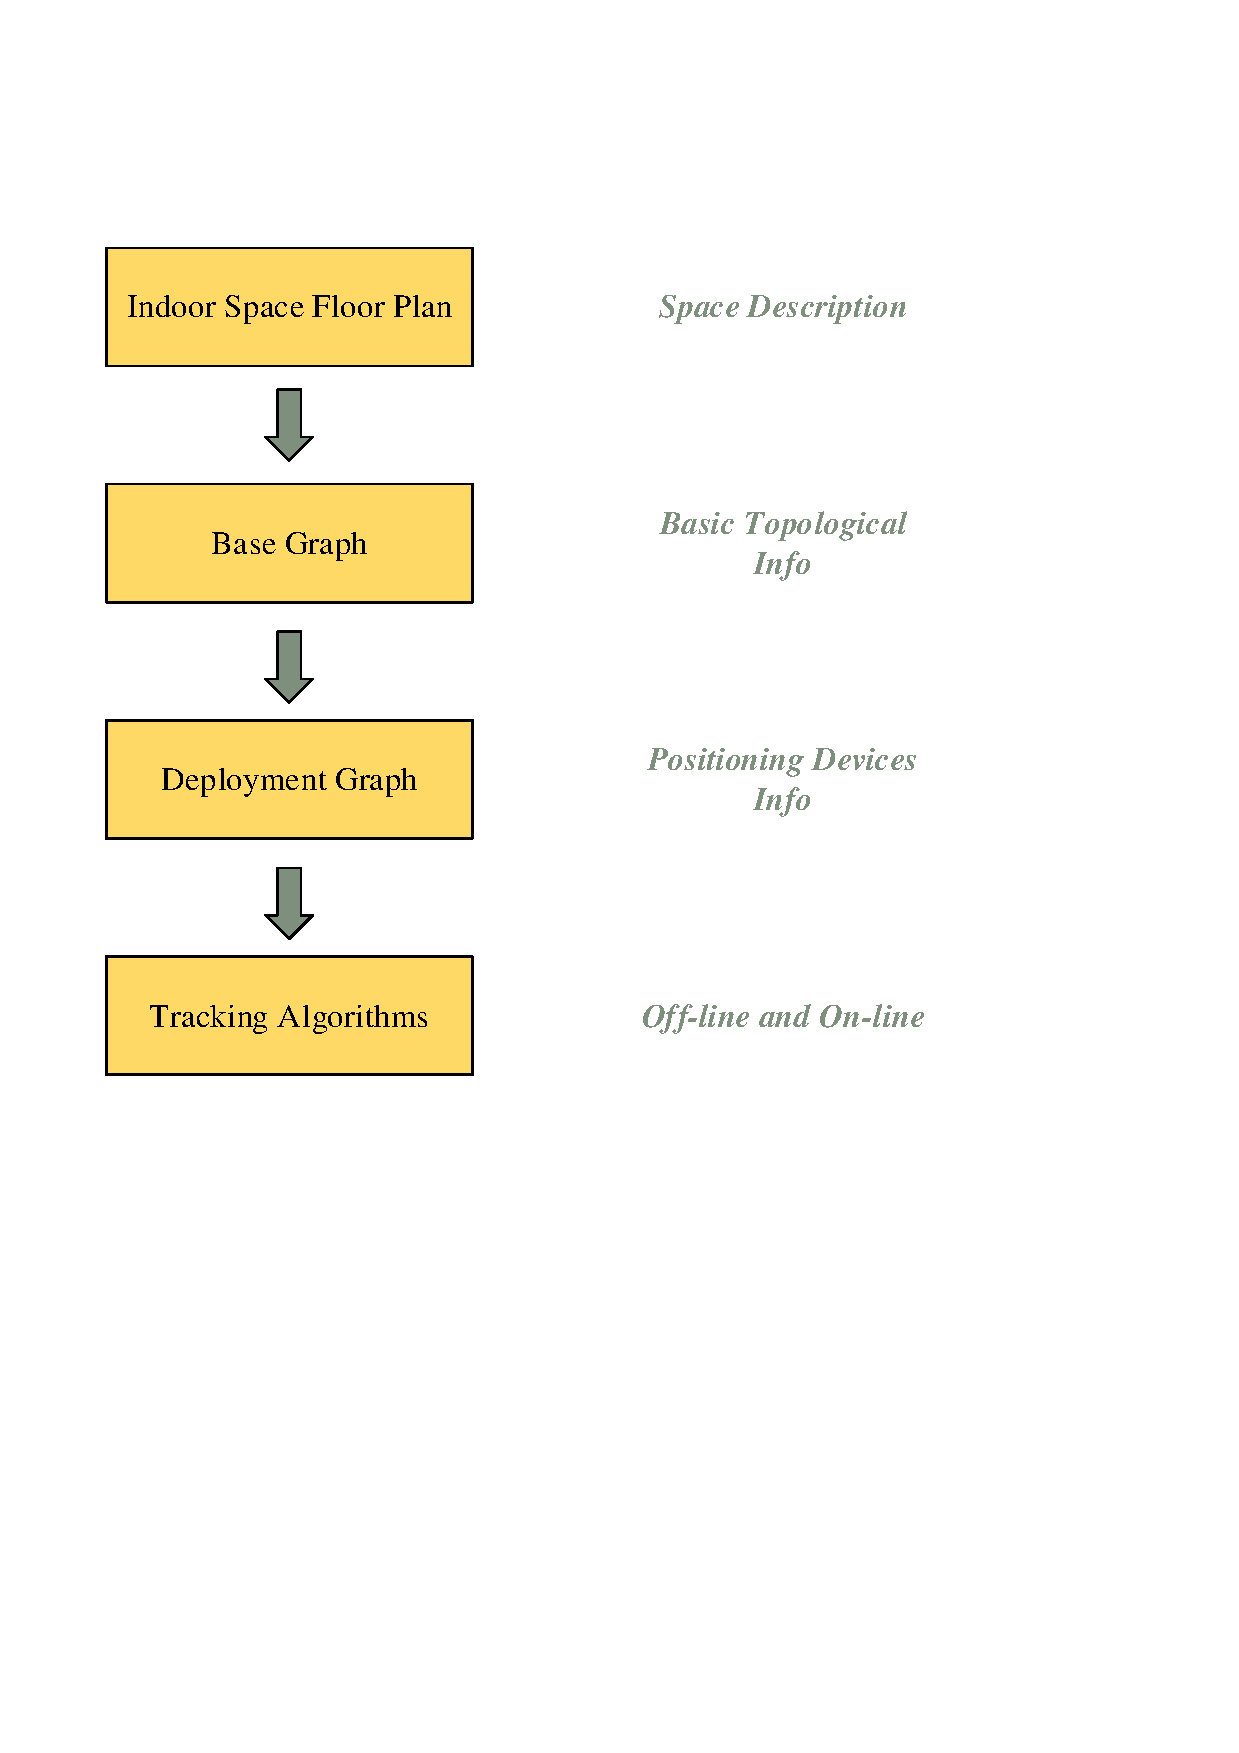
\includegraphics[width=\columnwidth]{figures/2-1/2-1-1.pdf}
    \end{figure}

  \column{.4\textwidth}
    \pause
    \conceptbf{Goal:} \textrm{Improve indoor tracking accuracy from a data management perspective, to capture where a particular object can be at a particular time.}

\end{columns}

\end{frame}

%------------------------------------------------

\begin{frame}
\frametitle{Base Graph Model}

\small{By capturing the essential connectivity and accessibility, \conceptbf{Base Graph} describes the topology of a floor plan of a possibly complex indoor space.}

\begin{columns}[c]

  \column{.45\textwidth}
    \begin{figure}[tb]
      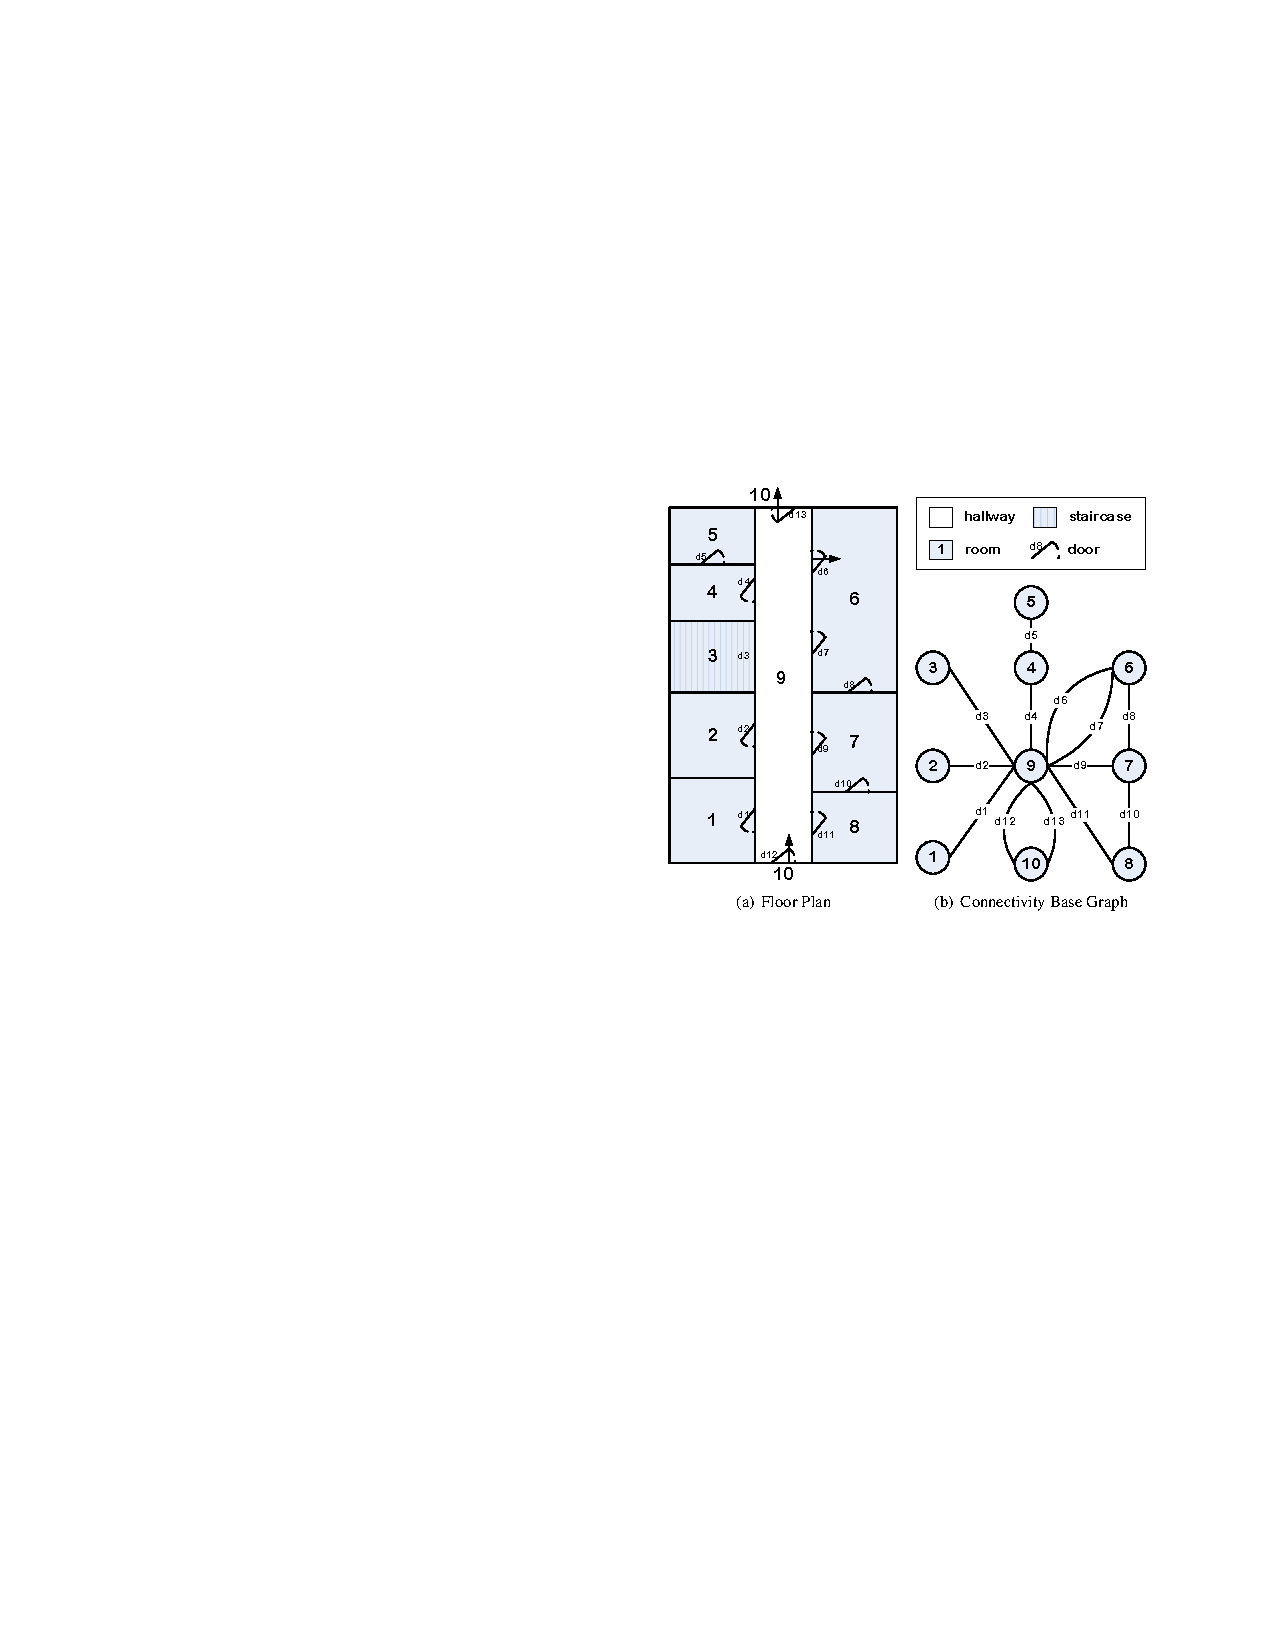
\includegraphics[width=\columnwidth]{figures/2-1/2-1-2.pdf}
    \end{figure}

  \column{.55\textwidth}
    \begin{block}{Connectivity Base Graph}
    a labeled, undirected graph.
      \textrm{
      \begin{itemize}
        \item $\mn{G_{conn} = \{V, E_d, \Sigma_{door}\}}$
        \item $\mn{V}$: each separate partition is represented as a vertex
        \item $\mn{E_d}$: each door is captured as an edge%, i.e., $\mn{(\{v_i,v_j}, k)}$
        \item $\mn{\Sigma_{door}}$: a set of edge labels that represent connections
      \end{itemize}
      }
    \end{block}

\end{columns}
\end{frame}

%------------------------------------------------

\begin{frame}
\frametitle{Base Graph Model}

  \small{\conceptbf{Accessibility Graph} is constructed to represent the movement permitted by doors or connections.}

\begin{columns}[c]

  \column{.45\textwidth}
    \begin{figure}[tb]
      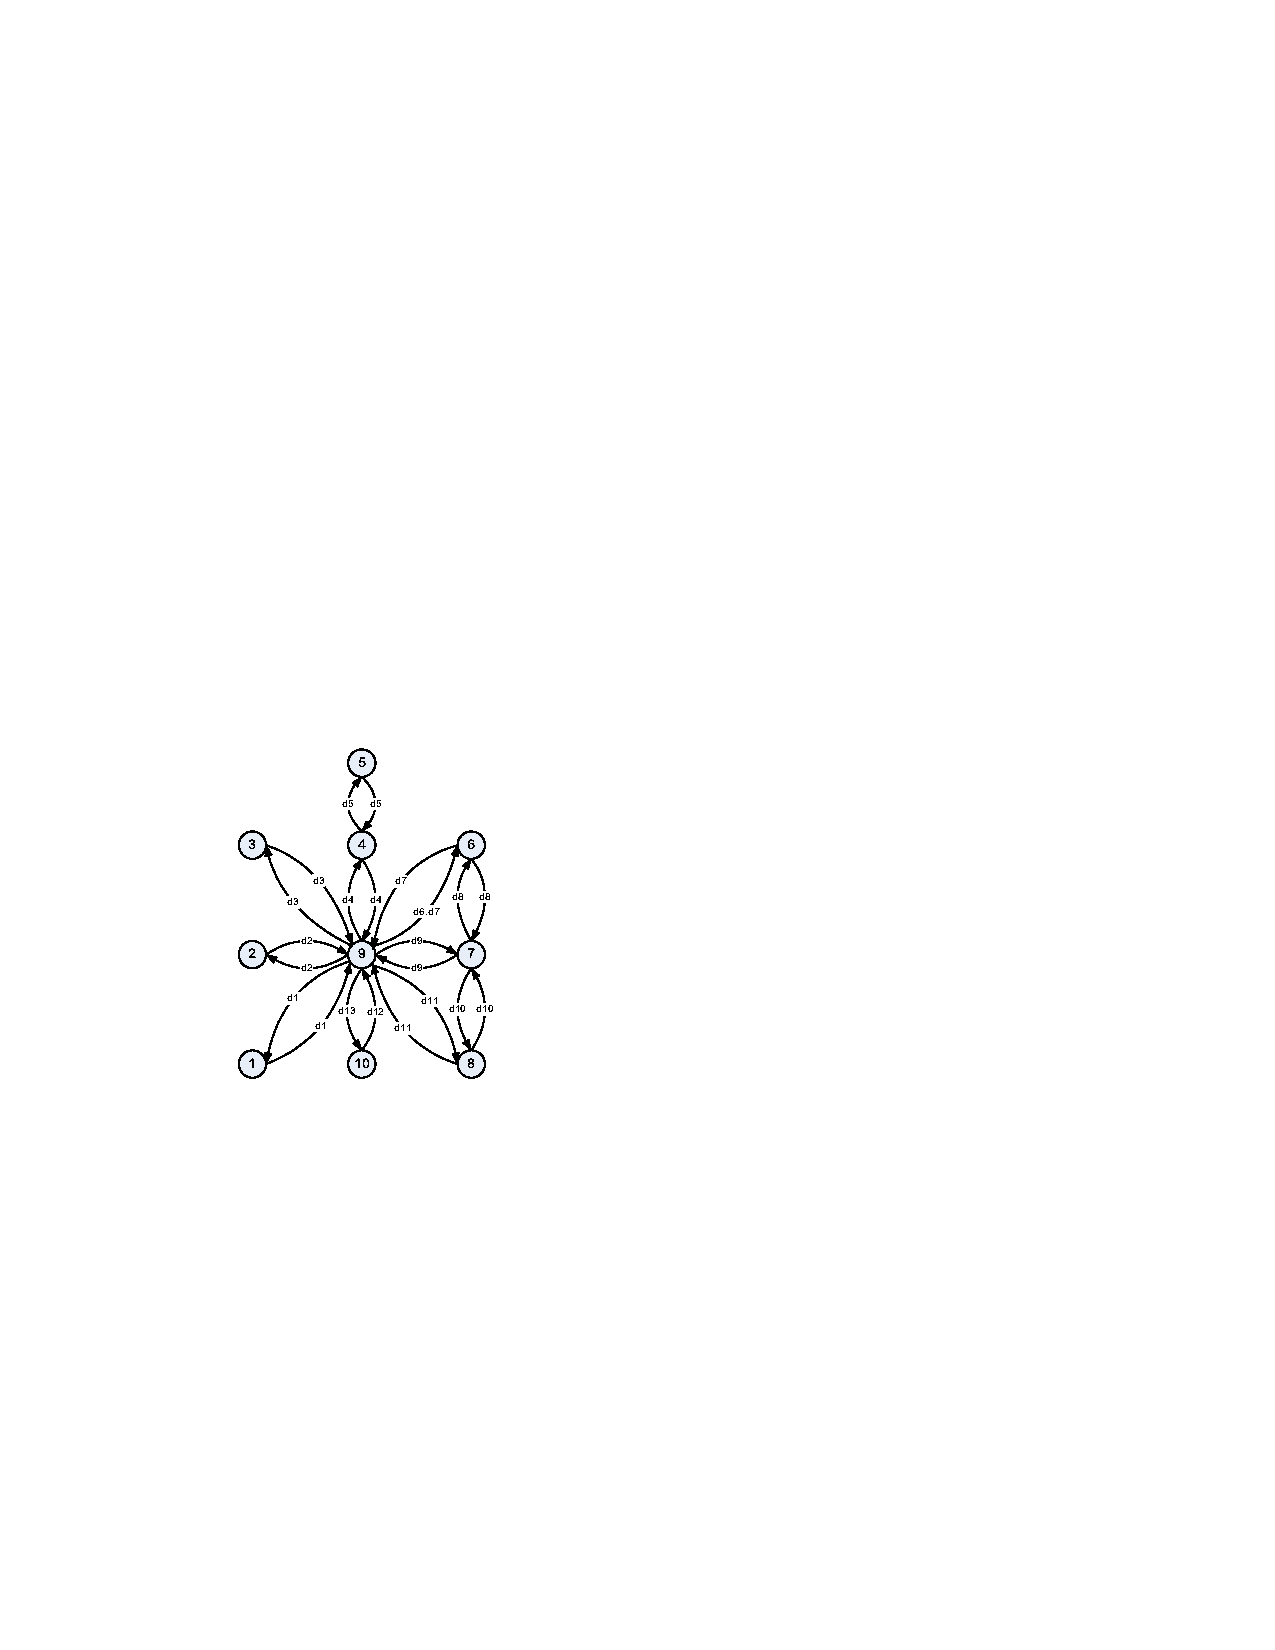
\includegraphics[width=\columnwidth]{figures/2-1/2-1-3.pdf}
    \end{figure}

  \column{.55\textwidth}
    \begin{block}{Accessibility Graph}
    a labeled, directed graph.
      \textrm{
      \begin{itemize}
        \item $\mn{G_{accs} = \{V, E, \Sigma_{door}, l_e\}}$
        \item $\mn{V}$: the set of vertices
        \item $\mn{E}$: the set of directed edges, i.e., $\mn{E=\{\langle v_i, v_j\rangle | v_i, v_j \in V \wedge v_i \neq v_j\}}$
        \item $\mn{l_e}$: a function that maps edges to subsets of the set of doors, i.e., $\mn{l_e : E \rightarrow 2^{\Sigma_{door}}}$
      \end{itemize}
      }
    \end{block}

\end{columns}
\end{frame}

%------------------------------------------------

\begin{frame}
\frametitle{Base Graph Model}

  \small{In addition to the topological information of a floor plan, its geometrical information should also be captured.}
  \\~\\
  \pause

  The \textrm{\em Building Partitions Mapping} is defined as:
  \pause
  \begin{equation}
  \mn{BuildingPartitions: V \rightarrow Ploygons}
  \end{equation}
  \\~\\
  \pause

  The \textrm{\em Doors Mapping} is defined as:
  \pause
  \begin{equation}
  \mn{Doors: \Sigma_{door} \rightarrow Line~Segments}
  \end{equation}

\end{frame}

%------------------------------------------------


\begin{frame}
\frametitle{RFID Deployment Graph Model}

\begin{itemize}
  \item RFID based proximity analysis
      \begin{itemize}
        %\item a record is produced when a \emph{RFID tag} approaches a \emph{RFID reader}.
        \item RFID readers deployment may cover only part of the space, or it may be capable of only detecting some movements in the space.
        \item assume that all RFID readers have disjoint activation ranges.
      \end{itemize}
  \item Types of RFID readers
      \begin{itemize}
        \item \conceptbf{Partitioning Readers} partition the indoor space into cells in the sense that an object cannot move from one cell to another without being observed.
        \item \conceptbf{Presence Readers} simply observe the presence(and non-presence) of tags in their activation ranges.
      \end{itemize}
\end{itemize}

\end{frame}

%------------------------------------------------

\begin{frame}
\frametitle{RFID Deployment Graph Model}

\small{Vertices represent cells. A directed edge indicates that one can move from one cell to another without entering other cells, which is detected by a corresponding partitioning reader.}

\begin{columns}[c]

  \column{.45\textwidth}
    \begin{figure}[tb]
      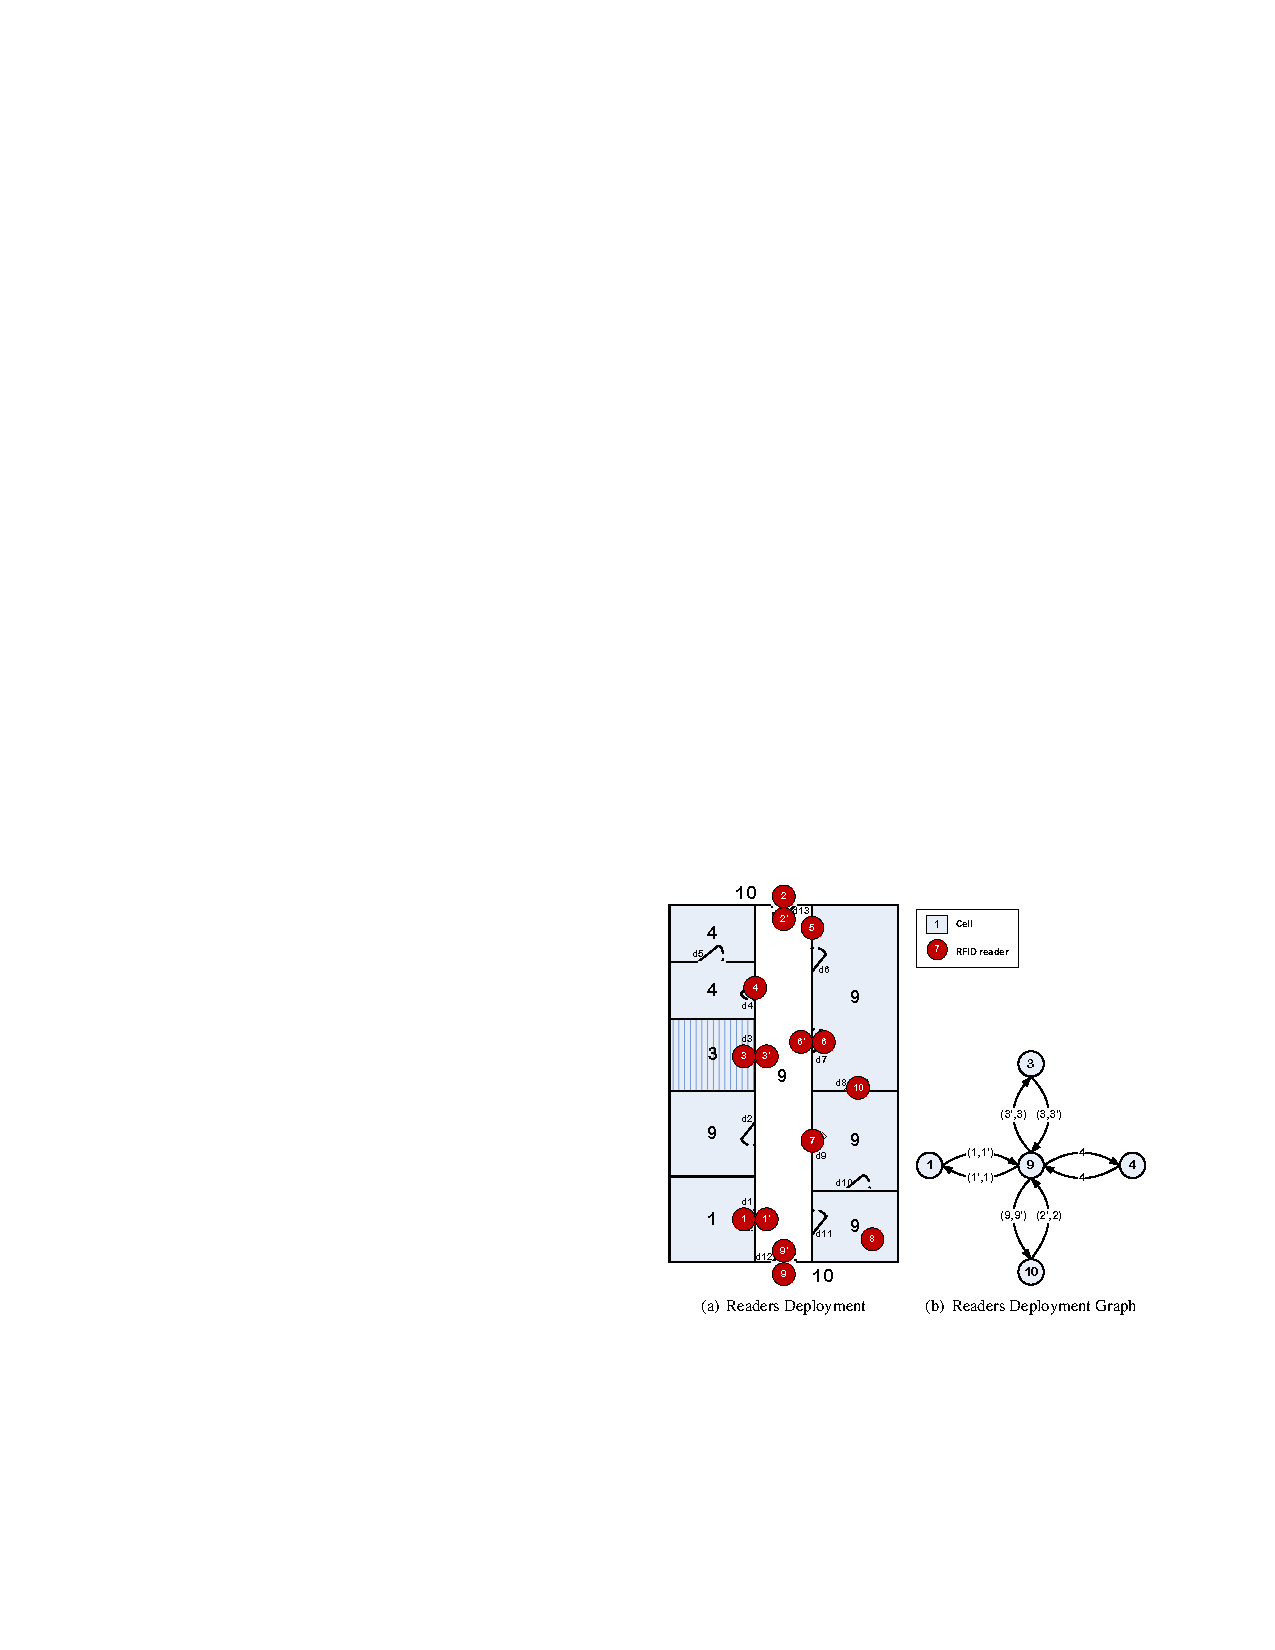
\includegraphics[width=\columnwidth]{figures/2-1/2-1-4.pdf}
    \end{figure}

  \column{.55\textwidth}
    \begin{block}{RFID Deployment Graph}
    a labeled, directed graph.
      \textrm{
      \begin{itemize}
        \item $\mn{G_{RFID} = \{C, E_r, \Sigma_{reader}, l_e\}}$
        \item $\mn{C}$: the set of the vertices
        \item $\mn{E_r}$: An edge is an ordered pair $\mn{\langle c_i, c_j \rangle}$ of distinct vertices from $\mn{C}$
        \item $\mn{l_e}$ maps an edge to a partitioning reader (pair), i.e., $\mn{E_r \rightarrow 2^{\Sigma_{reader}} \cup 2^{\Sigma_{reader} \times \Sigma_{reader}}}$
      \end{itemize}
      }
    \end{block}

\end{columns}
\end{frame}

%------------------------------------------------

\begin{frame}
\frametitle{RFID Deployment Graph Construction}

  \small{Each cell created by partitioning readers corresponds to one or more base graph partitions.}
  \pause
  \begin{equation}
  \mn{Cells: V \rightarrow C}
  \end{equation}
  \\~\\
  \pause

  \small{For each RFID reader, record its accurate deployment location and activation range.}
  \pause
  \begin{equation}
  \begin{split}
  \mn{Mapping~1}: & \mn{\Sigma_{reader} \rightarrow \{ (loc, range, flag)~|~loc \in R^2 \wedge} \\
    & \mn{range \in (0,d_{max}] \wedge flag \in \{ PAR, PRE \} \}}
  \end{split}
  \end{equation}
  \\~\\
  \pause

  \small{A mapping of readers to the cells that their activation ranges intersect is introduced as:}
  \pause
  \begin{equation}
  \mn{
  Mapping~2: \Sigma_{reader} \rightarrow 2^C
  }
  \end{equation}

\end{frame}

%------------------------------------------------

\begin{frame}
\frametitle{RFID Deployment Graph Construction}

\begin{columns}[c]

  \column{.47\textwidth}
    \begin{figure}[tb]
      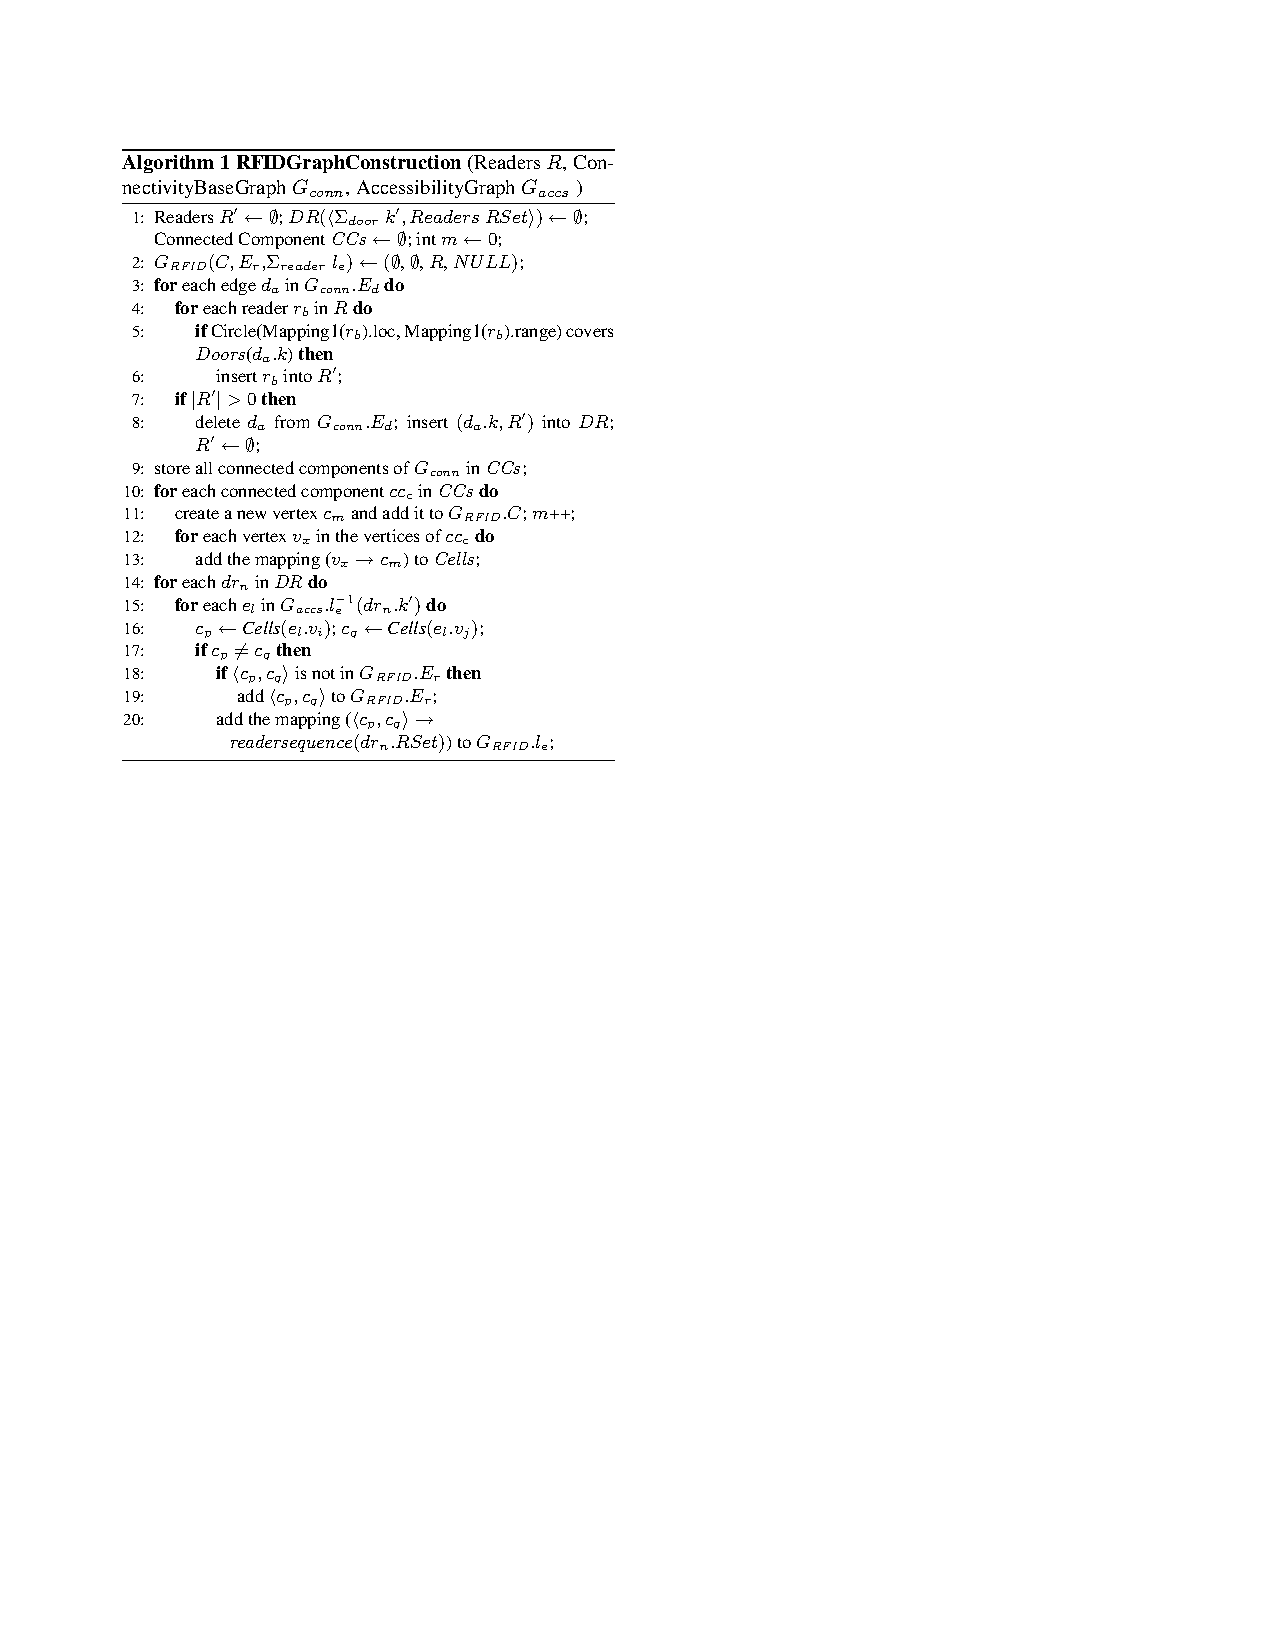
\includegraphics[width=\columnwidth]{figures/2-1/2-1-5.pdf}
    \end{figure}

  \column{.53\textwidth}
  \ssize{
    \begin{enumerate}
      \pause
      \item Input: \textrm{the reader set $\mn{R}$, the connectivity base graph $\mn{G_{conn}}$, the accessibility graph $\mn{G_{accs}}$} \pause
      \item Lines 1--2: \textrm{Initialize $\mn{G_{RFID}}$, $\mn{DR}$, $\mn{CCs}$} \pause
      \item Lines 3--8: \textrm{the relationship of which door is covered by which readers is captured in $\mn{DR}$} \pause
      \item Lines 9--13: \textrm{a deployment graph vertex is created for each $\mn{CC}$, mapping $\mn{Cells}$ is also stored} \pause
      \item Lines 14--20: \textrm{for each door in $\mn{DR}$, determine if its edges' head and tail are mapped to different cells. If so, add an edge to deployment graph. Function $\mn{readersequence}$ returns the possible reader sequence for that edge}
    \end{enumerate}
  }
  \end{columns}

\end{frame}

%------------------------------------------------

\begin{frame}
\frametitle{RFID-based Indoor Tracking}

  \small{\conceptbf{Raw Trajectories}: \textrm{Sequences of RFID Tag Observation}}

  \begin{columns}[c]

  \column{.47\textwidth}
    \begin{figure}[tb]
      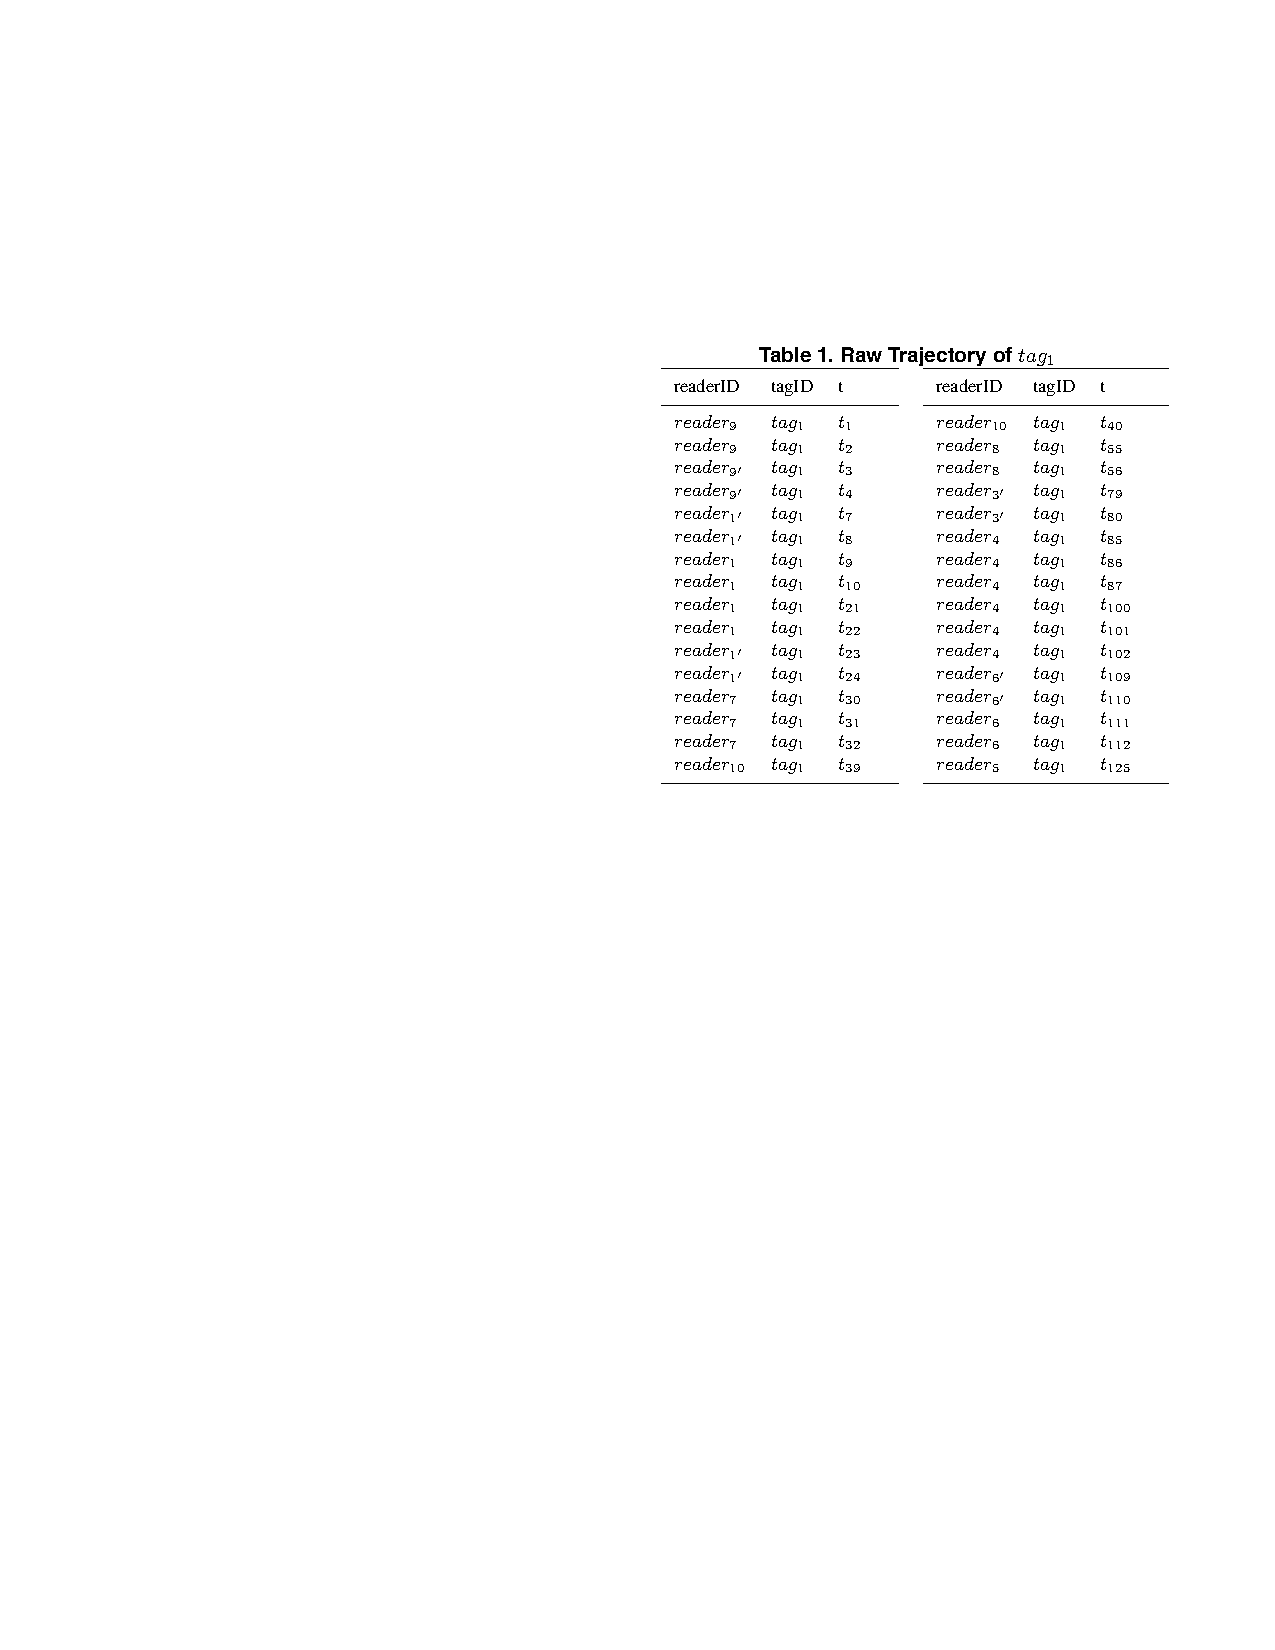
\includegraphics[width=\columnwidth]{figures/2-1/2-1-6.pdf}
    \end{figure}
    \ssize{\textit{
      1. each reader detects and reports tags with a sampling rate \\
      2. formatted as $\mn{\langle readerID, tagID, t \rangle}$
    }}

  \column{.53\textwidth}
    \begin{figure}[tb]
      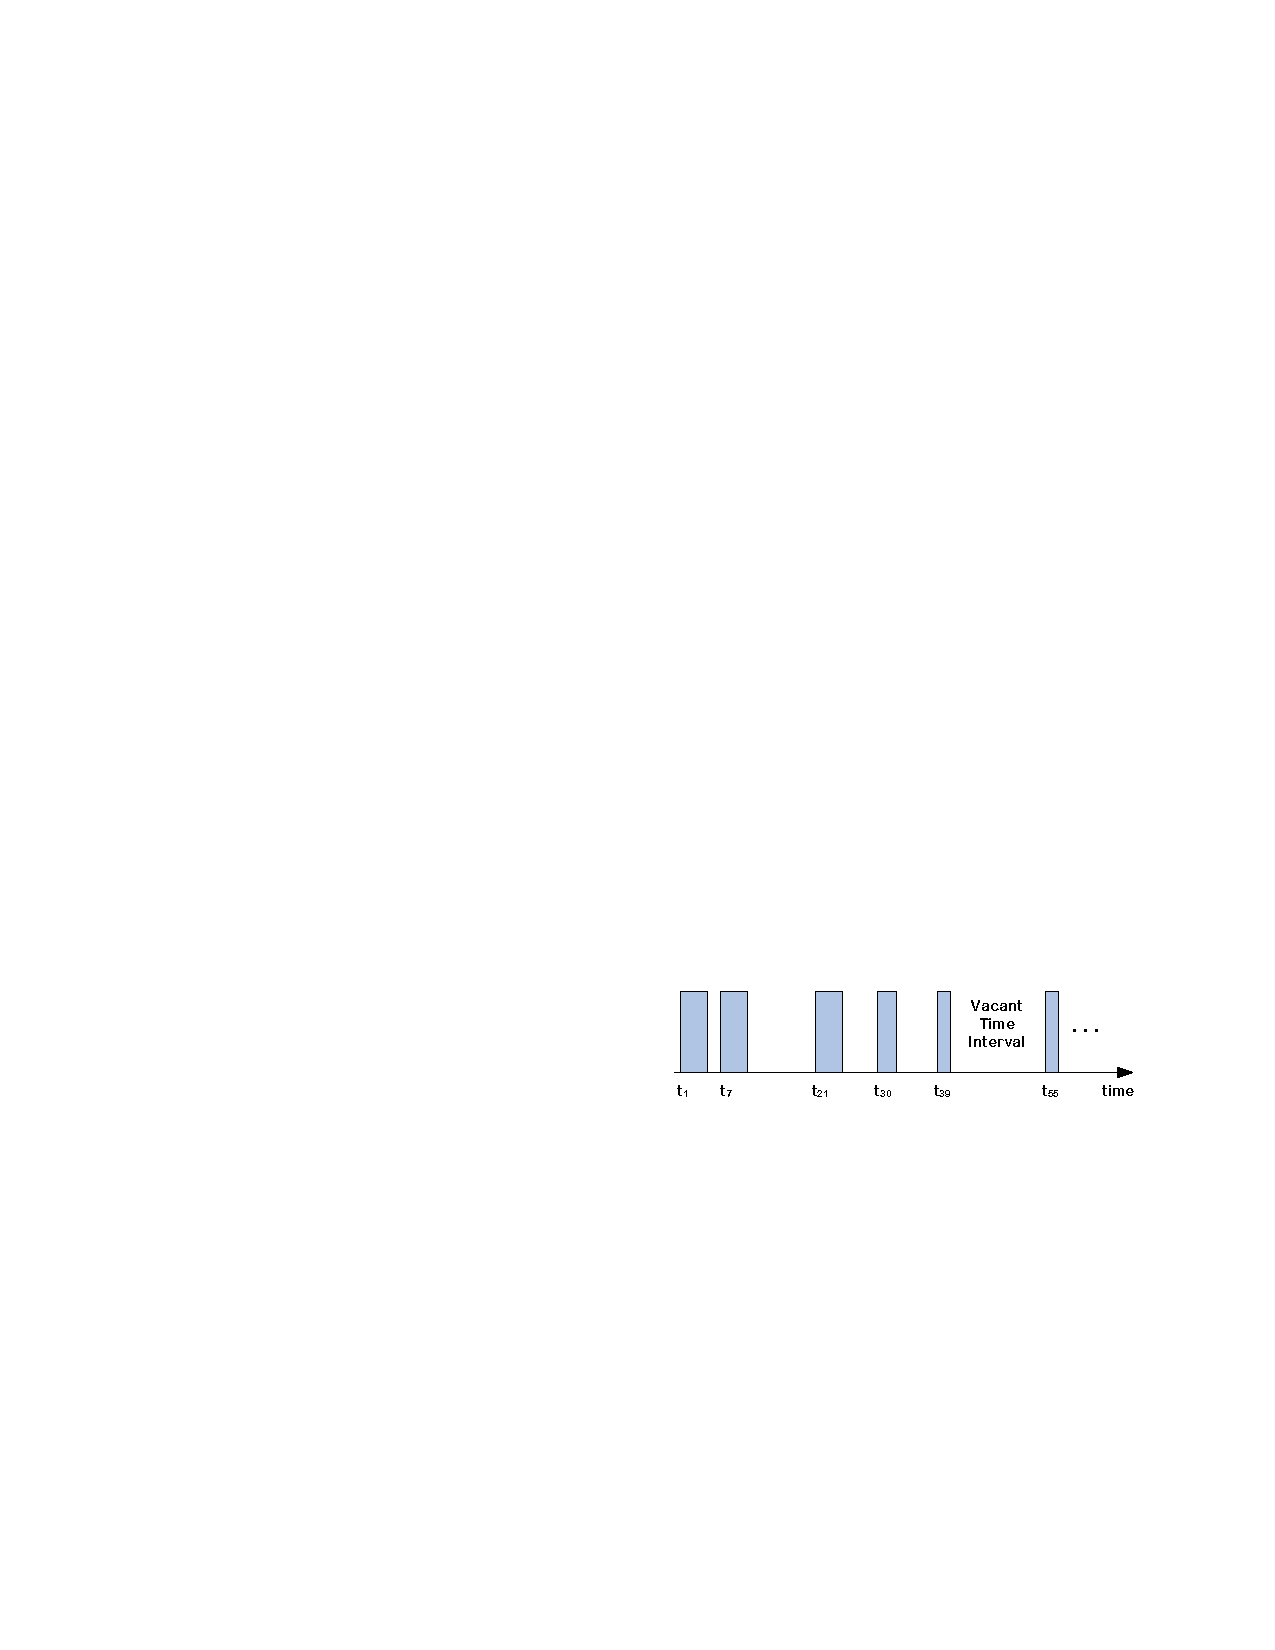
\includegraphics[width=\columnwidth]{figures/2-1/2-1-7.pdf}
    \end{figure}

    \vspace{-15pt}
    \ssize{
      \begin{itemize}
        \pause
        \item \emph{vacant time intervals}: unable to observe the moving objects \pause
        \item to search RFID deployment graph to infer the possible regions of moving object \pause
        \item to apply maximum speed position interpolation to further shrink the possible regions~\cite{civilis2005techniques, pfoser1999capturing}
      \end{itemize}
    }

  \end{columns}

\end{frame}

%------------------------------------------------

\begin{frame}
\frametitle{RFID Readings Pre-processing}

  \small{Step-1's output is used in on-line tracking, while Step-2's is used in off-line tracking}

  \begin{columns}[c]

  \column{.47\textwidth}
    \begin{figure}[tb]
      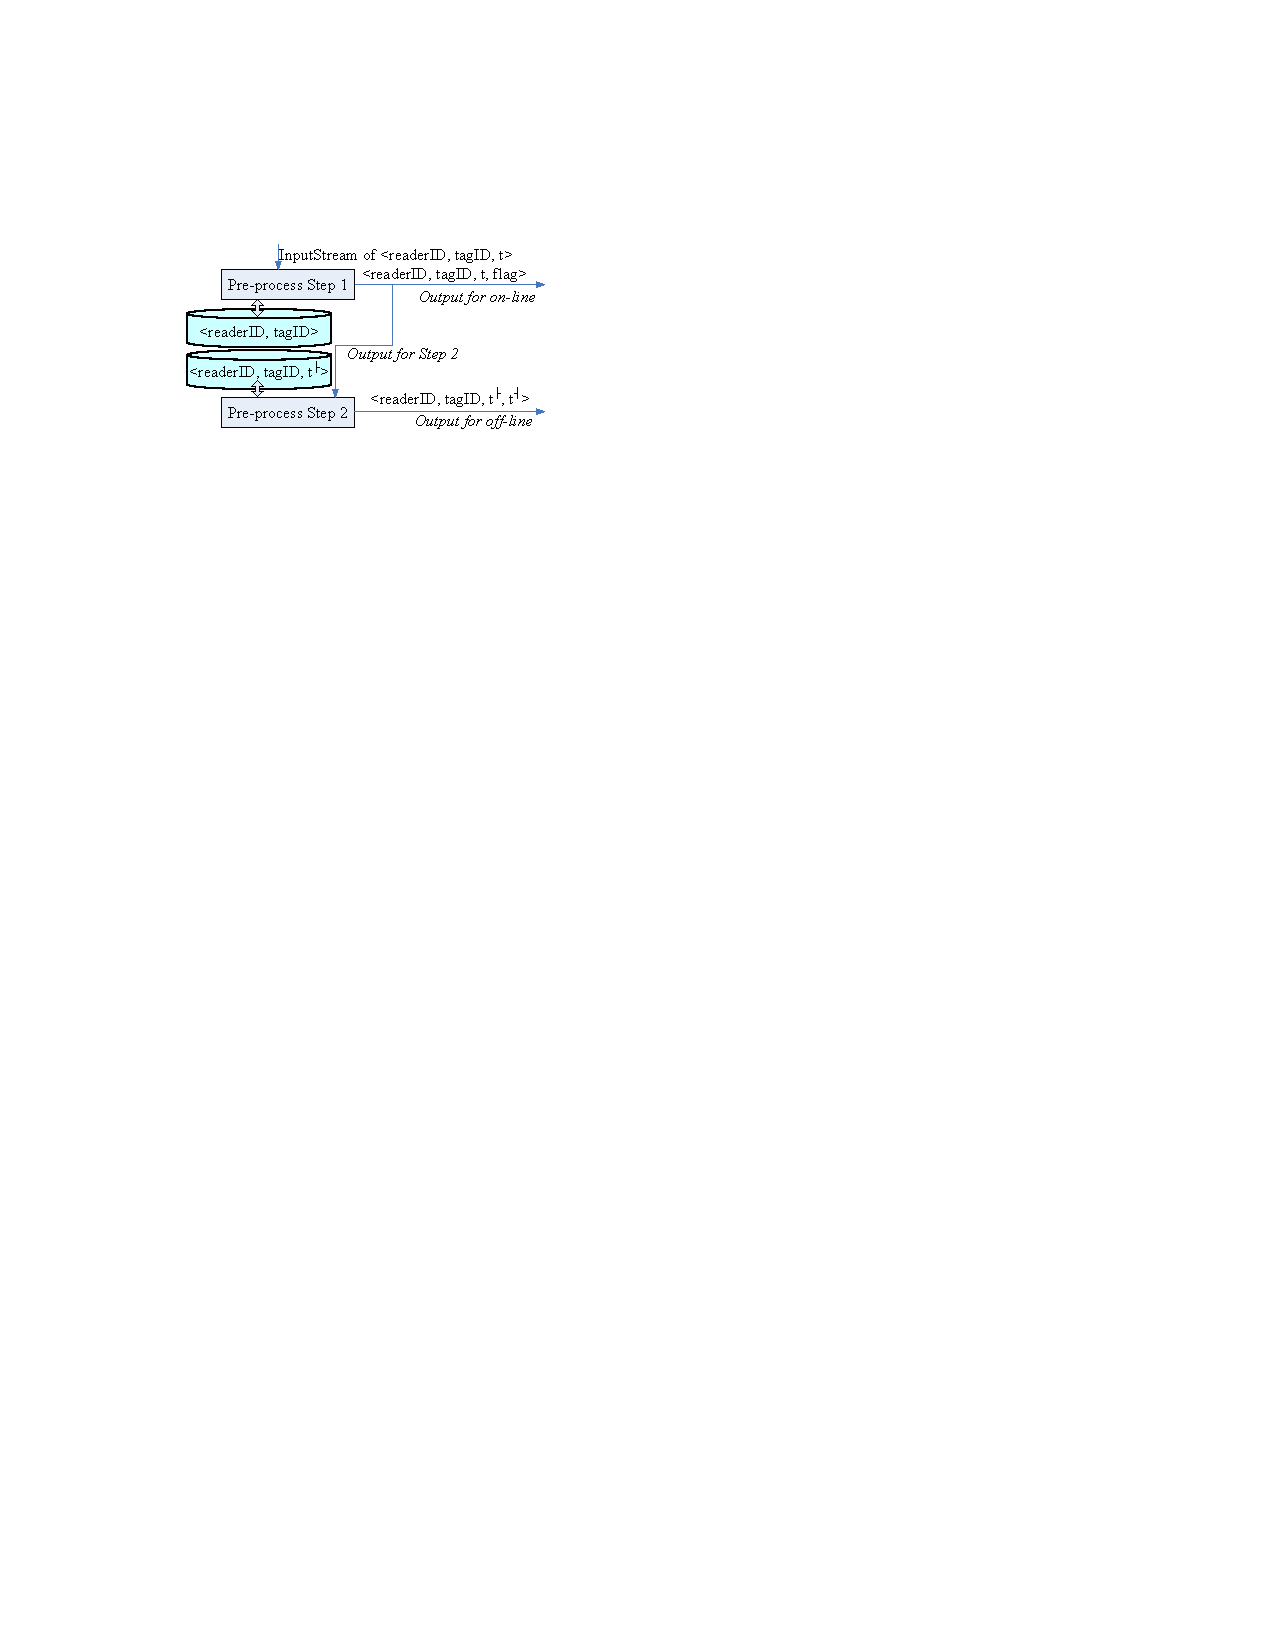
\includegraphics[width=\columnwidth]{figures/2-1/2-1-8.pdf}
    \end{figure}

  \column{.53\textwidth}
    \begin{itemize}
        \item $\mn{Flag \in \{ START, END \}}$
        \item $\mn{START} \rightarrow$ \textrm{enters the range}
        \item $\mn{END} \rightarrow$ \textrm{leaves the range}
    \end{itemize}

  \end{columns}

\end{frame}

%------------------------------------------------

\begin{frame}
\frametitle{Off-line Tracking (Refinement Step 1)}

  \begin{columns}[c]

  \column{.43\textwidth}
    \vspace{-15pt}
    \begin{figure}[tb]
      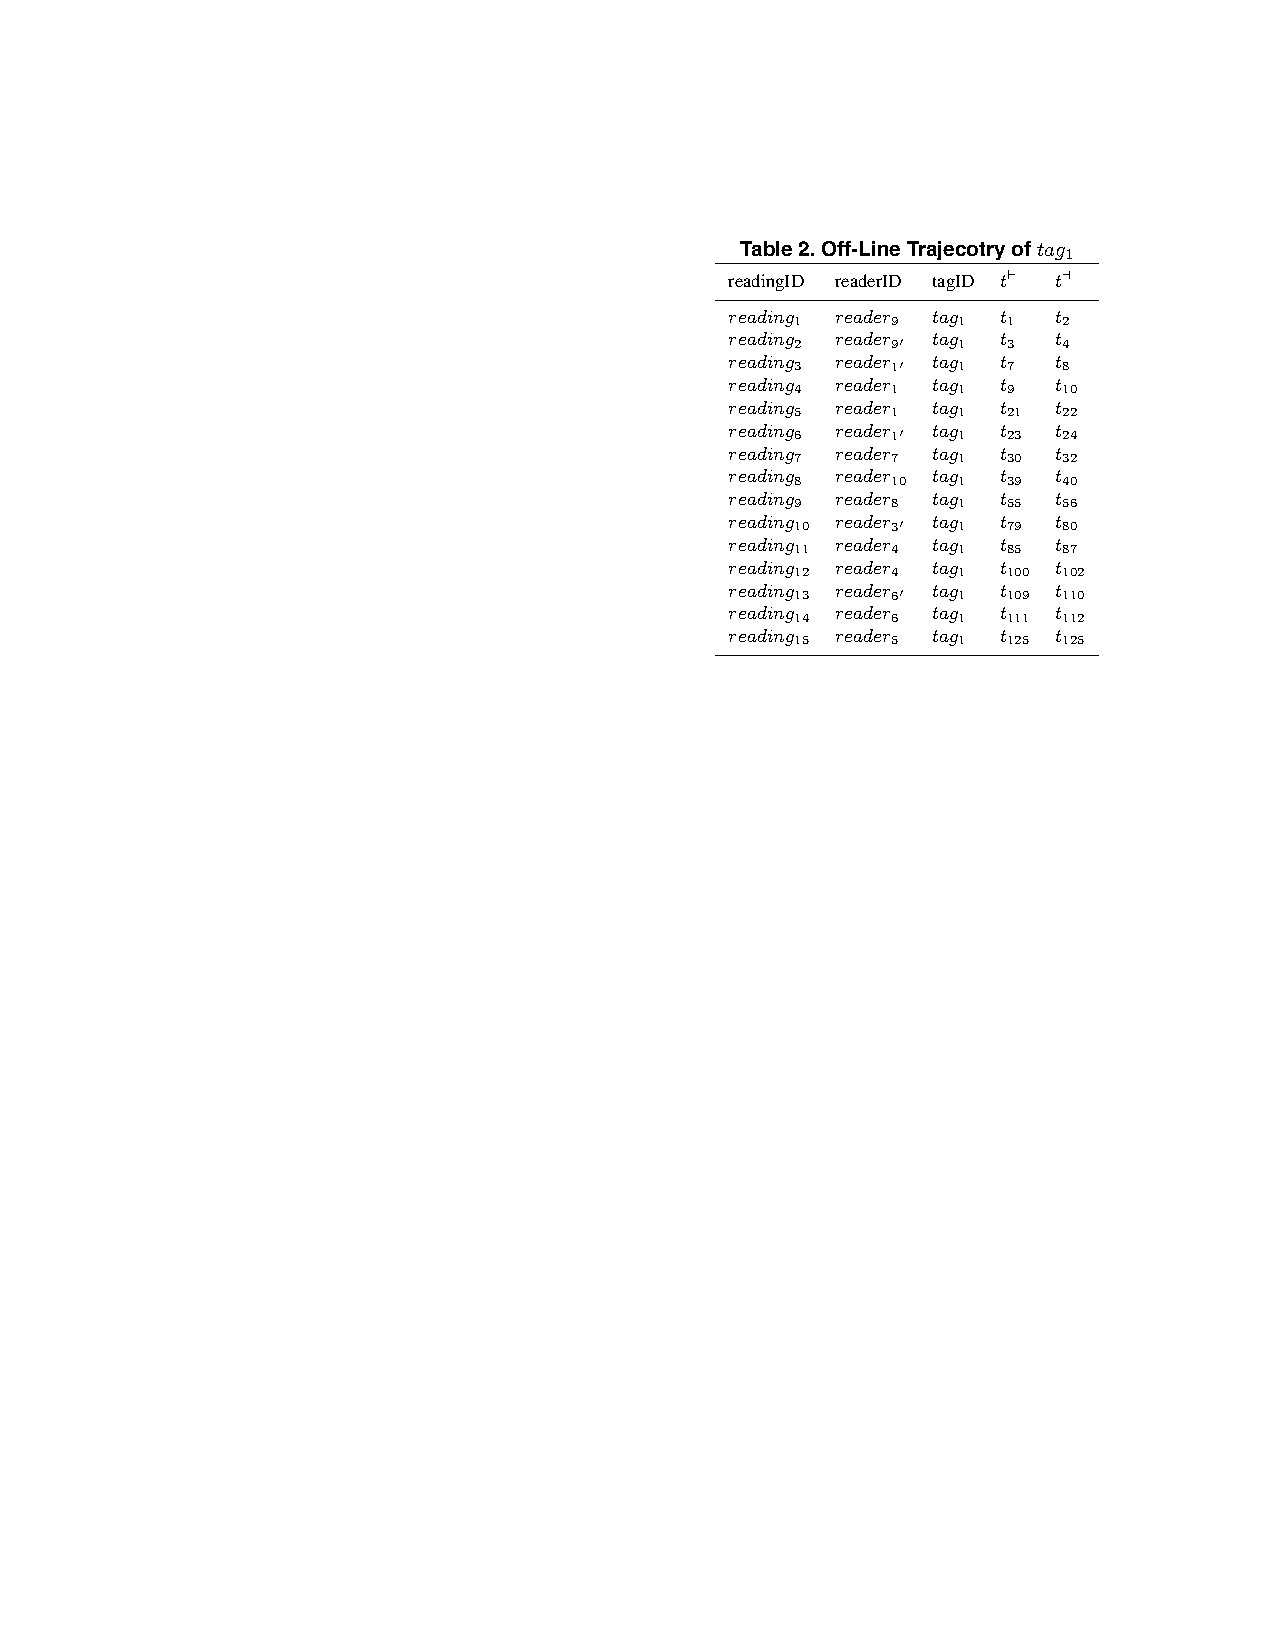
\includegraphics[width=0.92\columnwidth]{figures/2-1/2-1-9.pdf}
    \end{figure}
    \vspace{-20pt}
    \begin{figure}[tb]
      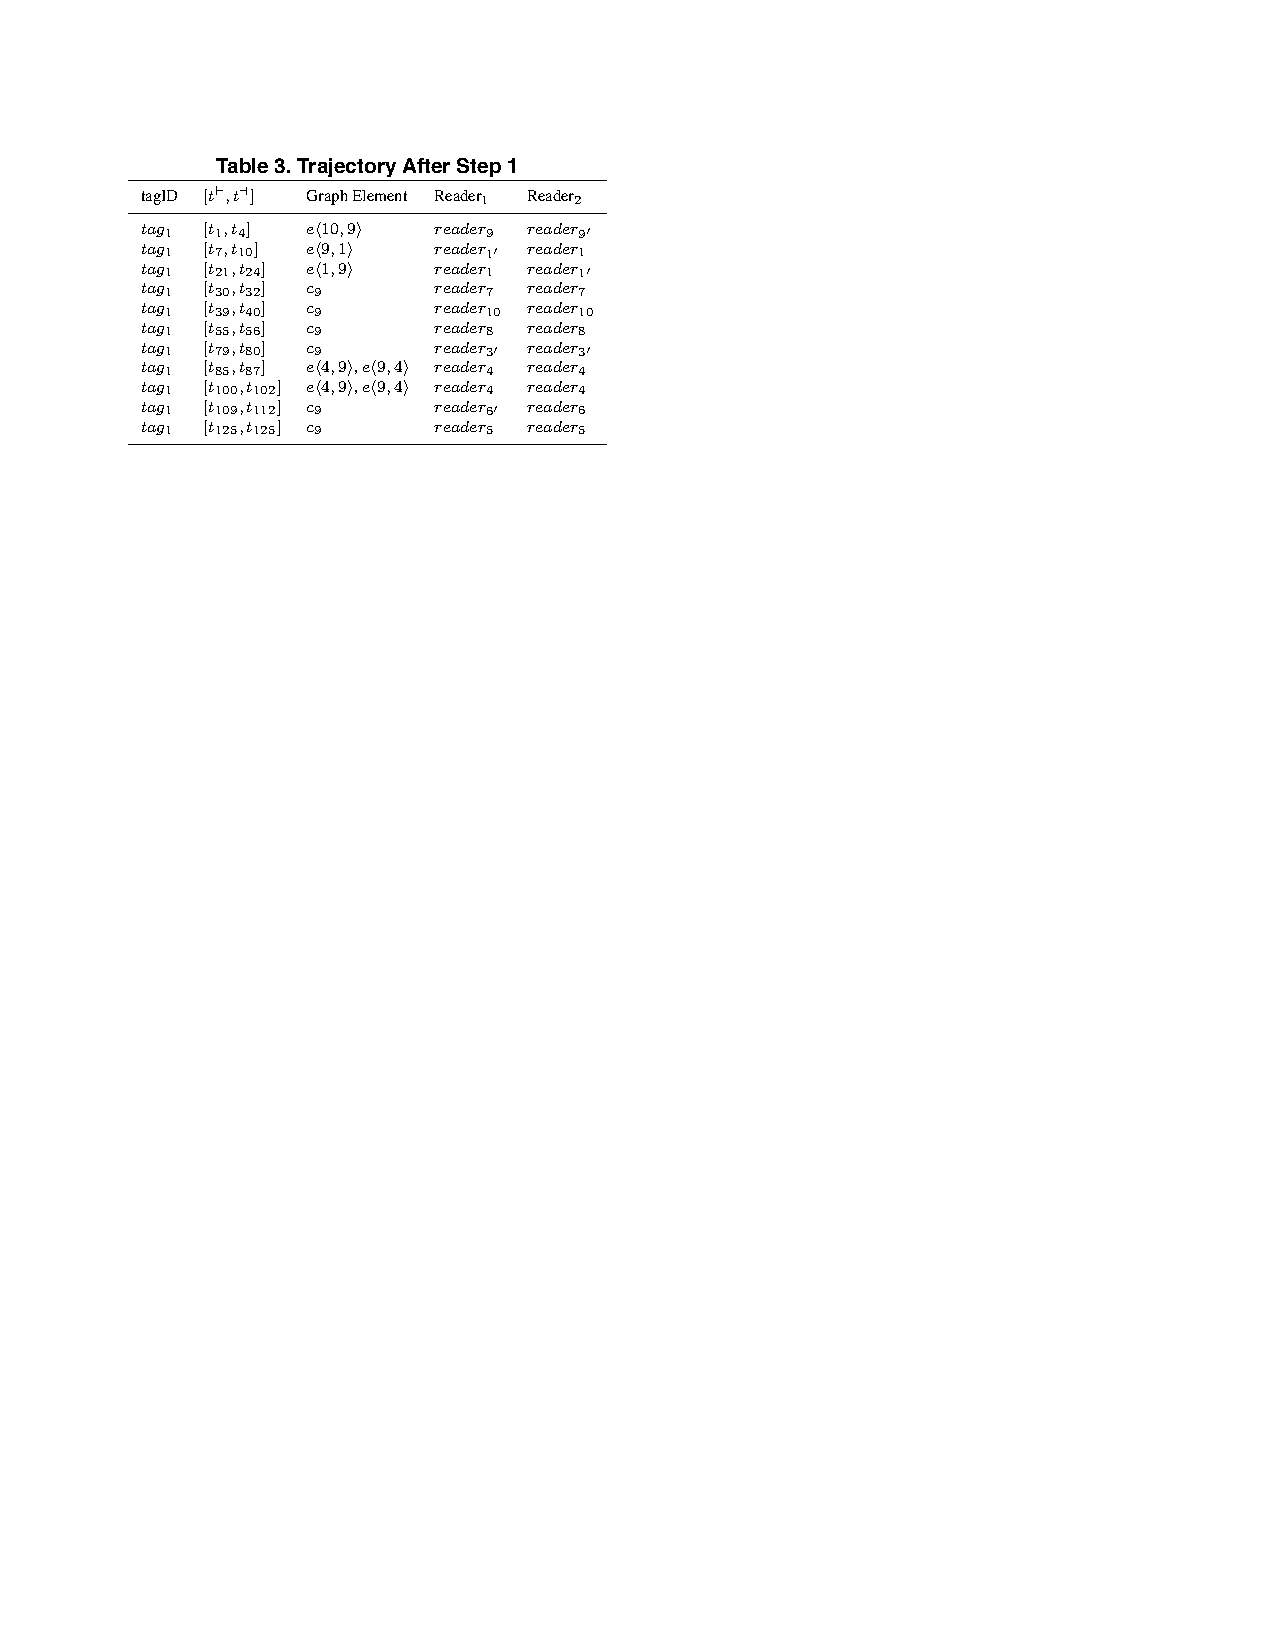
\includegraphics[width=\columnwidth]{figures/2-1/2-1-10.pdf}
    \end{figure}


  \column{.57\textwidth}
  \fsize{
    \begin{itemize}
      \item Step 1 transforms an RFID reading sequence to corresponding vertices or edges in deployment graph
      \item If two consecutive reading sequences are \emph{contiguous}, they should stem from a partitioning pair, which map to an edge
      \item Otherwise, should come from either a single $\mn{PRE}$ or a $\mn{PAR}$ reader
      \item A $\mn{PAR}$ is replaced by the set of corresponding edges according to $\mn{G_{RFID}.{l_e}^{-1}}$
      \item A $\mn{PRE}$ always corresponds to one or several cells according to $\mn{Mapping~2}$
    \end{itemize}
  }
  \end{columns}

\end{frame}

%------------------------------------------------

\begin{frame}
\frametitle{Off-line Tracking (Refinement Step 2)}

\begin{columns}[c]

  \column{.43\textwidth}
  \vspace{-15pt}
  \begin{figure}[tb]
    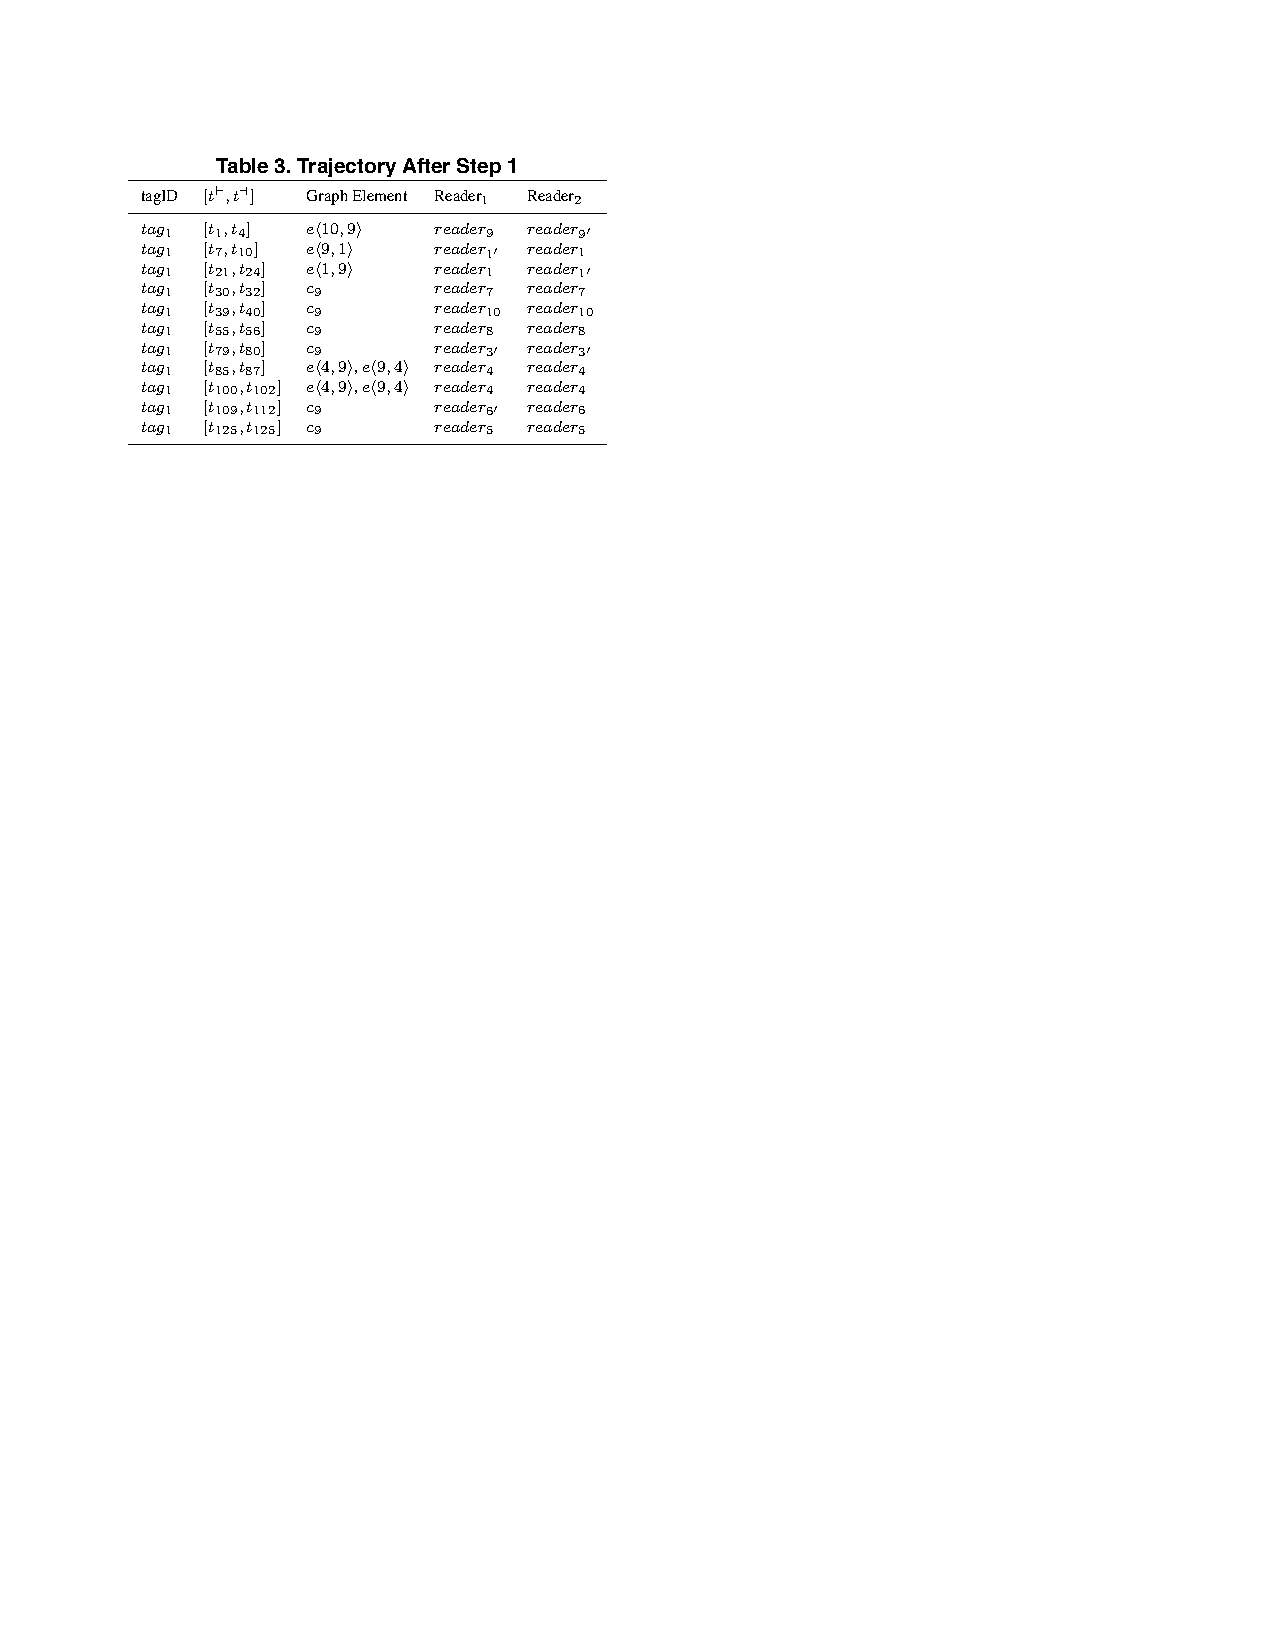
\includegraphics[width=\columnwidth]{figures/2-1/2-1-10.pdf}
  \end{figure}
  \vspace{-20pt}
  \begin{figure}[tb]
    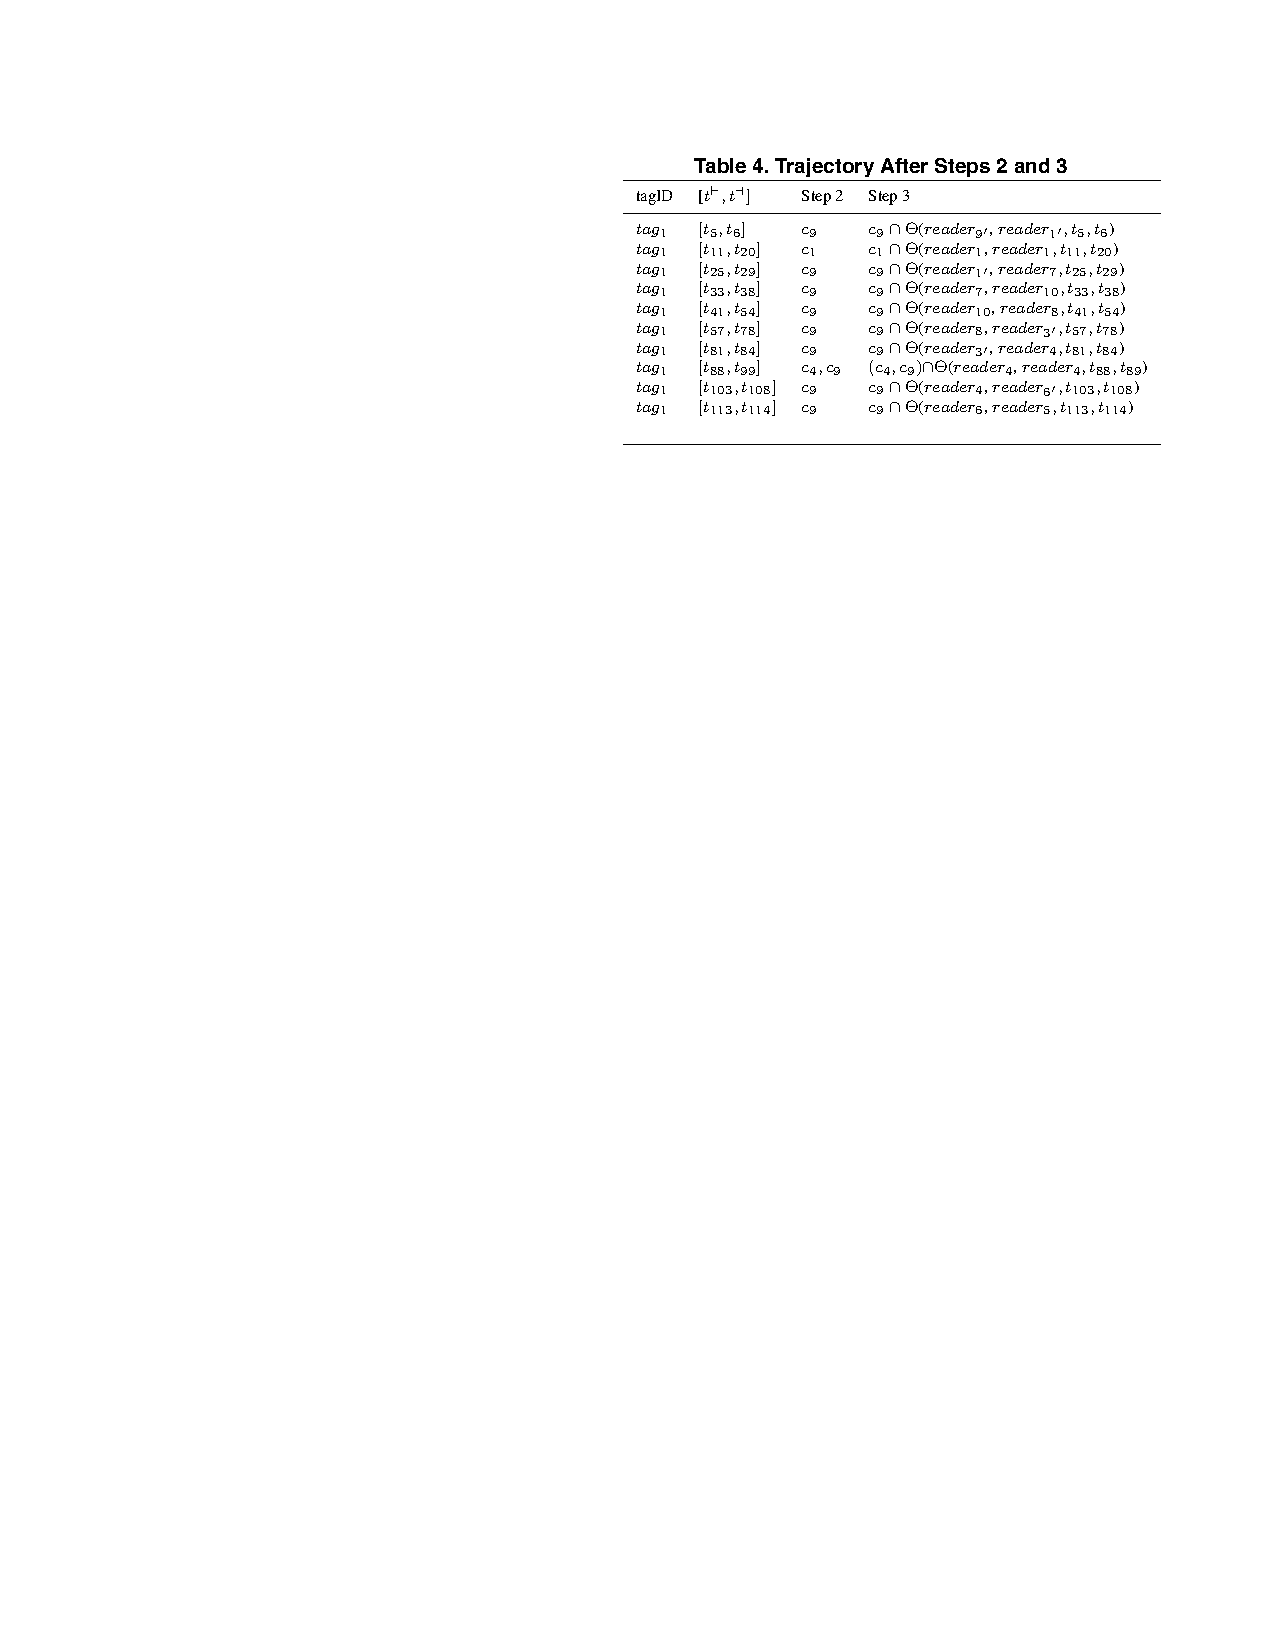
\includegraphics[width=\columnwidth]{figures/2-1/2-1-11.pdf}
  \end{figure}


  \column{.57\textwidth}
  \fsize{
    \begin{itemize}
      \item The \emph{graph elements} from Step 1 indicates some region(s) within which the object may be in during the vacant time interval
      \item Check its previous record's tail element and current record's head element, select their intersection as Step 2's candidate
    \end{itemize}
  }

\end{columns}

\end{frame}

%------------------------------------------------

\begin{frame}
\frametitle{Off-line Tracking (Refinement Step 3)}

\begin{columns}[c]

\column{.48\textwidth}
\begin{itemize}
\ssize{
  \item Calculate the \emph{possible region} $\mn{\Theta}$ according to maximum speed limit

  \item Circle based possible region
    \begin{itemize}
      \tiny{
        \item locations: $\mn{P_{9'}}$, $\mn{P_{1'}}$
        \item activation ranges: $\mn{R_{9'}}$, $\mn{R_{1'}}$
        \item for $\mn{t_x \in [ t_5, t_6 ]}$, $\mn{\Delta t_1 = t_x - reading_2.t^{\vdash}}$, $\mn{\Delta t_2 = reading_3.t^{\dashv} - t_x}$
        \item $\mn{R_3 = R_{9'} + V_{max} * \Delta t_1}$, $\mn{R_5 = R_{1'} + V_{max} * \Delta t_2}$
      }
    \end{itemize}

  \item Ellipse based possible region
  \begin{itemize}
      \tiny{
        \item foci: two points belonging to the circle centered at $\mn{P_{9'}}$, $\mn{P_{1'}}$
        \item length of major axis is:
          \begin{equation*}
            \mn{2a = V_{max} * (\Delta t_1 + \Delta t_2)}
          \end{equation*}
      }
  \end{itemize}
}
\end{itemize}

\column{.52\textwidth}
\vspace{-15pt}
\begin{figure}[tb]
  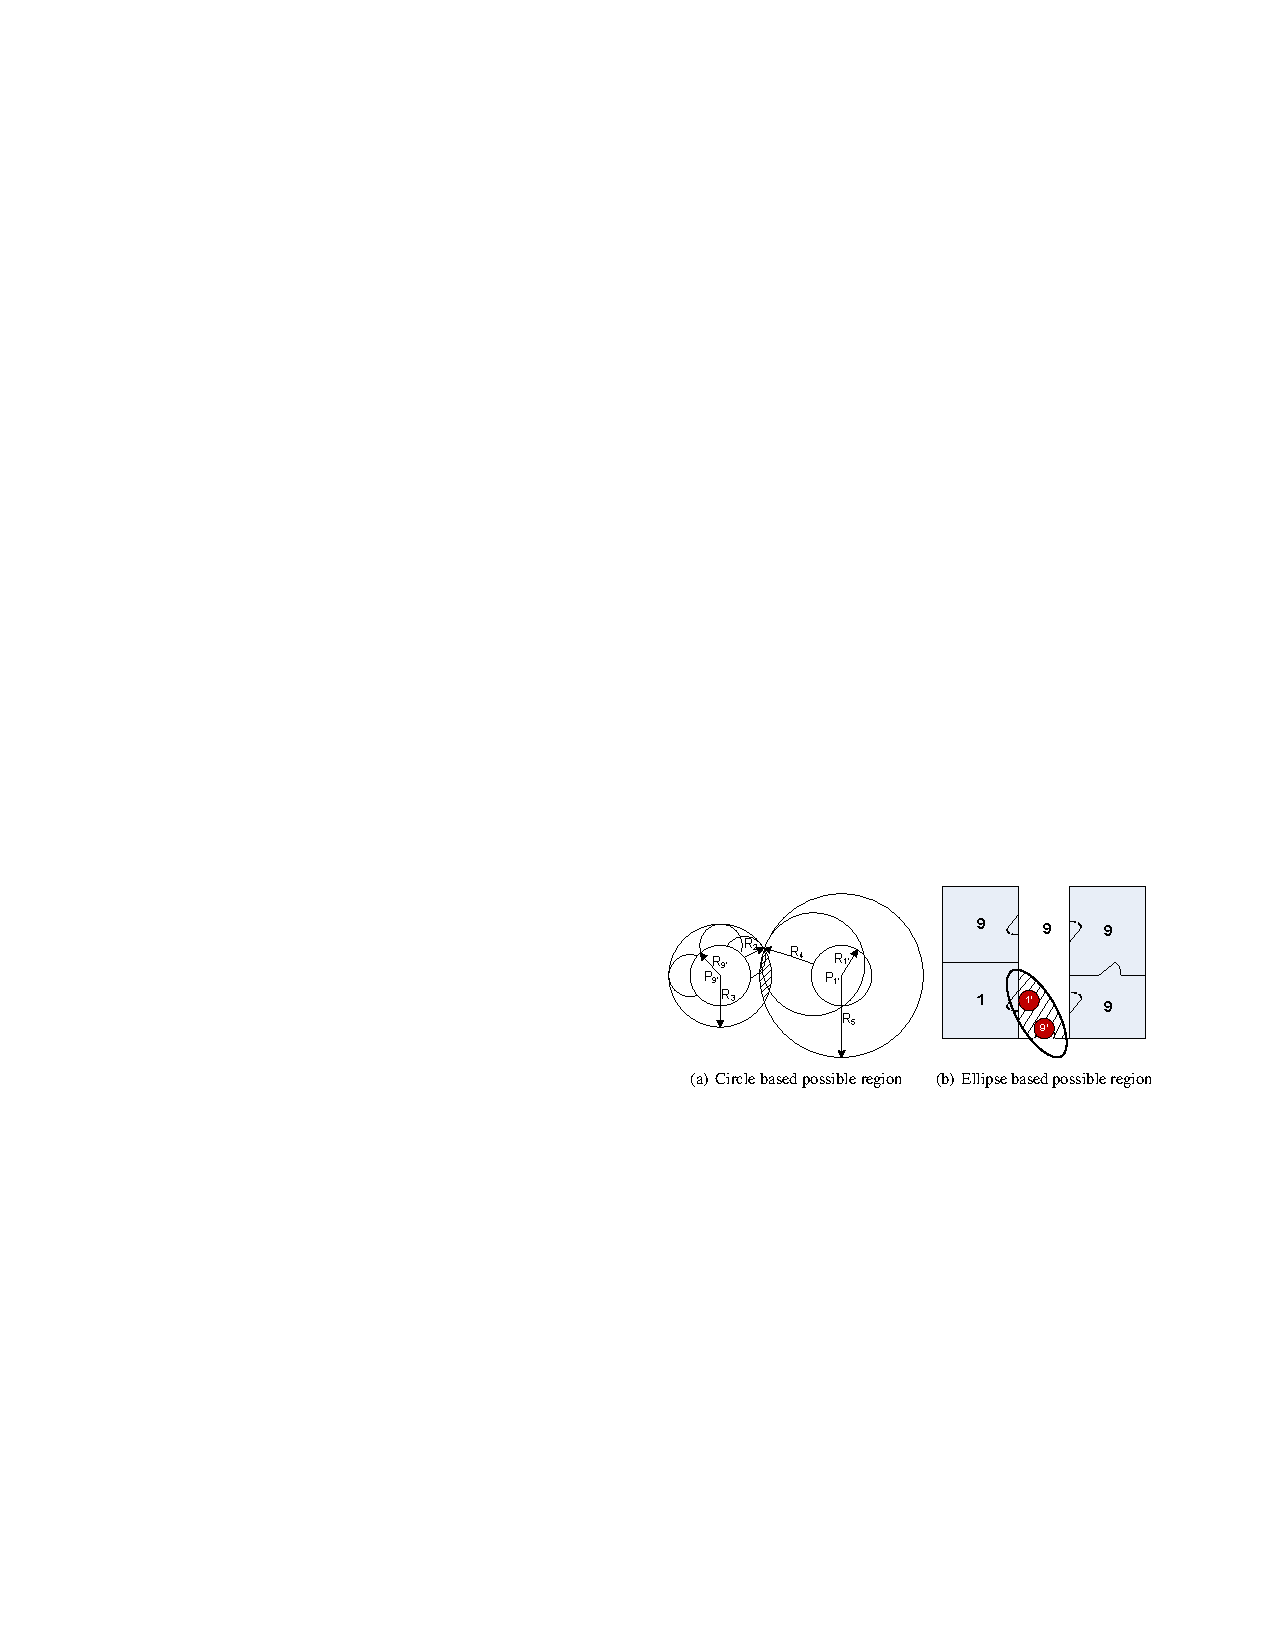
\includegraphics[width=\columnwidth]{figures/2-1/2-1-12.pdf}
\end{figure}
\tiny{
  \pause
  $\left.\begin{matrix}
  \mn{(reading_1, reader_{9}, tag_1, t_1, t_2)}~~\\
  \mn{(reading_2, reader_{9'}, tag_1, t_3, t_4)}~~\\
  \mn{(reading_3, reader_{1'}, tag_1, t_7, t_8)}~~\\
  \mn{(reading_4, reader_{1}, tag_1, t_9, t_10)}~~
  \end{matrix}\right\} \overset{Step~1}{\rightarrow} \pause$ \\~\\~\\

  $\left.\begin{matrix}
  \mn{(tag_1, [t_1,t_4], e\langle 10,9 \rangle, reader_{9}, reader_{9'})}~~\\
  \mn{(tag_1, [t_7,t_{10}], e\langle 9,1 \rangle, reader_{1'}, reader_{1})}~~
  \end{matrix}\right\} \overset{Step~2}{\rightarrow} \pause$ \\~\\~\\

  $\mn{(tag_1, [t_5,t_6], c_9, reader_{9'}, reader_{1'})} \overset{Step~3}{\rightarrow} \pause$ \\~\\~\\

  $\mn{(tag_1, [t_5,t_6], c_9 \cup \Theta(reader_{9'}, reader_{1'}, t_5, t_6))}$
}

\end{columns}

\end{frame}

%------------------------------------------------

\begin{frame}
\frametitle{On-line Tracking}

\small{\textrm{Given $\mn{\langle readerID, tagID, t, flag \rangle}$. \conceptbf{On-line tracking} is intended to infer the trajectory in the time interval between the last observation and the current time or even in the future.}}
\\~\\

\begin{columns}[c]

  \column{.35\textwidth}
  \begin{figure}[tb]
    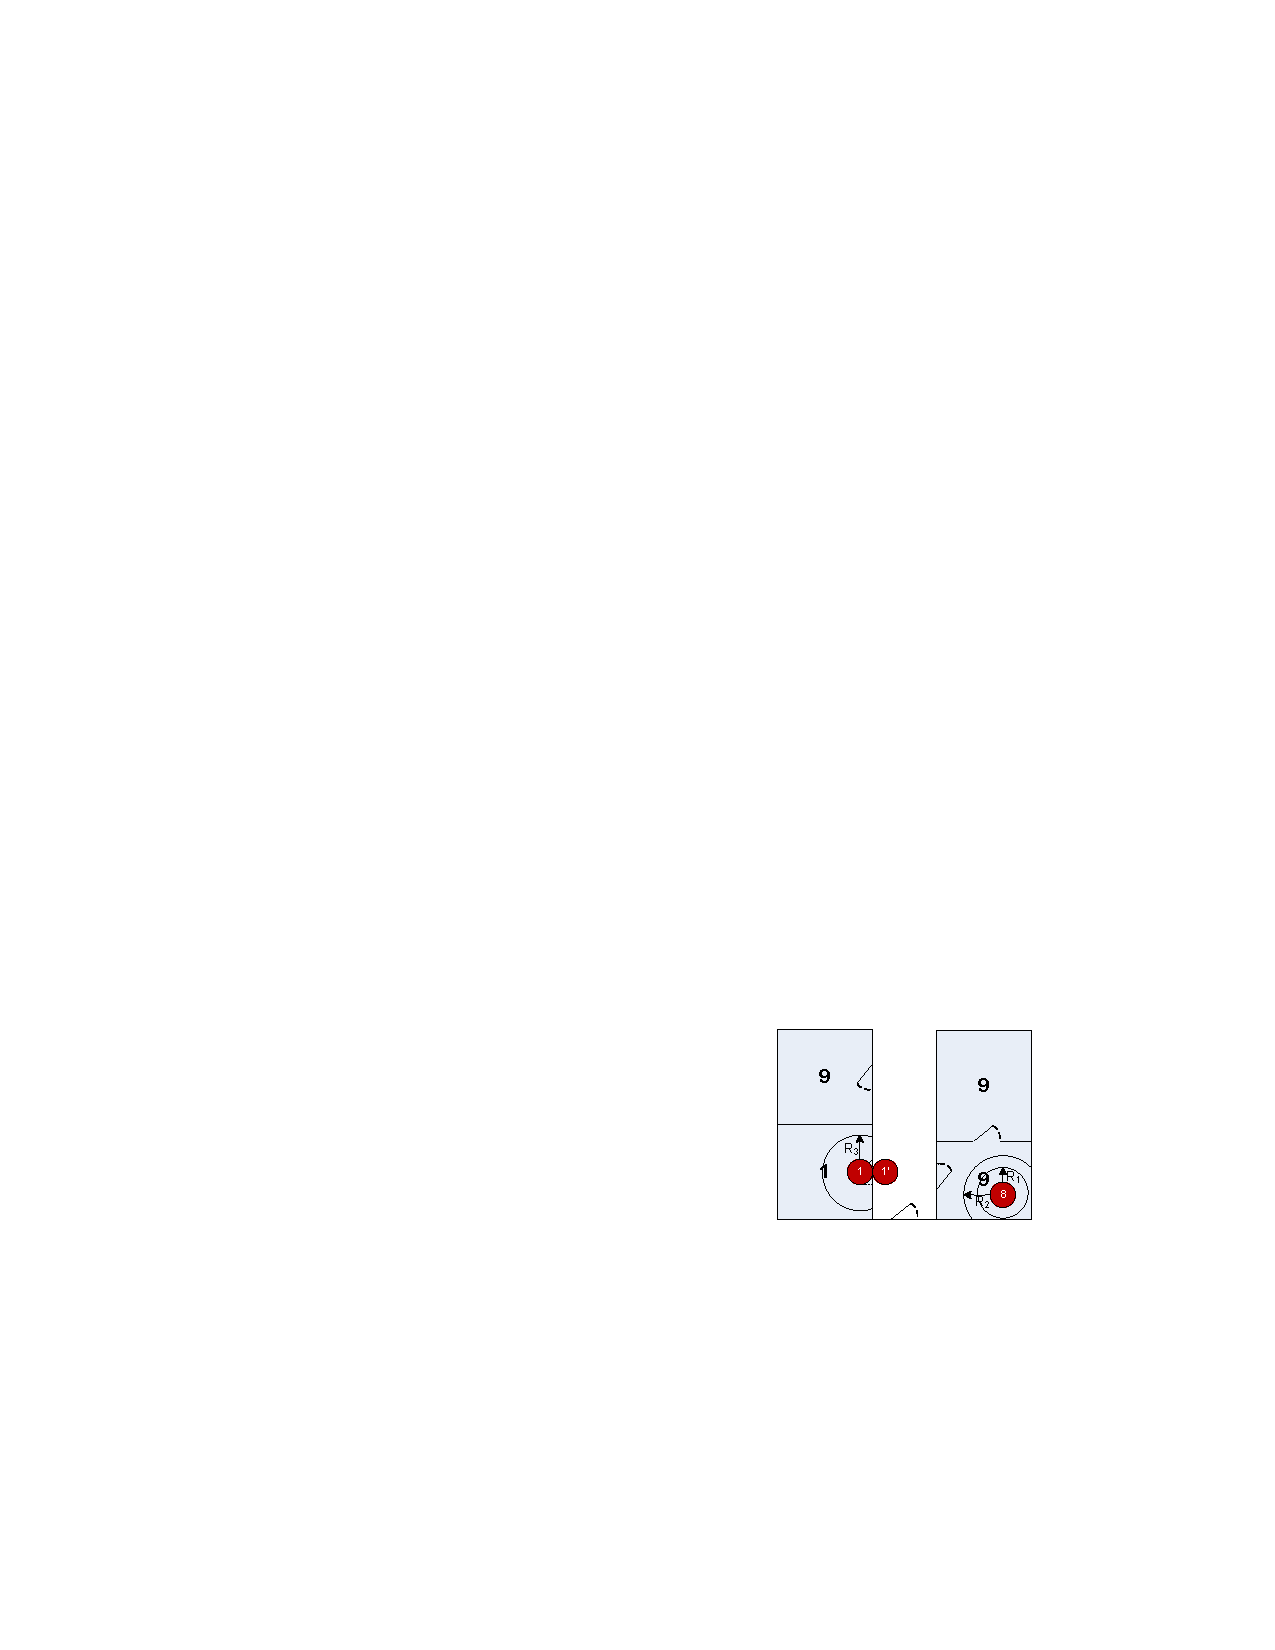
\includegraphics[width=\columnwidth]{figures/2-1/2-1-13.pdf}
  \end{figure}


  \column{.65\textwidth}
  \fsize{
    \begin{itemize}
      \item $\mn{flag = START}$, object $\mn{tagID}$ is in the activation range of $\mn{readerID}$ at time $\mn{t}$.
      \item $\mn{flag = END}$, the object is beyond the activation range of $\mn{readerID}$ and not in the range of any other readers.
				\begin{itemize}
					\ssize{
					\item constrains by a circle determined by the most recent observing reader's range.
					\item further refined if an object has recently been detected by a partitioning reader pair.
					}
				\end{itemize}
    \end{itemize}
  }

\end{columns}

\end{frame}

%------------------------------------------------

\begin{frame}
\frametitle{Research Directions}

\begin{itemize}
	\item Extend the deployment graphs to accommodate RFID readers with large and overlapping activation ranges. \\~\\
	\item Using multiple deployment graphs for several positioning technologies. \\~\\
	\item To enhance on-line tracking. Historical data $\rightarrow$ association rules $\rightarrow$ better prediction.
\end{itemize}

\end{frame}


\subsection{2.2 Scalable Continuous Range Monitoring of Moving Objects in Symbolic Indoor Space} % A subsection can be created just before a set of slides with a common theme to further break down your presentation into chunks

%\begin{frame}
\frametitle{About This Work...}

\emph{Scalable Continuous Range Monitoring of Moving Objects in Symbolic Indoor Space}.~\cite{DBLP:conf/cikm/YangLJ09} \\
B.~Yang, H.~Lu, and C.~S. Jensen.\\~\\

\begin{itemize}
  \item Published in \emph{CIKM' 2009}.
\end{itemize}

\end{frame}

%------------------------------------------------


\subsection{2.3 Probabilistic Threshold k Nearest Neighbor Queries over Moving Objects in Symbolic Indoor Space} % A subsection can be created just before a set of slides with a common theme to further break down your presentation into chunks

\begin{frame}
\frametitle{About This Work...}

\emph{Probabilistic Threshold $k$ Nearest Neighbor Queries over Moving Objects in Symbolic Indoor Space}.~\cite{DBLP:conf/edbt/YangLJ10} \\
B.~Yang, H.~Lu, and C.~S. Jensen.\\~\\

\begin{itemize}
  \item Published in year 2010 at the \emph{EDBT} conference.
  \item \emph{Minimal Indoor Walking Distance}(MIWD) along with algorithms and data structures are proposed for distance computing and storage.
  \item Effective object indexing structures, also capture the uncertainty of object locations.
  \item On this foundation, Probabilistic threshold $k$NN (PT$k$NN) query is studied.
\end{itemize}

\end{frame}
%------------------------------------------------

\begin{frame}
\frametitle{Motivation}

\begin{itemize}
  \item Indoor positioning makes it possible to support interesting queries over large populations of moving objects.
    \begin{itemize}
      \item shopping mall, airports, office buildings
      \item $k$NN queries over indoor moving objects enables the detection of approaching potential threats at sensitive locations in a subway system
    \end{itemize}
  \\~\\
  \item Existing $k$NN techniques in spatial and spatialtemporal databases are inapplicable in indoor spaces.
    \begin{itemize}
      \item complex entities and topologies
      \item indoor positioning techniques differ fundamentally from outdoor GPS, low sampling frequency and accuracy
    \end{itemize}
\end{itemize}

\end{frame}
%------------------------------------------------


\subsection{2.4 Spatio-temporal Joins on Symbolic Indoor Tracking Data} % A subsection can be created just before a set of slides with a common theme to further break down your presentation into chunks

%\begin{frame}
\frametitle{About This Work...}

\emph{Spatio-temporal Joins on Symbolic Indoor Tracking Data}.~\cite{DBLP:conf/icde/LuYCJ11} \\
H.~Lu, B.~Yang, and C.~S. Jensen.\\~\\

\begin{itemize}
  \item Published at \emph{ICDE' 2011}.
  \item Studies the probabilistic, spatio-temporal joins on hisorical indoor tracking data.
  \item Two-phase hash-based algorithms are proposed for the point and interval joins.
  \item A filter-and-refine framework, along with spatial indexes and pruning rules.
\end{itemize}

\end{frame}
%------------------------------------------------

\begin{frame}
\frametitle{Motivation}

\begin{itemize}
  \item Huge amount of tracking data serves as a foundation for a wide variety of indoor applications and services.\cite{jensen2010indoor}
    \begin{fitemize}
      \item shopping mall, airports, office buildings, akin to those enabled by outdoor GPS
      \item hot area detection, space planning, security control, movement pattern discovery
    \end{fitemize}

  \item Spatio-temporal joins fall short in indoor setting.
    \begin{fitemize}
      \item indoor space consists of semantic entities enable or constrain movement
      \item semantics of indoor space call for novel spatio-temporal join predicates
      \item indoor positioning technologies differ fundamentally from outdoor setting, low accuracy and sampling frequency
    \end{fitemize}

  \item Joins on indoor tracking data call for new definition and new implementation techniques that take into account:
  \begin{fitemize}
    \item specifics of indoor space
    \item limitations of indoor positioning
  \end{fitemize}
\end{itemize}

\end{frame}
%------------------------------------------------

%------------------------------------------------

\begin{frame}
\frametitle{Preliminaries: Symbolic Indoor Tracking}

\begin{figure}[tb]
  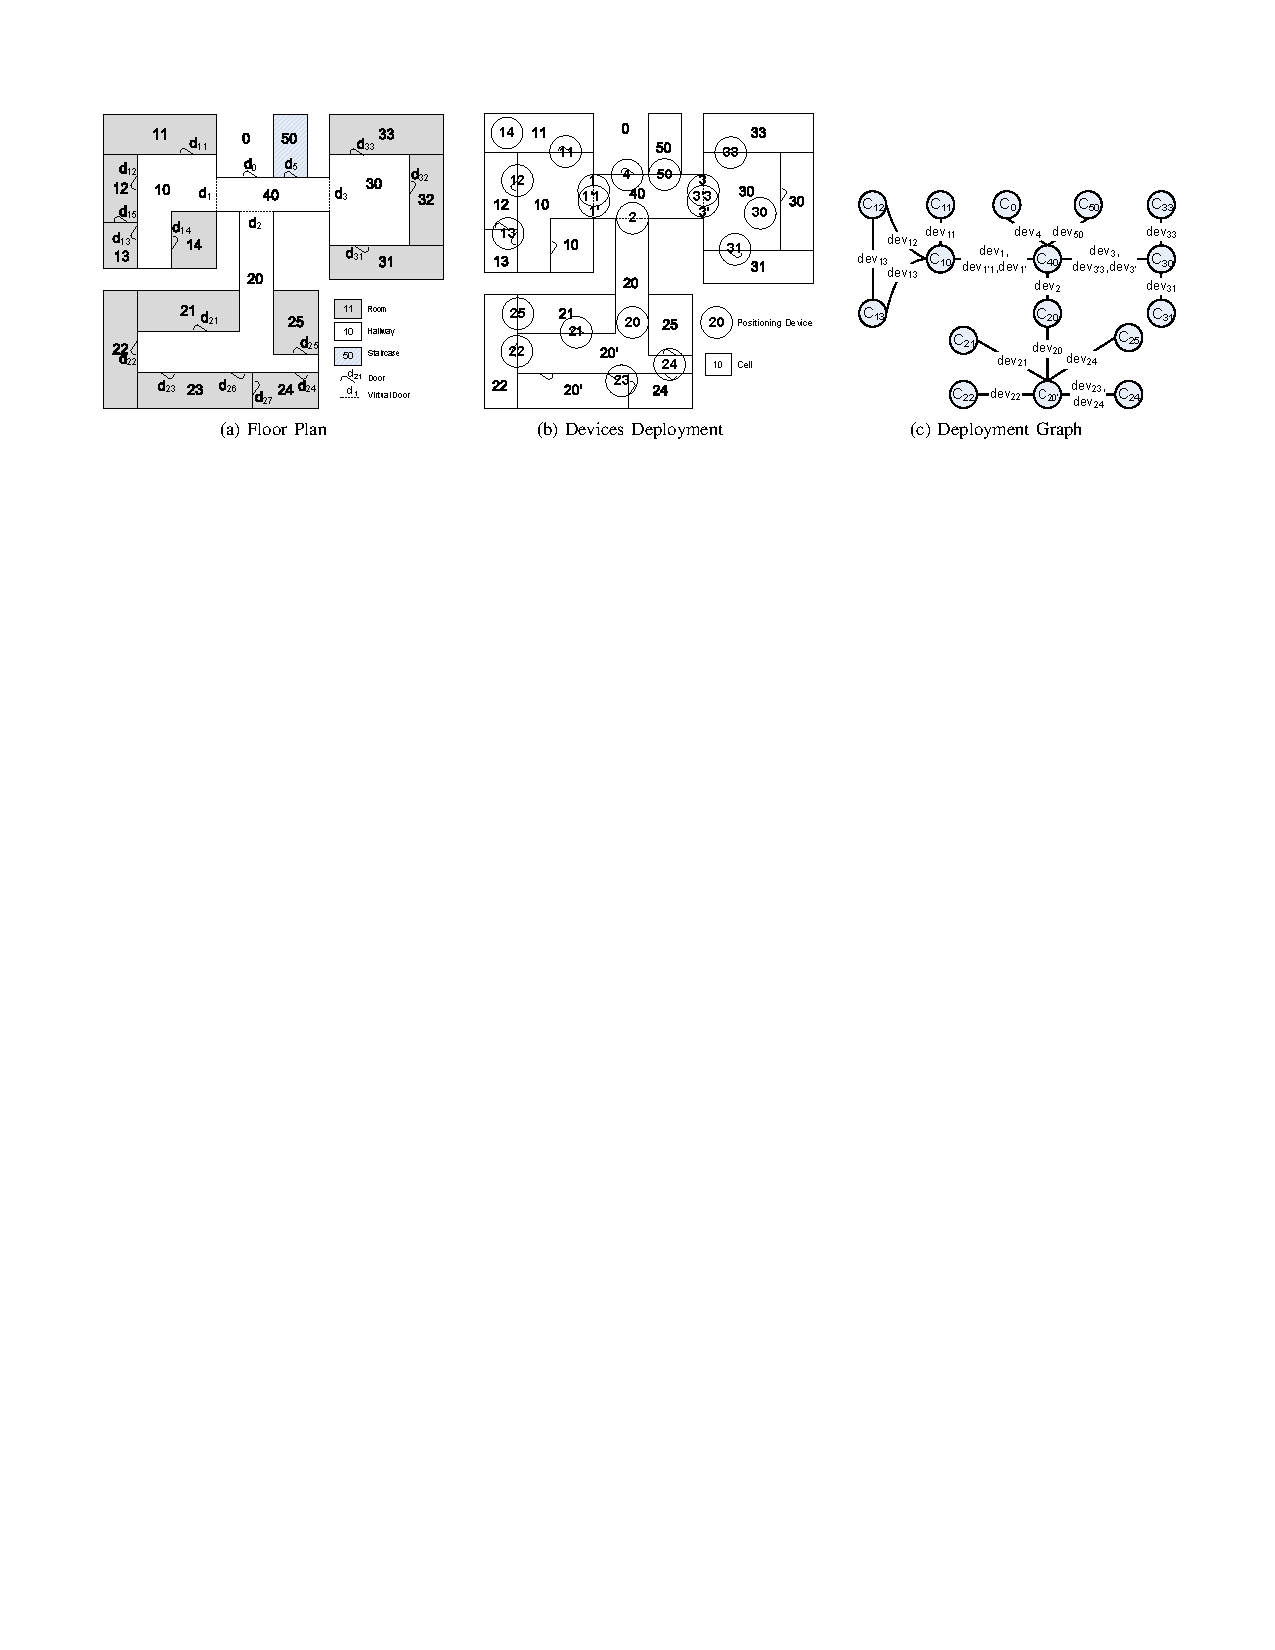
\includegraphics[width=\columnwidth]{figures/2-4/2-4-1.pdf}
\end{figure}

\begin{enumerate}
  \ssize{
  \item $\mn{C2P: C \rightarrow 2^P}$ maps a cell to a set of indoor partitions
  \item $\mn{D2C: D \rightarrow 2^C}$ maps a device to a set of corresponding cells
  \item According to Deployment Graph, for partitioning device, $\mn{D2C(device_{13})} = \{ C_{10},C_{13} \} \cup \{ C_{12},C_{13} \} = \{ C_{10},C_{12},C_{13} \}$
  \item For presence device, $\mn{D2C(device_{25})} = \{ C_{21},C_{22} \}$ as the cells intersect its detection range.
  \item $\mn{D2C: D \rightarrow 2^C}$ is useful as it captures the possible movements of objects.
  }
\end{enumerate}

\end{frame}

%------------------------------------------------

\begin{frame}
\frametitle{Preliminaries: Symbolic Indoor Tracking}

\begin{columns}[c]
  \column{.52\textwidth}
  \begin{figure}[tb]
    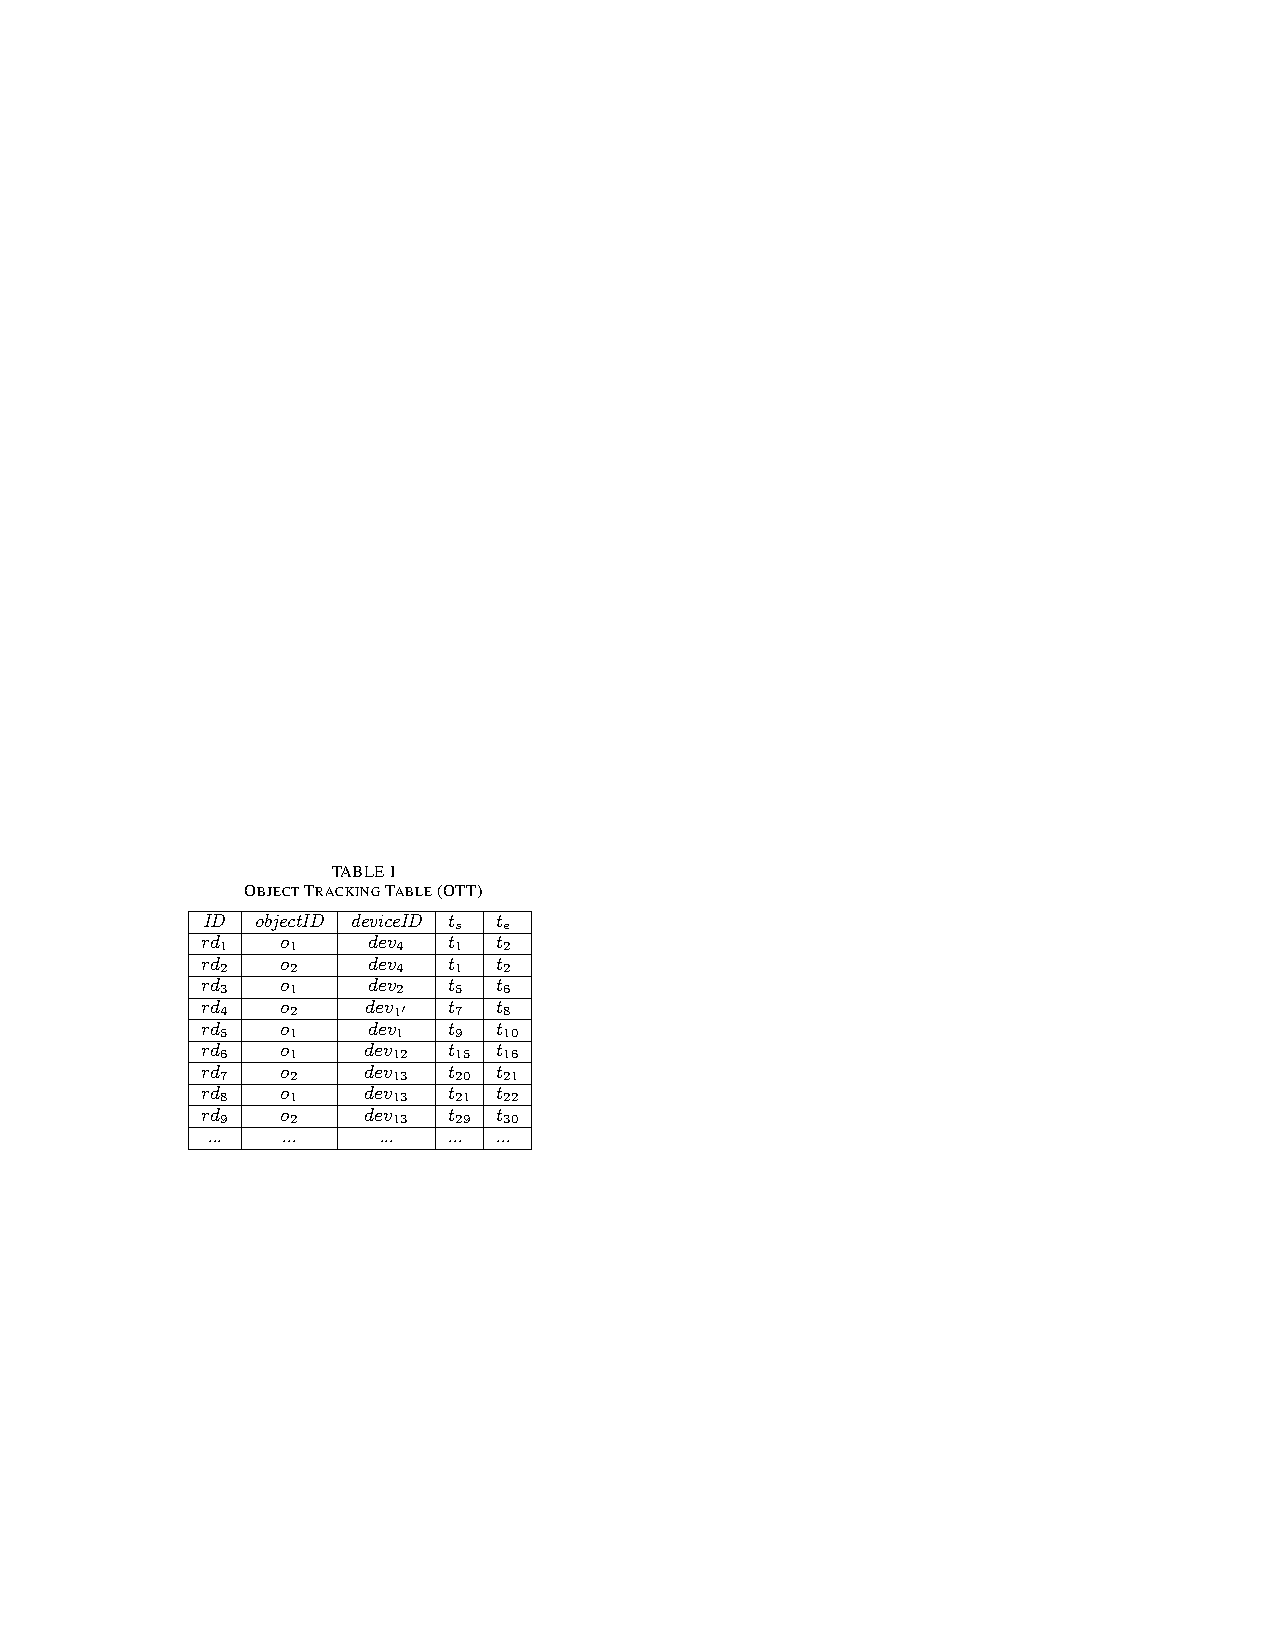
\includegraphics[width=\columnwidth]{figures/2-4/2-4-2.pdf}
  \end{figure}

  \column{.48\textwidth}
  \begin{fitemize}
    \item \conceptbf{Object Tracking Table} $\mn{OTT}$ records the converted trajectories with schema $\mn{(ID, objectID, deviceID, t_s, t_e)}$
    ~\\
    \item a record states that the object $\mn{objectID}$ is observed by the device $\mn{deviceID}$ in the closed interval from time $\mn{t_s}$ to $\mn{t_e}$.
  \end{fitemize}

\end{columns}

\end{frame}

%------------------------------------------------

\begin{frame}
\frametitle{Problem Definitions}

Given an $\mn{OTT}$, it is of interesting to identify object pairs that join w.r.t some specific spatio-temporal join predicate.
\begin{fitemize}
  \item to know all pair of individuals that were probably at the same gate when a particular event (terrorist attack) occurred in a large airport.
\end{fitemize}
~\\
Due to tracking uncertainty, only interested in those objects that satisfy the join predicate with some given probability (specified threshold).
\\~\\
The joins are effectively \emph{self-joins} because all tracking data is contained in a single $\mn{OTT}$.

\end{frame}

%------------------------------------------------

\begin{frame}
\frametitle{Problem Definition I}

\textrm{One can apply a join predicate to a time point to find pairs that join at that particular time point...}
\\~\\
\begin{definition}[\ssize{Probabilistic Threshold Indoor Spatio-temporal Join--PTISSJ}]
  \textrm{
  \ssize{
  Given an $\mn{OTT}$, a join predicate $\mn{P}$, a time point $\mn{t}$, and a threshold value $\mn{M \in (0,1]}$, a probabilistic threshold indoor spatio-temporal join  $\mn{\Join_{P,t,M}(OTT) = \{ (o_i, o_j) | o_i, o_j \in O  \wedge o_i \neq o_j \wedge pr(P(o_i, o_j, t)) >M \}}$, where $\mn{pr(P(o_i,o_j,t))}$ is the \textbf{Timeslice Join Probability} of $\mn{o_i, o_j}$ at time $\mn{t}$, i.e., the probability that predicate $\mn{P(o_i,o_j,t)}$ is true.
  }}
\end{definition}

\end{frame}

%------------------------------------------------

\begin{frame}
\frametitle{Problem Definition II}

\textrm{It's also interesting to know object pairs satisfy the predicate for some consecutive timestamp...}
\\~\\
\begin{definition}[\ssize{Probabilistic Threshold $k$ Indoor Spatio-temporal Join--PT$k$ISSJ}]
  \textrm{
  \ssize{
  Given an $\mn{OTT}$, a join predicate $\mn{P}$, a time interval $\mn{I = [t_m, t_n] (m < n)}$, an integer $\mn{k(0 < k \leq n - m)}$, and a threshold value $\mn{M \in (0,1]}$, a probabilistic $\mn{k}$ threshold indoor spatio-temporal join
  \begin{equation*}
    \begin{split}
    &\mn{\Join_{P,I,k,M}(OTT) = \{ (o_i, o_j) | o_i, o_j \in O \wedge o_i \neq o_j \wedge } \\
    &\mn{\exists s \in m...n -k + 1 (\forall\delta \in 0...k-1 (pr(P(o_i, o_j, t_{s+\delta})) > M)) \} }
    \end{split}
  \end{equation*}
  }}
\end{definition}

\end{frame}

%------------------------------------------------

\begin{frame}
\frametitle{Uncertainty Model for Indoor Tracking}

\textrm{For outdoor moving objects~\cite{cheng2004querying}, \conceptbf{Uncertainty Region}, denoted by $\mn{UR(o_i,t)}$, is a region such that $\mn{o_i}$ must be in this region at time $\mn{t}$.}\\~

In general terms, an object $\mn{o_i}$'s location can be modeled as a random variable $\mn{l}$ associated with a probability density function $\mn{f_{o_i}(l,t)}$ that has non-zero values only in $\mn{o_i}$'s suncertainty region $\mn{UR(o_i, t)}$.~\cite{DBLP:conf/edbt/YangLJ10}

\begin{equation}
  \mn{\int_{l \in UR(o_i,t)} f_{o_i}(l,t) dl = 1}
\end{equation}

\end{frame}

%------------------------------------------------

\begin{frame}
\frametitle{Object State in OTT}

\begin{columns}[c]

\column{.45\textwidth}
\begin{figure}[tb]
  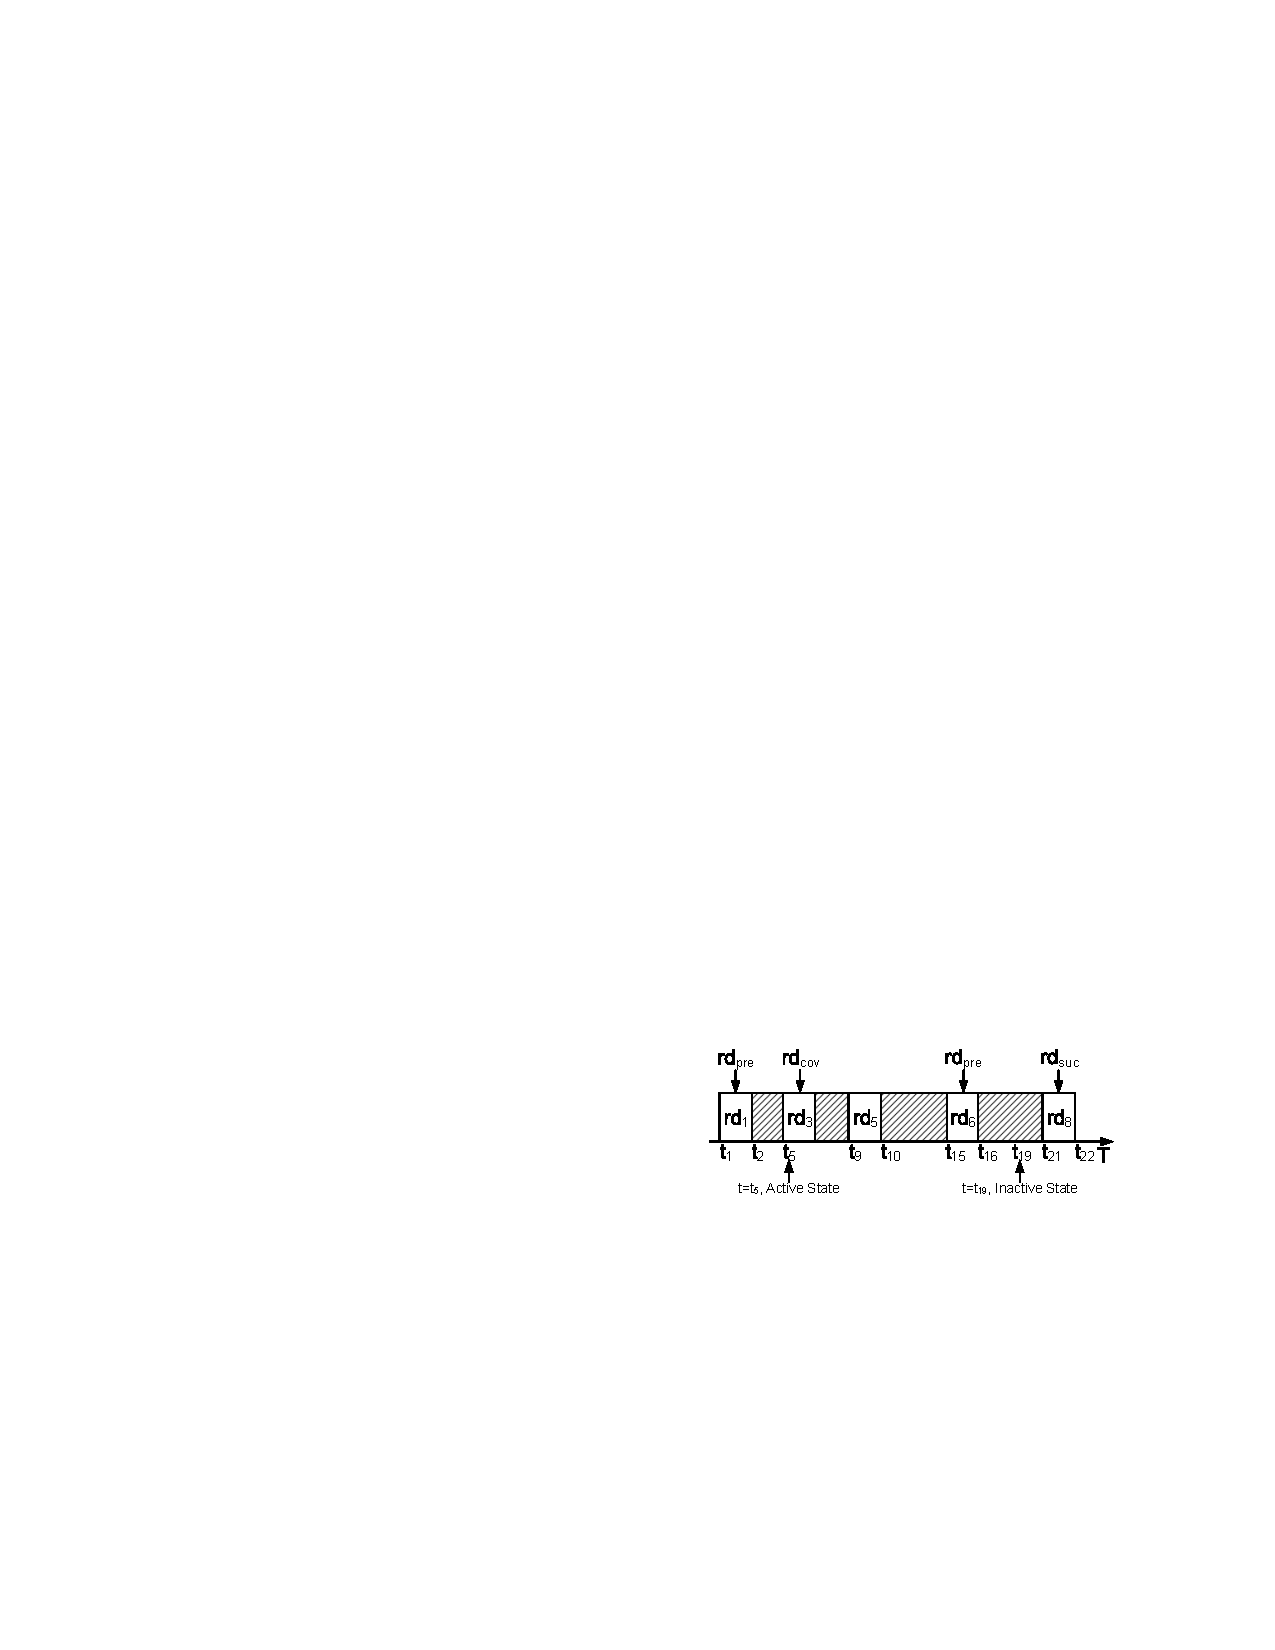
\includegraphics[width=\columnwidth]{figures/2-4/2-4-3.pdf}
\end{figure}

\column{.55\textwidth}
\begin{definition}[Active State]
  \textrm{
  \ssize{
  Given an object $\mn{o_i}$ and a time point $\mn{t}$, if a tracking record $\mn{rd_{cov}}$ is found in $\mn{OTT}$ such that $\mn{rd_{cov}.objectID = o_i}$ and $\mn{t \in [rd_{cov}.t_s, rd_{cov}.t_e]}$, $\mn{o_i}$ is in the \conceptbf{active state} at time $\mn{t}$.
  }}
\end{definition}

\end{columns}

\begin{definition}[Inactive State]
  \textrm{
  \ssize{
  Given an object $\mn{o_i}$ and a time point $\mn{t}$, if no record $\mn{rd_{cov}}$ is found in $\mn{OTT}$, $\mn{o_i}$ is in the \conceptbf{inactive state} at time $\mn{t}$. Instead, two tracking records of $\mn{o_i}$ called $\mn{rd_{pre}}$ and $\mn{rd_{suc}}$, can be found in $\mn{OTT}$, such that they are consecutive in the sense that $\mn{rd_{pre}.t_e < t < rd_{suc}.t_s}$ and there is no record for $\mn{o_i}$ between times $\mn{rd_{pre}.t_e}$ and $\mn{rd_{suc}.t_s}$.
  }}
\end{definition}

\end{frame}

%------------------------------------------------

\begin{frame}
\frametitle{Uncertainty Region in the Active State}

\begin{columns}[c]
  \column{.52\textwidth}
  \vspace{-10pt}
  \begin{figure}[tb]
    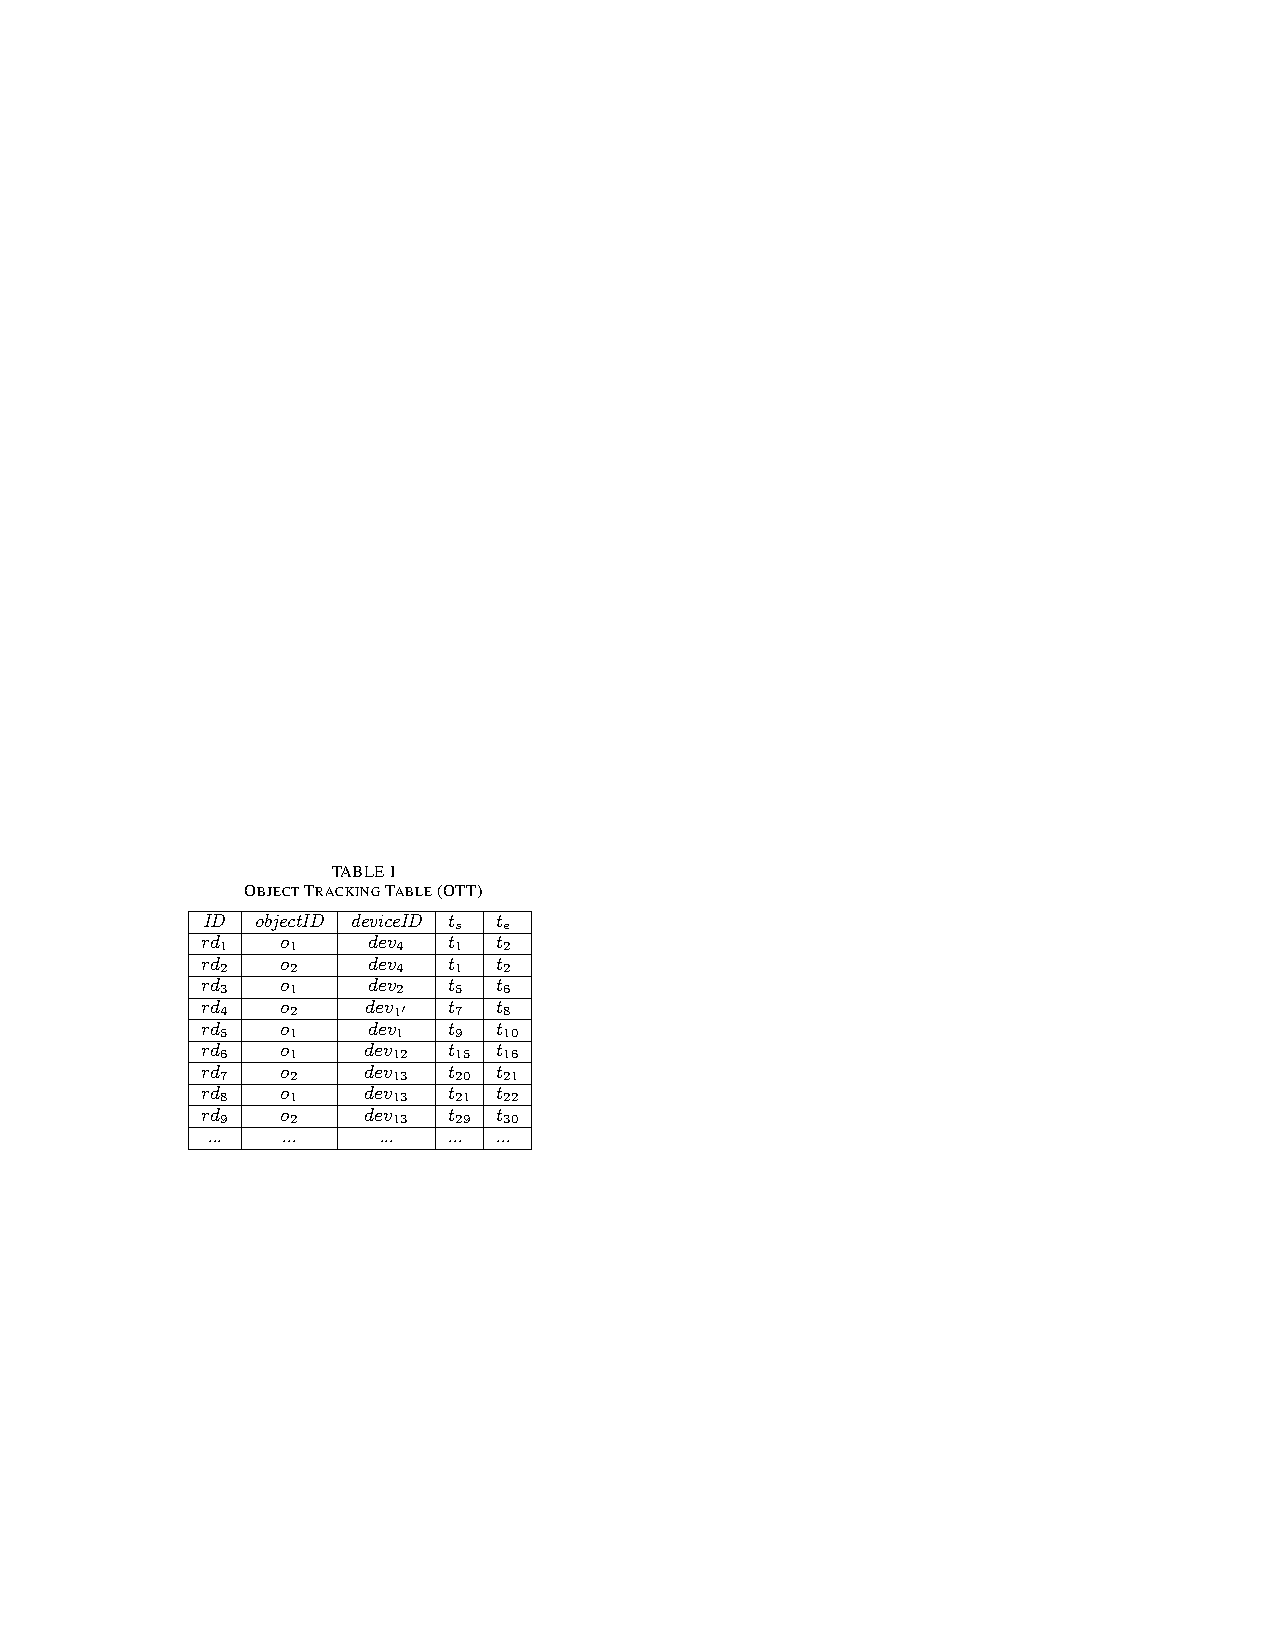
\includegraphics[width=\columnwidth]{figures/2-4/2-4-2.pdf}
  \end{figure}
  \vspace{-15pt}
  \begin{example}
    \textrm{
    \ssize{
    $\mn{t = t_5}$, $\mn{rd_{cov} = rd_3}$ and $\mn{rd_{pre} = rd_1}$, which tells $\mn{o_i}$ left $\mn{dev_4}$'s detection range at time $\mn{t_2}$, and is currently detected by $\mn{dev_2}$.
    }}
  \end{example}

  \column{.48\textwidth}
  \vspace{-10pt}
  \begin{figure}[tb]
    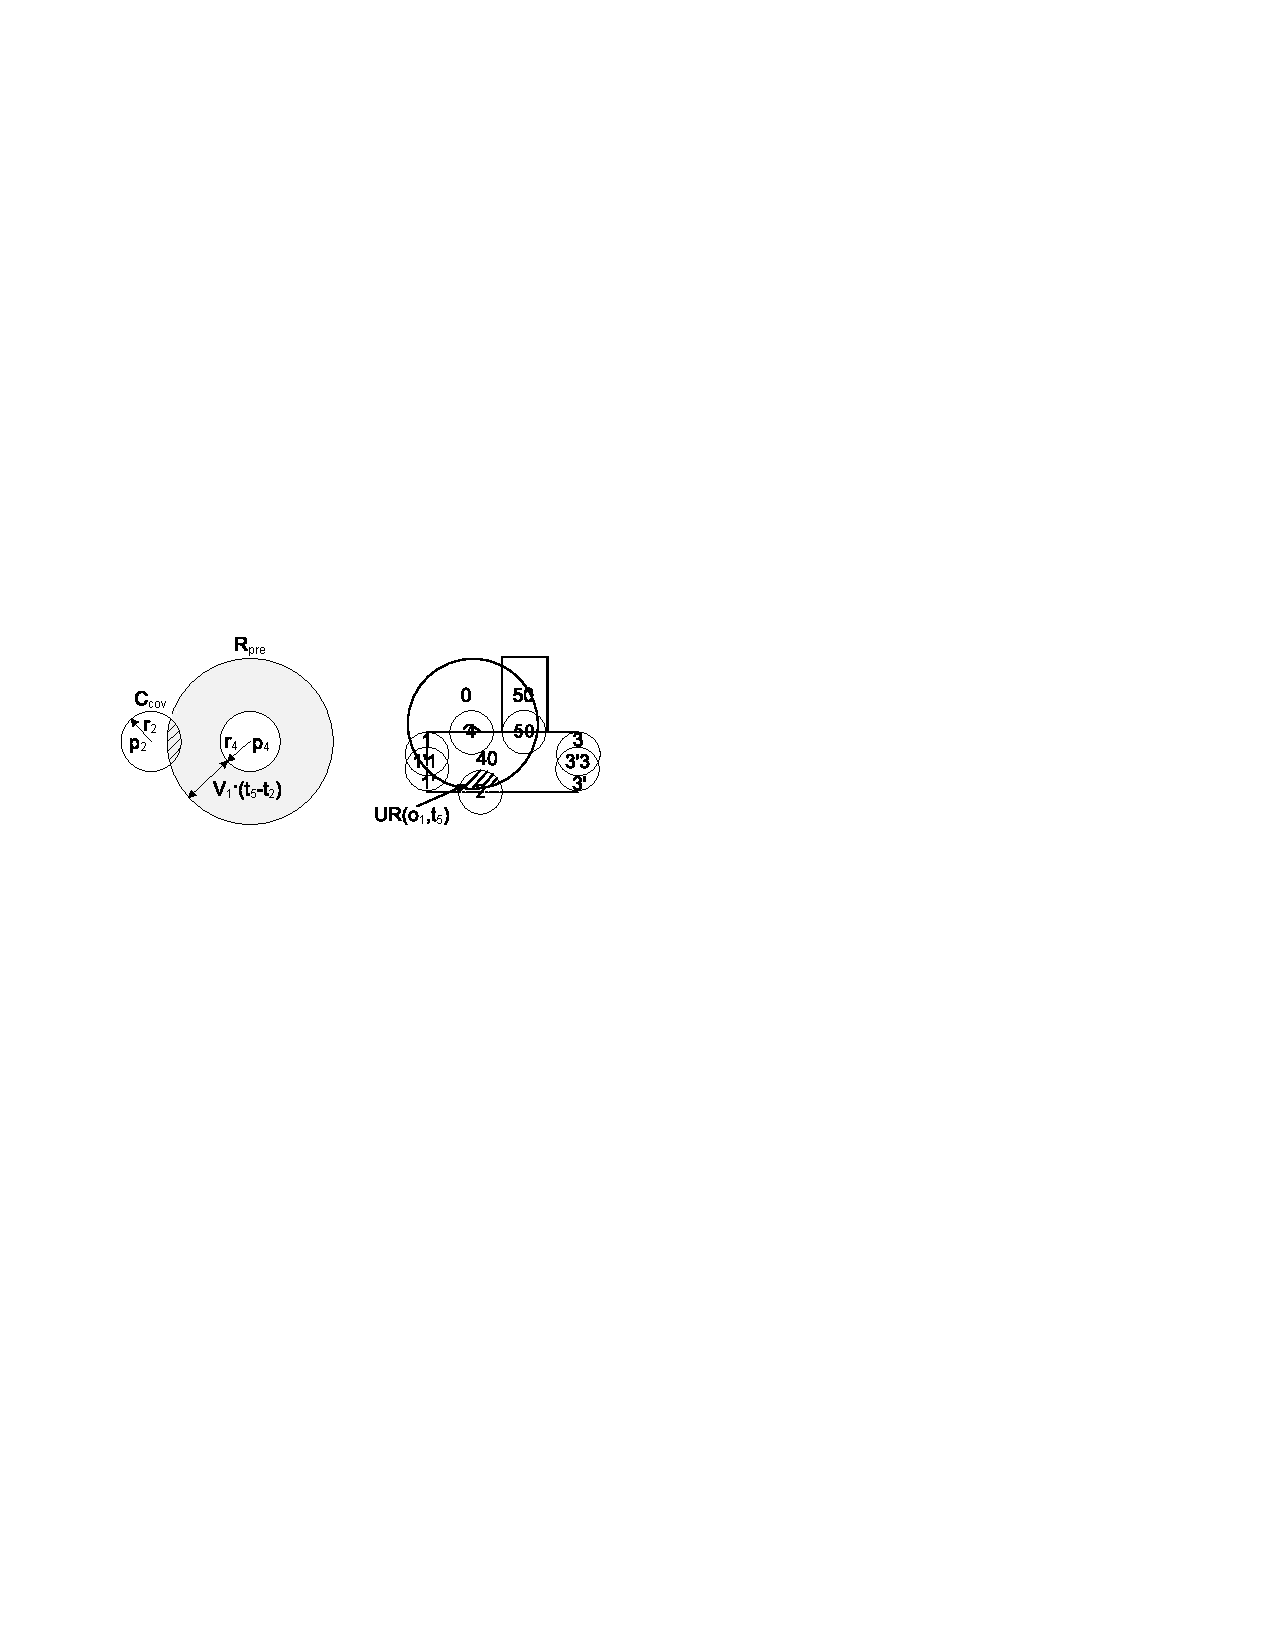
\includegraphics[width=\columnwidth]{figures/2-4/2-4-4.pdf}
  \end{figure}
  \ssize{
  \textbf{Step 1:}
  UR is the detection range of device $\mn{rd_{cov}.deviceID}$, denote as:
  \begin{equation*}
  \begin{split}
    \mn{ C_{cov} = } &\mn { Cir(Loc(rd_{cov}.deviceID), }\\
    &\mn{ Rad(rd_{cov}.deviceID)) }
  \end{split}
  \end{equation*}
  ~\\
  \textbf{Step 2:}
  UR should consider the $\mn{rd_{pre}}$'s \emph{maximum speed bounding ring}(MSBR):
  \tiny{
  \begin{equation*}
  \begin{split}
    &\mn{ UR(o_i, t) = C_{cov} \cap Ring(Loc(rd_{pre}.deviceID), } \\
    &\mn{ Rad(rd_{pre}.deviceID), V_i \cdot (t - rd_{pre}.t_e) ) }
  \end{split}
  \end{equation*}
  }
  }
\end{columns}

\end{frame}

%------------------------------------------------

\begin{frame}
\frametitle{Uncertainty Region in the Inactive State}

\begin{columns}[c]

  \column{.52\textwidth}
  \vspace{-10pt}
  \begin{figure}[tb]
    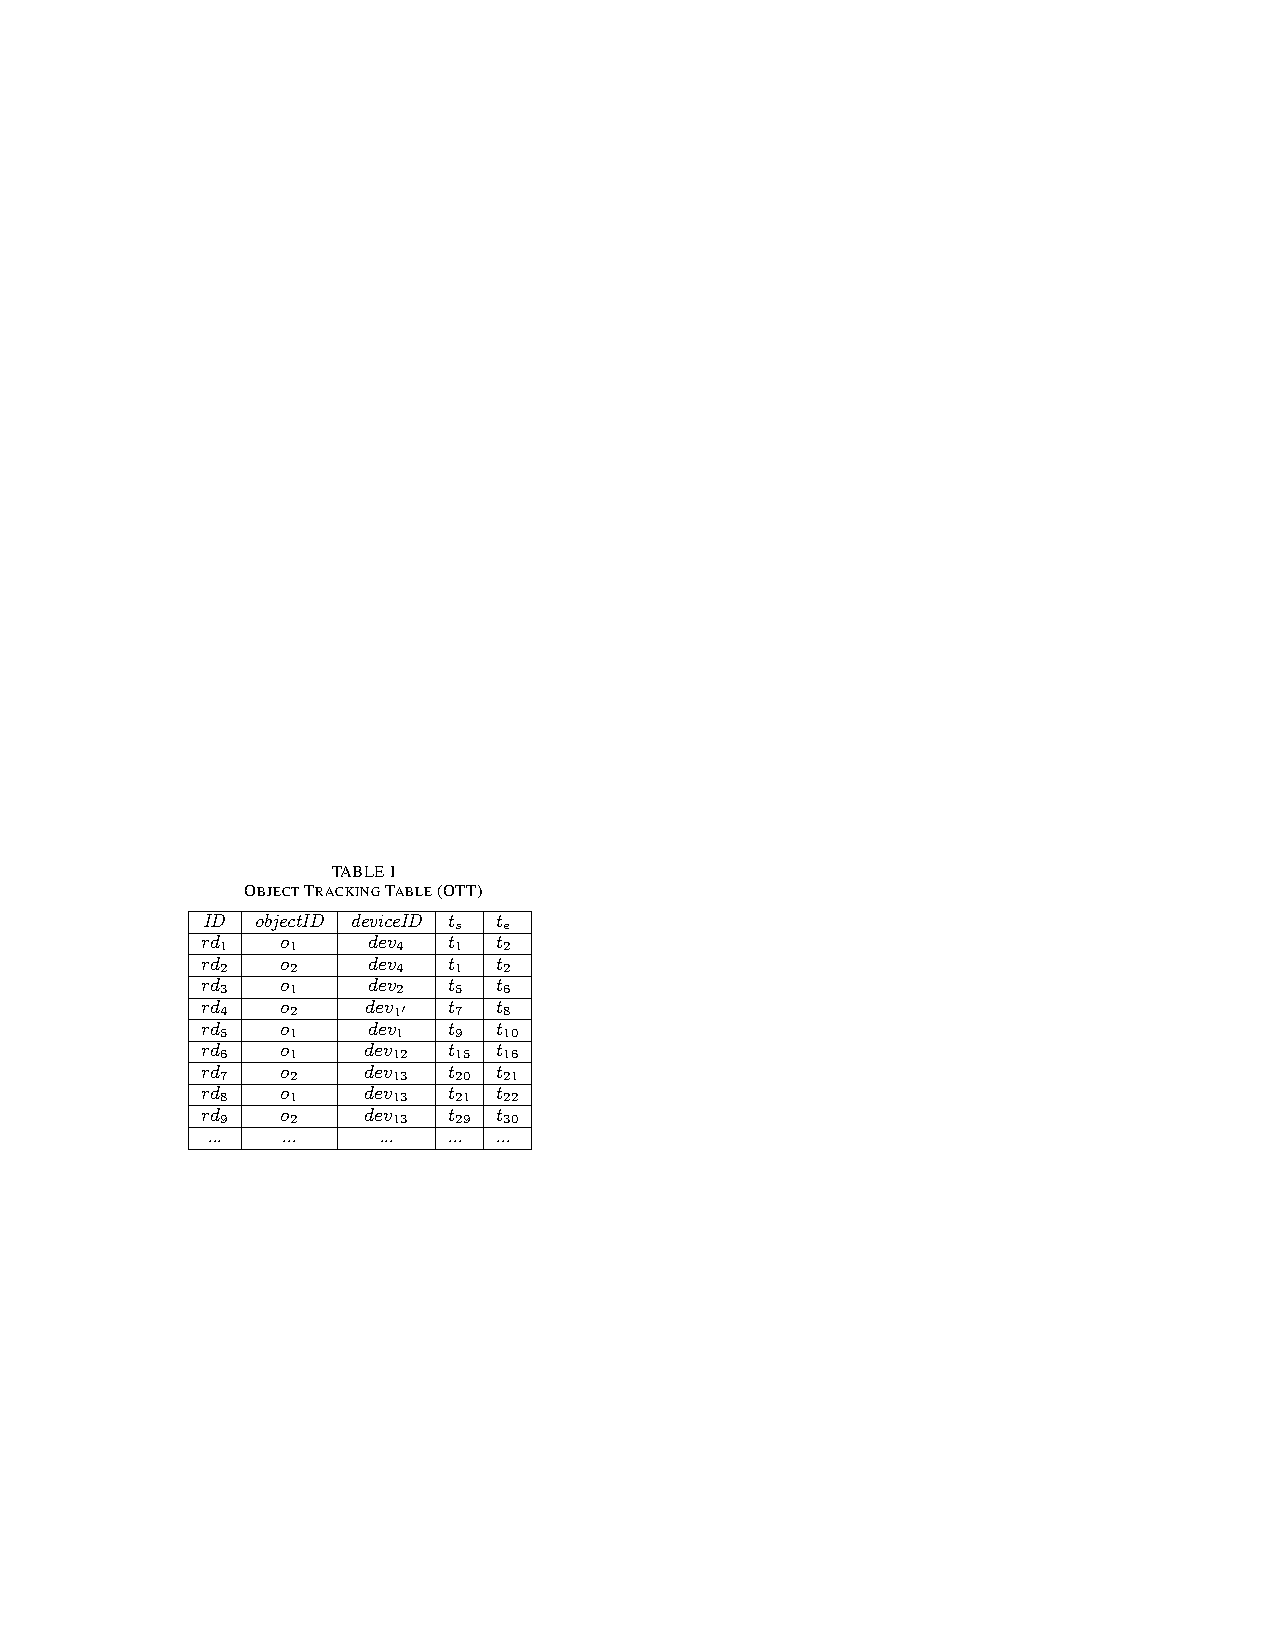
\includegraphics[width=\columnwidth]{figures/2-4/2-4-2.pdf}
  \end{figure}
  \vspace{-15pt}
  \begin{example}
    \textrm{
    \ssize{
    $\mn{t = t_{19}}$, $\mn{rd_{pre} = rd_6}$ and $\mn{rd_{suc} = rd_8}$, since $\mn{rd_6.t_e = t_{16} < t_{19} < rd_8.t_s = t_{21}}$. we have $\mn{dev_p = dev_{12}}$ and $\mn{dev_s = dev_{13}}$
    }}
  \end{example}

  \column{.48\textwidth}
  \vspace{-10pt}
  \begin{figure}[tb]
    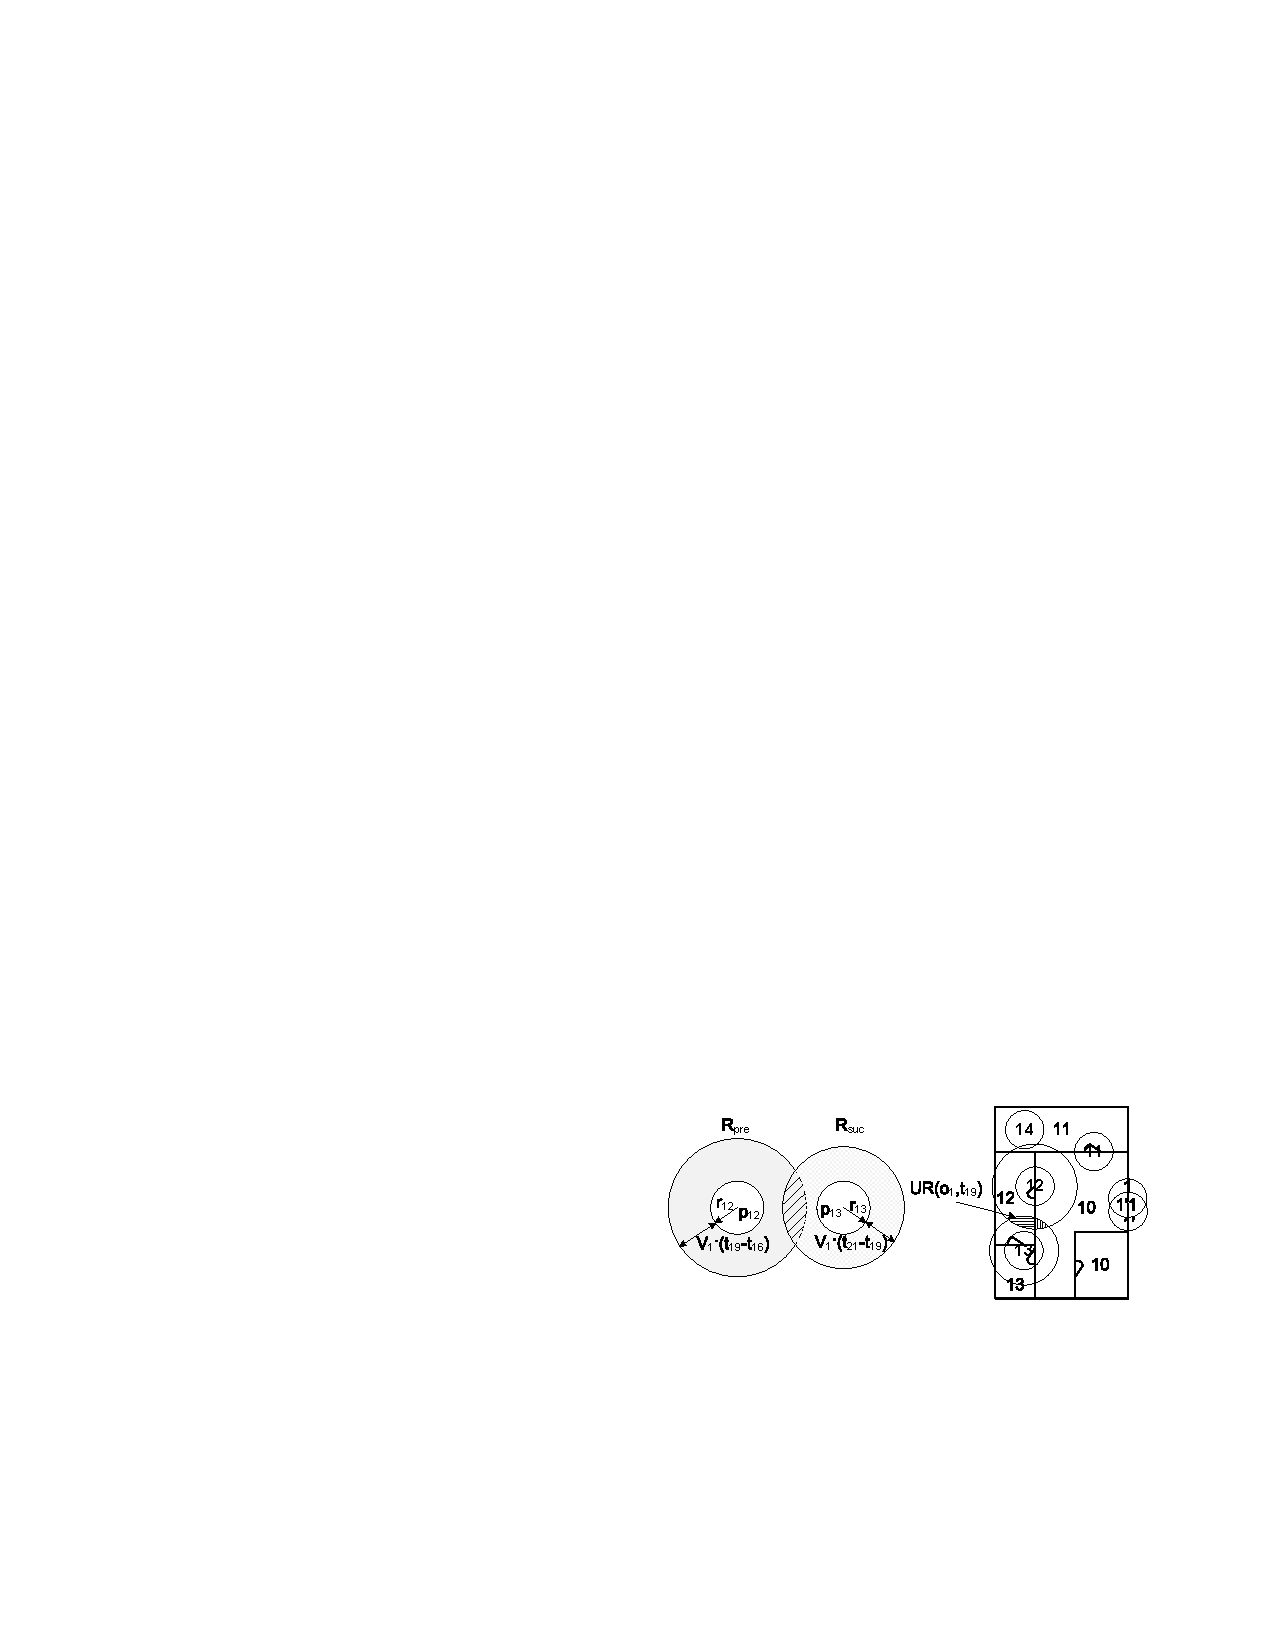
\includegraphics[width=\columnwidth]{figures/2-4/2-4-5.pdf}
  \end{figure}
  \ssize{
  \textbf{Step 1:}
  Determine the possible cells in which the object can be in the inactive period:
  \begin{equation*}
    \mn{ Cells_{mid} = D2C(dev_p) \cup D2C(dev_s)}
  \end{equation*}
  ~\\
  \textbf{Step 2:}
  UR is constrained by two \emph{maximum speed bounding ring}(MSBR)s of $\mn{rd_{pre}}$ and $\mn{rd_{suc}}$:
  \tiny{
  \begin{equation*}
  \begin{split}
    \mn{ UR(o_i, t) = \bigcup_{c \in Cells_{mid}} c \cap R_{pre} \cap R_{suc} }
  \end{split}
  \end{equation*}
  }
  }
\end{columns}

\end{frame}

%------------------------------------------------

\begin{frame}
\frametitle{Join Probability Evaluation}

\begin{definition}[the \emph{same X} predicate]
  \textrm{
  \ssize{
    termed as $\mn{P_X}$, where $\mn{X}$ represents an indoor region type. $\mn{IR_X}$ represents all $\mn{X}$ type regions ($\mn{X}$-regions).
  }
  }
\end{definition}
~\\
\begin{example}[the \emph{same room} predicate]
  \textrm{
  \ssize{
    Given two objects $\mn{o_i, o_j}$ at a time point $\mn{t}$, the \emph{same room} predicate $\mn{P_X(o_i, o_j, t)}$ evaluates to true if both $\mn{o_i, o_j}$ were located in a same room $\mn{rm \in IR_X}$. Other predicates can be \emph{same floor, same reserach group (maps to several rooms)}.
  }
  }
\end{example}
~\\
The \emph{same X} predicates are more practical than Euclidean distance based join predicates in indoor space.

\end{frame}

%------------------------------------------------

\begin{frame}
\frametitle{Join Probability Evaluation}
\vspace{-10pt}
\begin{definition}[``be located at'' predicate probability]
  \textrm{
  \ssize{
    Given an object $\mn{o_i}$, an $\mn{X}$-region $\mn{x_l \in IR_X}$, and a time $\mn{t}$, predicate $\Theta(o_i, x_l, t)$ indicate that $\mn{o_i}$ was located in $\mn{x_l}$ at $\mn{t}$. The probability that $\mn{\Theta}$ is satisfied is defined as:
    \begin{equation*}
      \mn{pr(\Theta(o_i, x_l, t)) = \frac{Area(UR(o_i, t) \cap x_l)}{Area(UR(o_i, t))}}
    \end{equation*}
  }
  }
\end{definition}

\begin{definition}[the \emph{same X} predicate probability]
  \textrm{
  \ssize{
    The probability that $\mn{o_i}$ and $\mn{o_j}$ were located in the same $\mn{x_l}$ at $\mn{t}$, indicated by $\mn{pr(P_{x_l}(o_i, o_j, t))}$ is defined as:
    \begin{equation*}
      \mn{pr(P_{x_l}(o_i, o_j, t)) = pr(\Theta(o_i, x_l, t)) \cdot pr(\Theta(o_j, x_l, t)) }
    \end{equation*}
    Therefore, the porbability that $\mn{o_i}$ and $\mn{o_j}$ satisfy a \emph{same X} predicate at time $\mn{t}$ can be defined as:
    \begin{equation*}
      \mn{pr(P_X(o_i, o_j, t)) = \max_{x_l \in IR_X} pr(P_{x_l}(o_i, o_j, t)) }
    \end{equation*}
  }
  }
\end{definition}

\end{frame}

%------------------------------------------------

\begin{frame}
\frametitle{Indexing the Indoor Tracking Data}

\textrm{to determine the \emph{Uncertainty Region} during join processing, it needs to retrieve the records $\mn{rd_{cov}}$ and $\mn{rd_{pre}}$ for active objects or $\mn{rd_{pre}}$ and $\mn{rd_{suc}}$ for inactive state.}
\\~\\
to index $\mn{OTT}$ with an augmented 1D R-tree, where each leaf entry has the form $\mn{(t^{\vdash},t^{\dashv},Ptr_{p},Ptr_{c})}$. $\mn{t^{\vdash} = rd_p.t_e}$, $\mn{t^{\dashv} = rd_c.t_e}$, $\mn{Ptr_p}$ and $\mn{Ptr_c}$ points to $\mn{rd_p}$ and $\mn{rd_c}$ respectively.

\begin{fitemize}
  \item if $\mn{t \geq rd_c.t_s}$, $\mn{o_i}$ is active, $\mn{rd_p \rightarrow rd_{pre}}$ and $\mn{rd_c \rightarrow rd_{cov}}$;
  \item if $\mn{t < rd_c.t_s}$, $\mn{o_i}$ is inactive, $\mn{rd_p \rightarrow rd_{pre}}$ and $\mn{rd_c \rightarrow rd_{suc}}$;
\end{fitemize}

\end{frame}

%------------------------------------------------

\begin{frame}
\frametitle{Accessing $\mn{X}$-Regions}

\textrm{object locations are bounded by either device detection ranges or cells.}

\begin{columns}[c]

  \column{.54\textwidth}
  \begin{figure}[tb]
    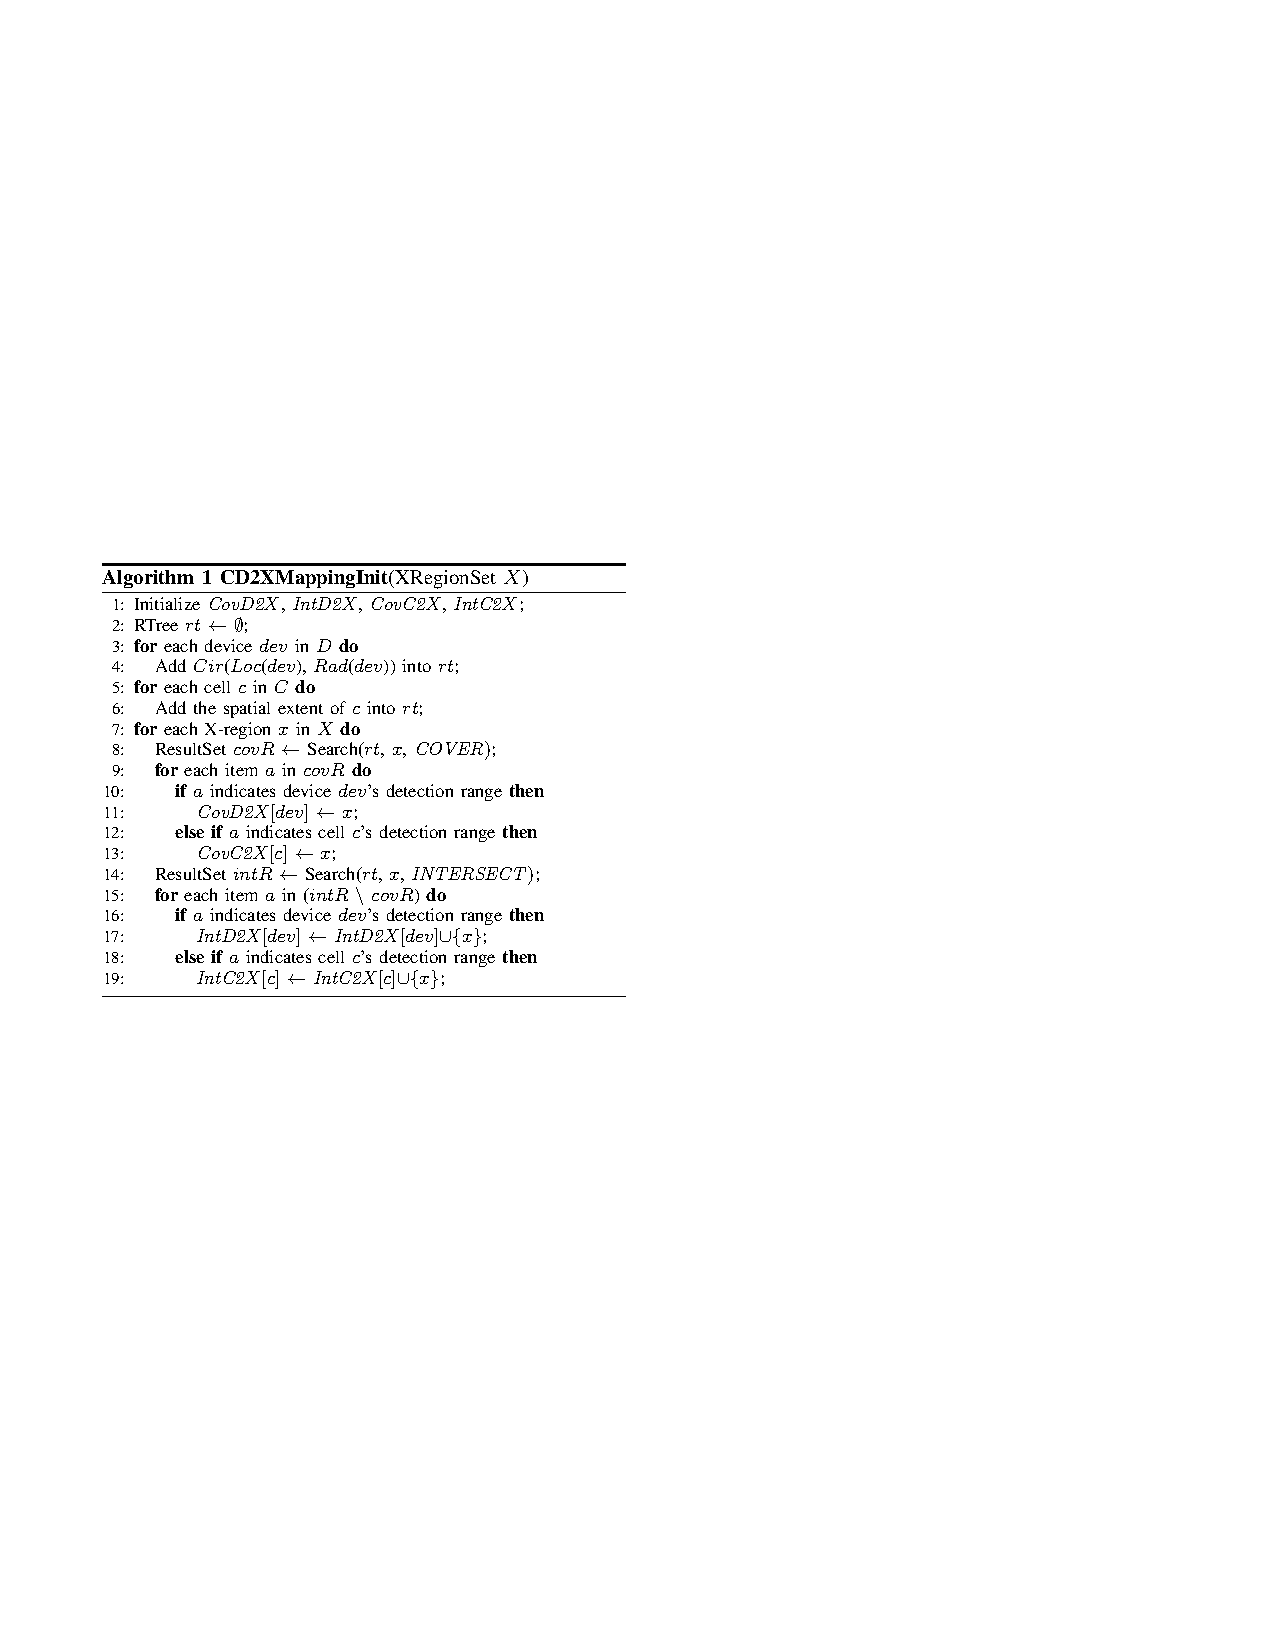
\includegraphics[width=\columnwidth]{figures/2-4/2-4-6.pdf}
  \end{figure}

  \column{0.48\textwidth}
  \begin{sitemize}
    \item $\mn{CovD2X: D \rightarrow IR_X}$ maps a device to an $\mn{X}$-Region that fully covers the device's detection range;
    \item $\mn{IntD2X: D \rightarrow IR_X}$ maps a device to an $\mn{X}$-Region that only intersects the device's detection range;
    \item $\mn{CovC2X: C \rightarrow IR_X}$ maps a cell to an $\mn{X}$-Region that fully covers this cell;
    \item $\mn{IntC2X: C \rightarrow IR_X}$ maps a cell to an $\mn{X}$-Region that only intersects with;
  \end{sitemize}

\end{columns}

\end{frame}

%------------------------------------------------

\begin{frame}
\frametitle{Processing PTISSJ Queries: Partitioning Phase}

\begin{columns}[c]

  \column{.47\textwidth}
  \vspace{-10pt}
  \begin{figure}[tb]
    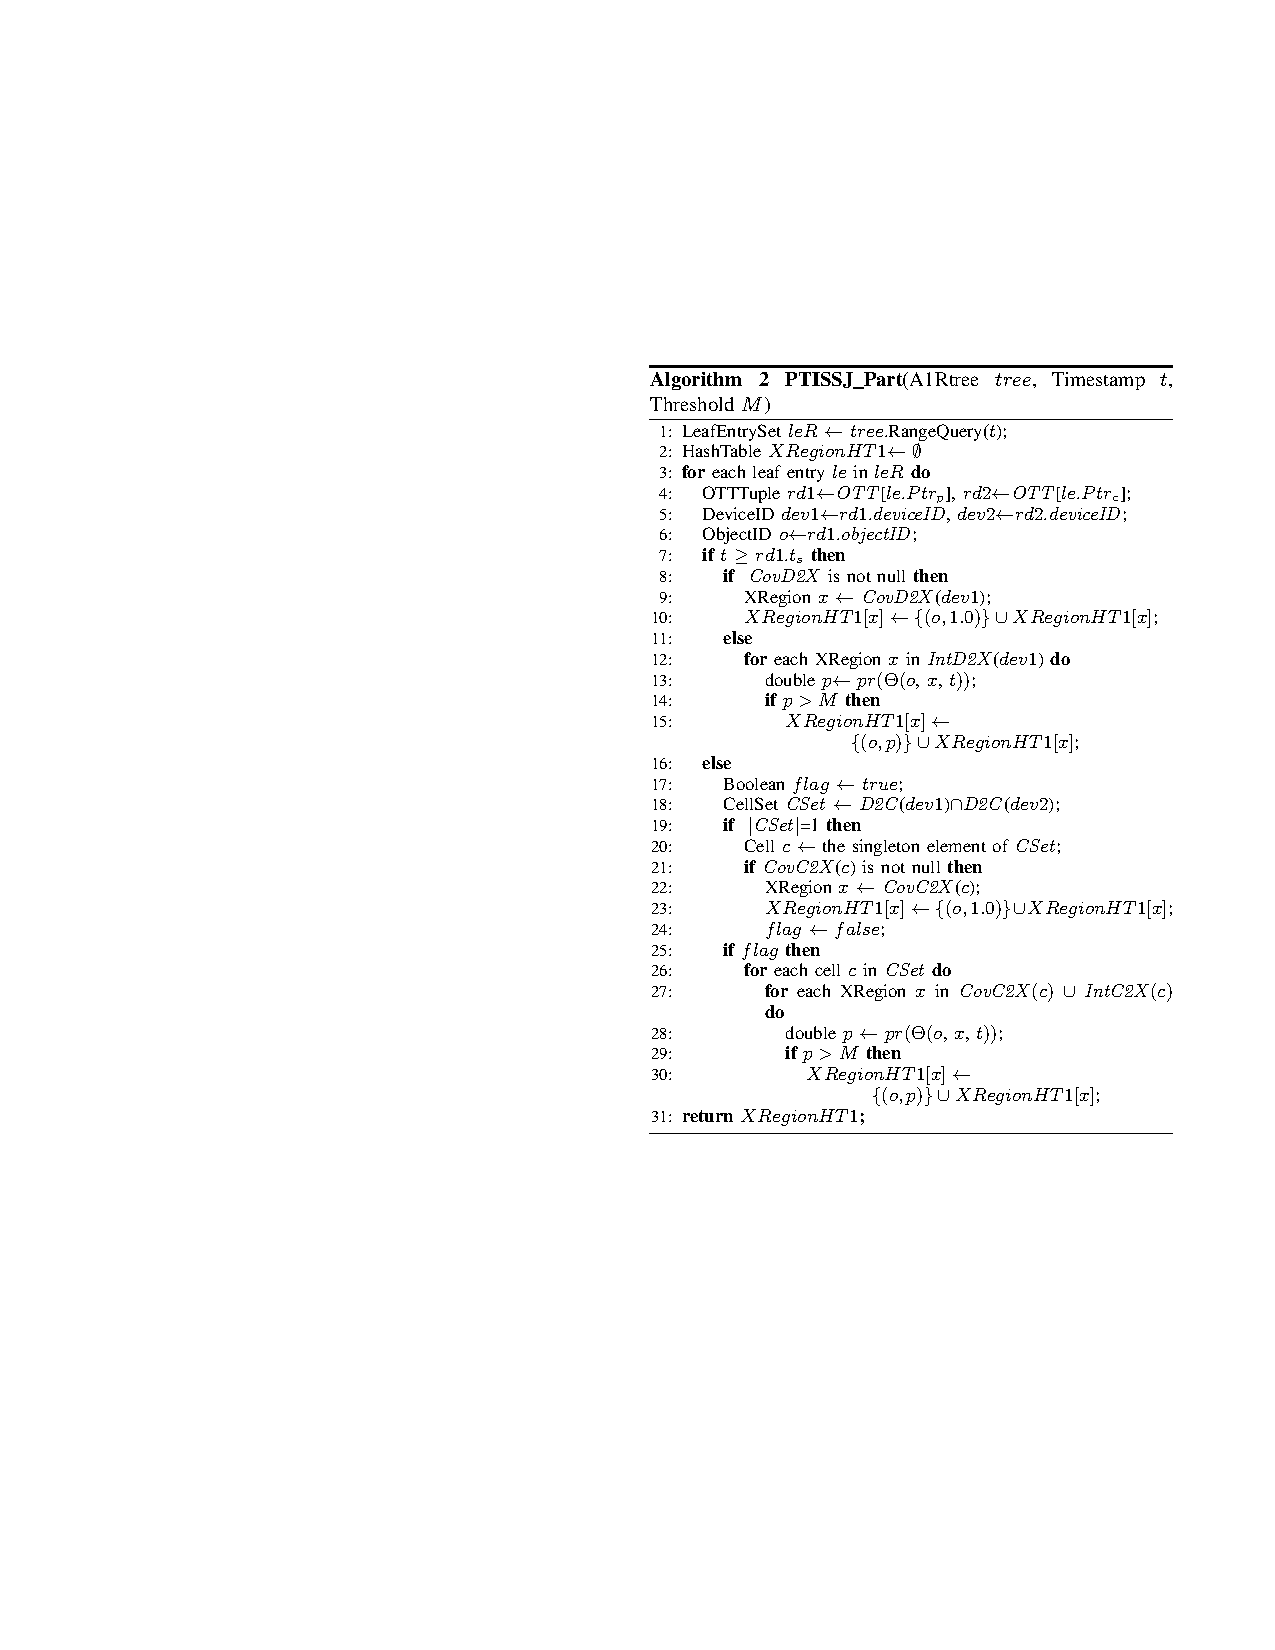
\includegraphics[width=\columnwidth]{figures/2-4/2-4-7.pdf}
  \end{figure}

  \column{0.53\textwidth}
  \begin{fitemize}
    \item all indoor objects are partitioned into buckets that each refers to a distinct $\mn{X}$-region
    \item first, A1R-tree is searched to get all leaf entries whose interval $\mn{(t^{\vdash},t^{\dashv}]}$ contains the join time $\mn{t}$
    \item second, the spatial examination obtains all relevant $\mn{X}$-region in which $\mn{o_i}$ may be at time $\mn{t}$
    \item the relevant probabilities are evaluated for each object, and the necessary records are generated and added to relevant buckets, for each $\mn{p_l = pr(\Theta(o_i, x_l, t))}$, if it is larger than threshold $\mn{M}$, insert the record into buckets.
  \end{fitemize}

\end{columns}

\end{frame}

%------------------------------------------------

\begin{frame}
\frametitle{Processing PTISSJ Queries: Partitioning Phase}

\begin{columns}[c]

  \column{.5\textwidth}
  \textbf{Active State}~\\
  \ssize{
  \textrm{object $\mn{o_i}$ must be in device $\mn{dev}$'s detection range at time $\mn{t}$}.~\\
  \begin{enumerate}
    \item if the detection range is fully covered by an $\mn{X}$-region $\mn{x_l}$, as indicated by $\mn{CovD2X(dev_c) = x_l}$, a record $\mn{(o_i, 1.0)}$ is added to $\mn{x_l}$'s bucket;
    \item otherwise, $\mn{dev_c}$'s detection range intersects with each $\mn{X}$-region in $\mn{CovD2X(dev_c)}$, evaluated the probability, if it is larger than $\mn{M}$, add to the bucket.
  \end{enumerate}
  }

  \column{0.5\textwidth}
  \textbf{Inactive State}~\\
  \ssize{
  \textrm{object $\mn{o_i}$ must be in a cell in $\mn{Cells_{mid} = D2C(dev_p) \cap D2C(dev_c)}$}.~\\
  \begin{enumerate}
    \item if $\mn{Cells_{mid}}$ is the singleton set and the cell is covered by one $\mn{X}$-region $\mn{x_l}$, indicated by $\mn{CovC2X(c)= x_l}$, a record $\mn{(o_i, 1.0)}$ is added to $\mn{x_l}$'s bucket;
    \item otherwise, the single cell $\mn{c}$ in $\mn{Cells_{mid}}$ intersects with several $\mn{X}$-regions (indicated by $\mn{CovC2X(c)}$), or $\mn{Cells_{mid}}$ contains several cells.
  \end{enumerate}
  }

\end{columns}

\end{frame}


\subsection{2.5 A Foundation for Efficient Indoor Distance-aware Query Processing} % A subsection can be created just before a set of slides with a common theme to further break down your presentation into chunks

%\begin{frame}
\frametitle{About This Work...}

\emph{A Foundation for Efficient Indoor Distance-Aware Query Processing}.~\cite{DBLP:conf/icde/LuYCJ11} \\
H.~Lu, X.~Cao, and C.~S. Jensen.\\~\\

\begin{itemize}
  \item Published at \emph{ICDE' 2012}.
  \item First time to propose a distance-aware indoor space model that integrates indoor distance seamlessly.
  \item Accompanying, efficient algorithms for computing indoor distances.
  \item Indexing framework that accommodates indoor distances.
\end{itemize}

\end{frame}

%------------------------------------------------

\begin{frame}
\frametitle{Motivation}

\begin{itemize}
  \item A variety of LBS services are useful in indoor space.
    \begin{fitemize}
      \item a museum guidance service in a complex exhibition
      \item boarding reminder service in an airport, to remind the passengers especially those far away from their gates or departures
    \end{fitemize}

  \item Such indoor LBSs will benefit from the availability of accurate indoor distances.
    \begin{fitemize}
      \item indoor space entities enable as well as constrain indoor movement, thus makes traditional space model for Euclidean/spatial network spaces unsuitable.
      \item existing indoor space models~\cite{becker2005location, li2008lattice, becker2009multilayered} pay little attention to indoor distances.
    \end{fitemize}

\end{itemize}

\end{frame}

%------------------------------------------------

\begin{frame}
\frametitle{Indoor Topology Mapping Structures}

Mapping $D2P$ maps a door $d_k$ to one or two partition pairs~\footnote{\ssize{the basic assumption that a door corresponds to two doors can be extended by converting a door to multiple doors.}} $(v_i, v_j)$ such that one can move from partition~\footnote{\ssize{a partition indicates a room, a hallway or a staircase.}} $v_i$ to partition $v_j$ through door $d_k$:
\pause
\begin{equation}
 D2P: \mathcal{S}_{door} \rightarrow 2^{\mathcal{S}_{partition}} \times 2^{\mathcal{S}_{partition}}
\end{equation}
\pause
For \emph{enterable partition} of door $d_k$:
\pause
\begin{equation}
 D2P_{\sqsupset}: \mathcal{S}_{door} \rightarrow 2^{\mathcal{S}_{partition}}
\end{equation}
\pause
For \emph{leaveable partition} of door $d_k$:
\pause
\begin{equation}
 D2P_{\sqsubset}: \mathcal{S}_{door} \rightarrow 2^{\mathcal{S}_{partition}}
\end{equation}
\end{frame}

%------------------------------------------------

\begin{frame}
\frametitle{Indoor Topology Mapping Structures}


The mapping $P2D_{\sqsupset}$ maps a partition $v$ to all the doors through which one can enter $v$:
\pause
\begin{equation}
 P2D_{\sqsupset}: \mathcal{S}_{partition} \rightarrow 2^{\mathcal{S}_{door}}
\end{equation}
\pause
The mapping $P2D_{\sqsubset}$ maps a partition $v$ to all the doors through which one can leave $v$:
\pause
\begin{equation}
 P2D_{\sqsubset}: \mathcal{S}_{partition} \rightarrow 2^{\mathcal{S}_{door}}
\end{equation}
\pause
The mapping $P2D$ is used when there's no need to differentiate the directionality:
\pause
\begin{equation}
 P2D(v_i): P2D_{\sqsupset}(v_i) \cup P2D_{\sqsubset}(v_i)
\end{equation}
\end{frame}

%------------------------------------------------

\begin{frame}
\frametitle{Accessibility Base Graph}

\begin{columns}[c]

  \column{0.52\textwidth}
  \vspace{-15pt}
  \begin{figure}[tb]
    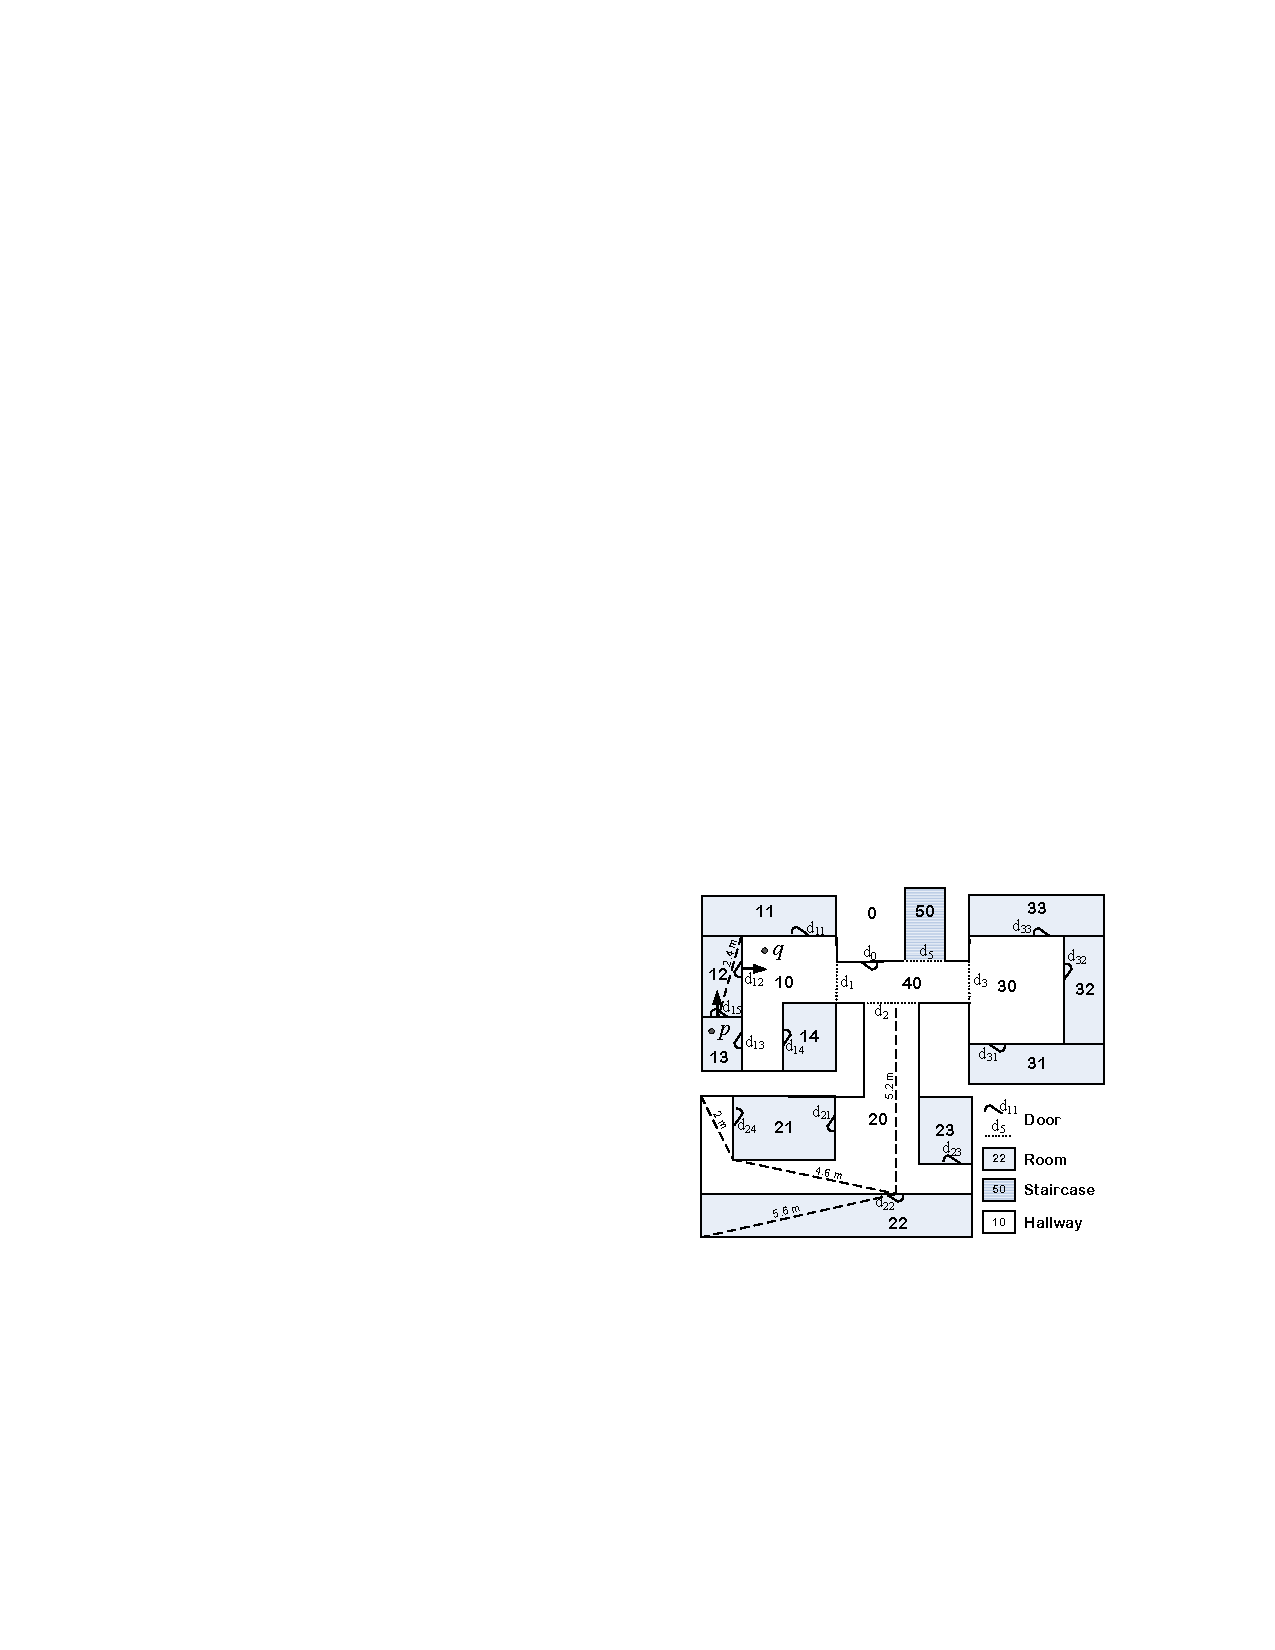
\includegraphics[width=0.85\columnwidth]{figures/2-5/2-5-1.pdf}
  \end{figure}
  \begin{example}
    \textrm{
    \ssize{
      $D2P_{\sqsupset}(d_{12}) = \{ v_{10}\}$, $D2P_{\sqsubset}(d_{12}) = \{ v_{12}\}$
      $P2D_{\sqsupset}(v_{13}) = \{ d_{13}\}$, $P2D_{\sqsubset}(v_{13}) = \{ d_{13}, d_{15}\}$
    }
    }
  \end{example}

  \column{0.48\textwidth}
  \vspace{-15pt}
  \begin{figure}[tb]
    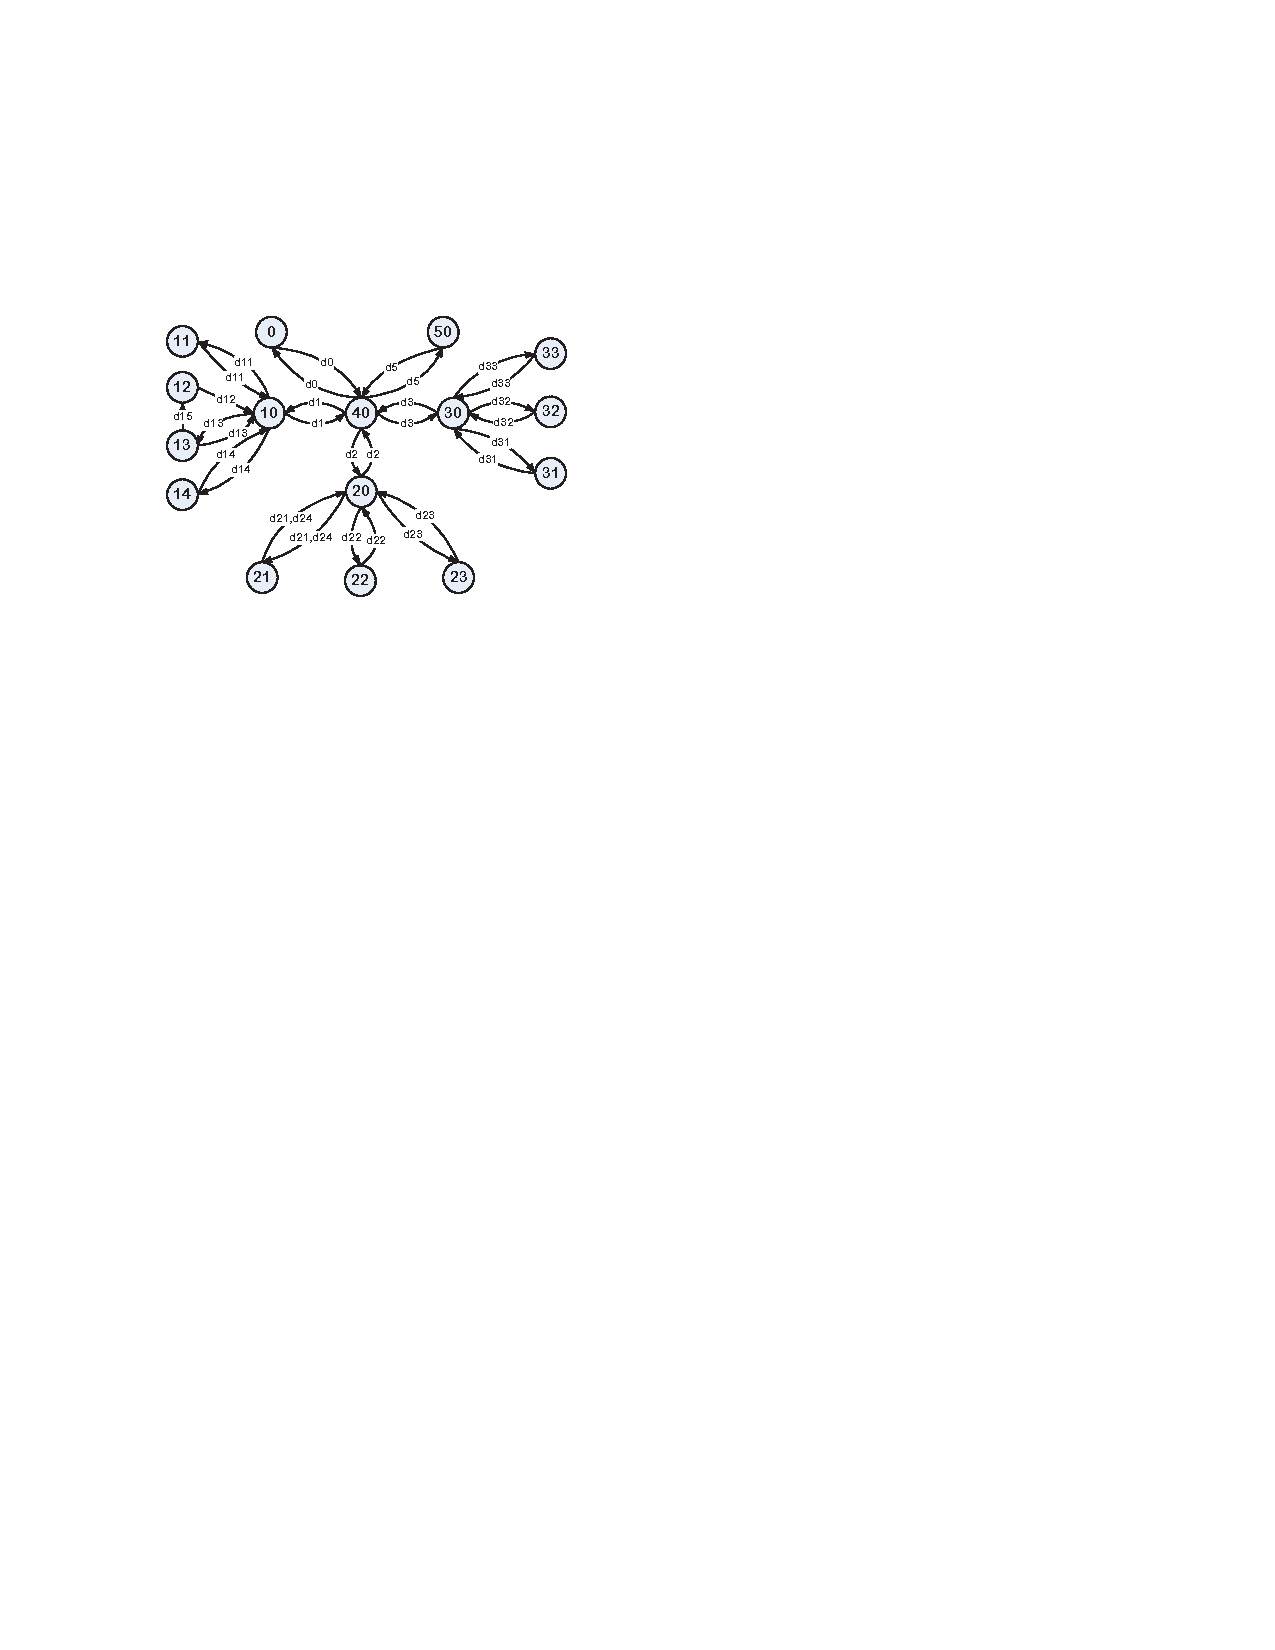
\includegraphics[width=0.8\columnwidth]{figures/2-5/2-5-2.pdf}
  \end{figure}
  \vspace{-10pt}
  \begin{block}{Accessibility Base Graph}
    \textrm{
    \ssize{
    \begin{itemize}
      \item $G_{accs} = \{V, E_a, L\}$
      \item $V = \mathcal{S}_{partition}$ is the set of vertices
      \item $E_a = \{ (v_i, v_j, d_k) | (v_i, v_j) \in D2P(d_k) \}$ is the set of labeled, directed edges
      \item $L = \mathcal{S}_{door}$ is the set of edge labels
    \end{itemize}
    }
    }
  \end{block}

\end{columns}

\end{frame}

%------------------------------------------------

\begin{frame}
\frametitle{Distance-Aware Model}

\fsize{\textrm{The $G_{accs}$ graph does not capture indoor distance information. \conceptbf{Extended Graph Model} is proposed to integrate indoor distances into the graph in a seamless way. \emph{Minimum Indoor Walking Distance}(MIWD) is used. }}

\begin{block}{Extended Graph Model $G_{dist} = \{ V, E_a, L, f_{dv}, f_{d2d} \}$}
  \textrm{
  \begin{sitemize}
    \item $V = \mathcal{S}_{partition}$ is the set of vertices
    \item $E_a = G_{accs}.E_a$
    \item $L = \mathcal{S}_{door}$ is the set of edge labels
    \item $f_{dv} = \mathcal{S} \times V \rightarrow \mathcal{R} \cup \{ \infty \}$ maps an edge to a distance value.
    \begin{equation*}
      f_{dv} = \left\{\begin{matrix}
                \max_{p \in v_j}|| d_i, p || , & if~~ v_j \in D2P_{\sqsupset};
                \\
                \infty , & otherwise.
                \end{matrix}\right.
    \end{equation*}
    \item $f_{d2d} = V \times \mathcal{S}_{door} \times \mathcal{S}_{door} \rightarrow \mathcal{R} \cup \{ \infty \}$ maps a 3-tuple to a distance value.
    \begin{equation*}
      f_{dv} = \left\{\begin{matrix}
                || d_i, d_j ||_{v_k} , & if~~ d_i \in P2D_{\sqsupset}(v_k) and d_j \in P2D_{\sqsubset}(v_k);
                \\
                \infty , & if~~ d_i = d_j and d_i,d_j \in P2D(v_k);
                \\
                0 , & otherwise.
                \end{matrix}\right.
    \end{equation*}
  \end{sitemize}
  }
\end{block}

\end{frame}

%------------------------------------------------

\begin{frame}
\frametitle{Indoor Distance Computation: \emph{door-to-door distance}}

\begin{columns}[c]

  \column{0.52\textwidth}
  \begin{figure}[tb]
    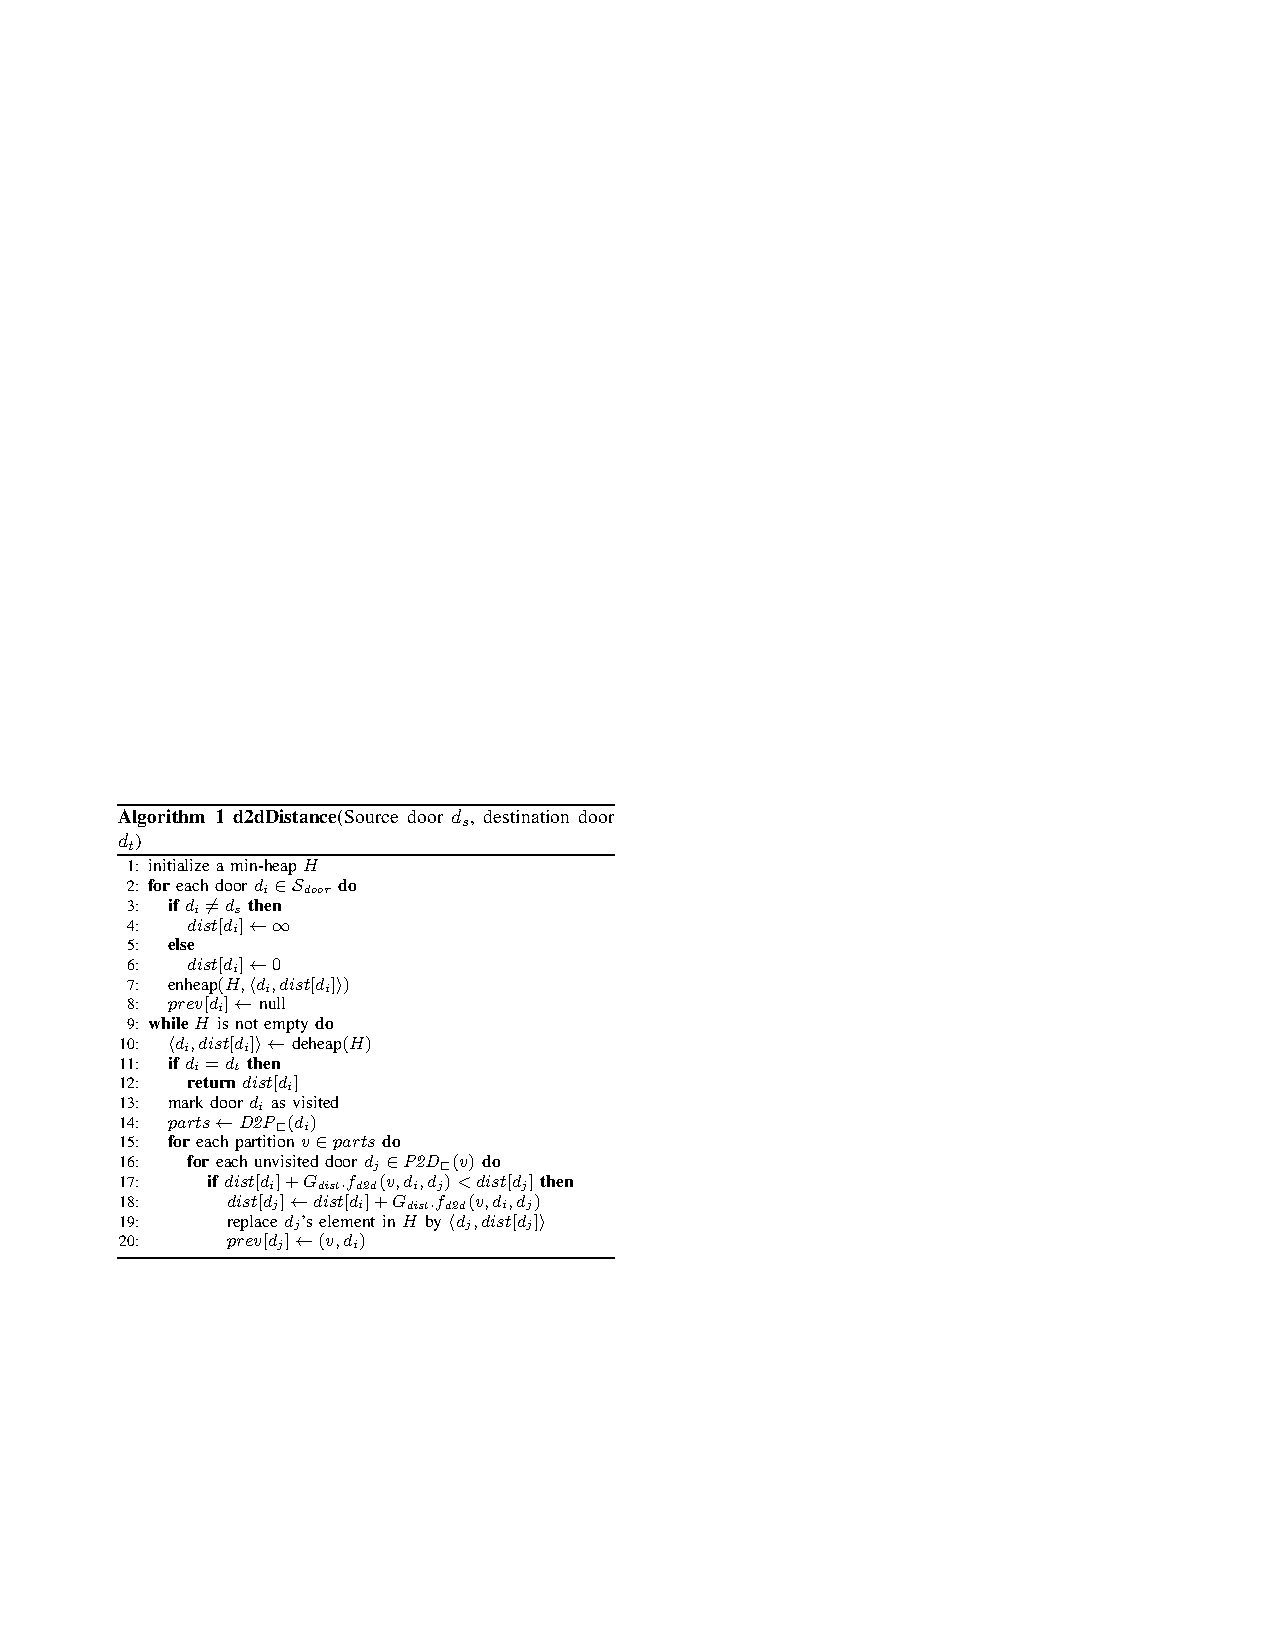
\includegraphics[width=\columnwidth]{figures/2-5/2-5-3.pdf}
  \end{figure}

  \column{0.48\textwidth}


\end{columns}

\end{frame}

%------------------------------------------------

\begin{frame}
\frametitle{Indoor Distance Computation: \emph{point-to-point distance}}

\begin{columns}[c]

  \column{0.52\textwidth}
  \begin{figure}[tb]
    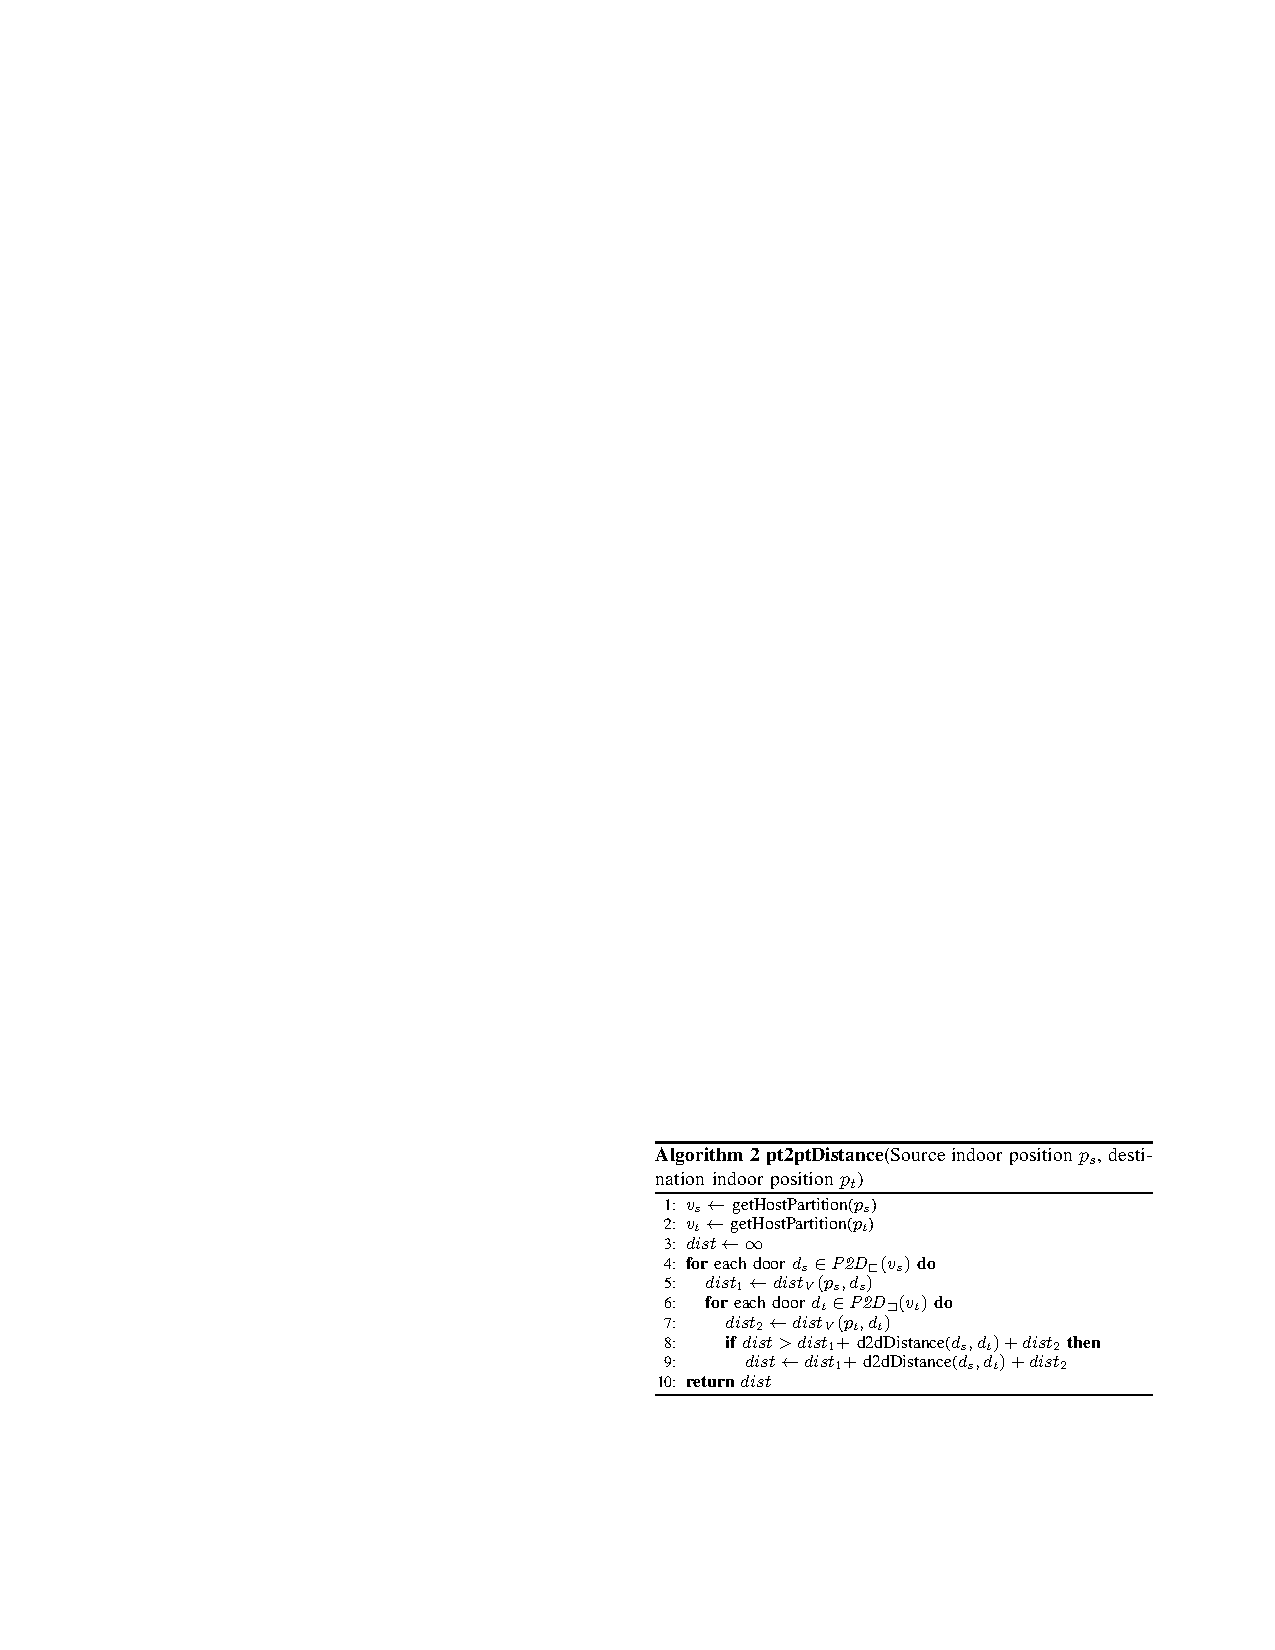
\includegraphics[width=\columnwidth]{figures/2-5/2-5-4.pdf}
  \end{figure}

  \column{0.48\textwidth}


\end{columns}

\end{frame}

%------------------------------------------------

\begin{frame}
\frametitle{Indoor Distance Computation: \emph{point-to-point distance} (I)}

\begin{columns}[c]

  \column{0.52\textwidth}
  \begin{figure}[tb]
    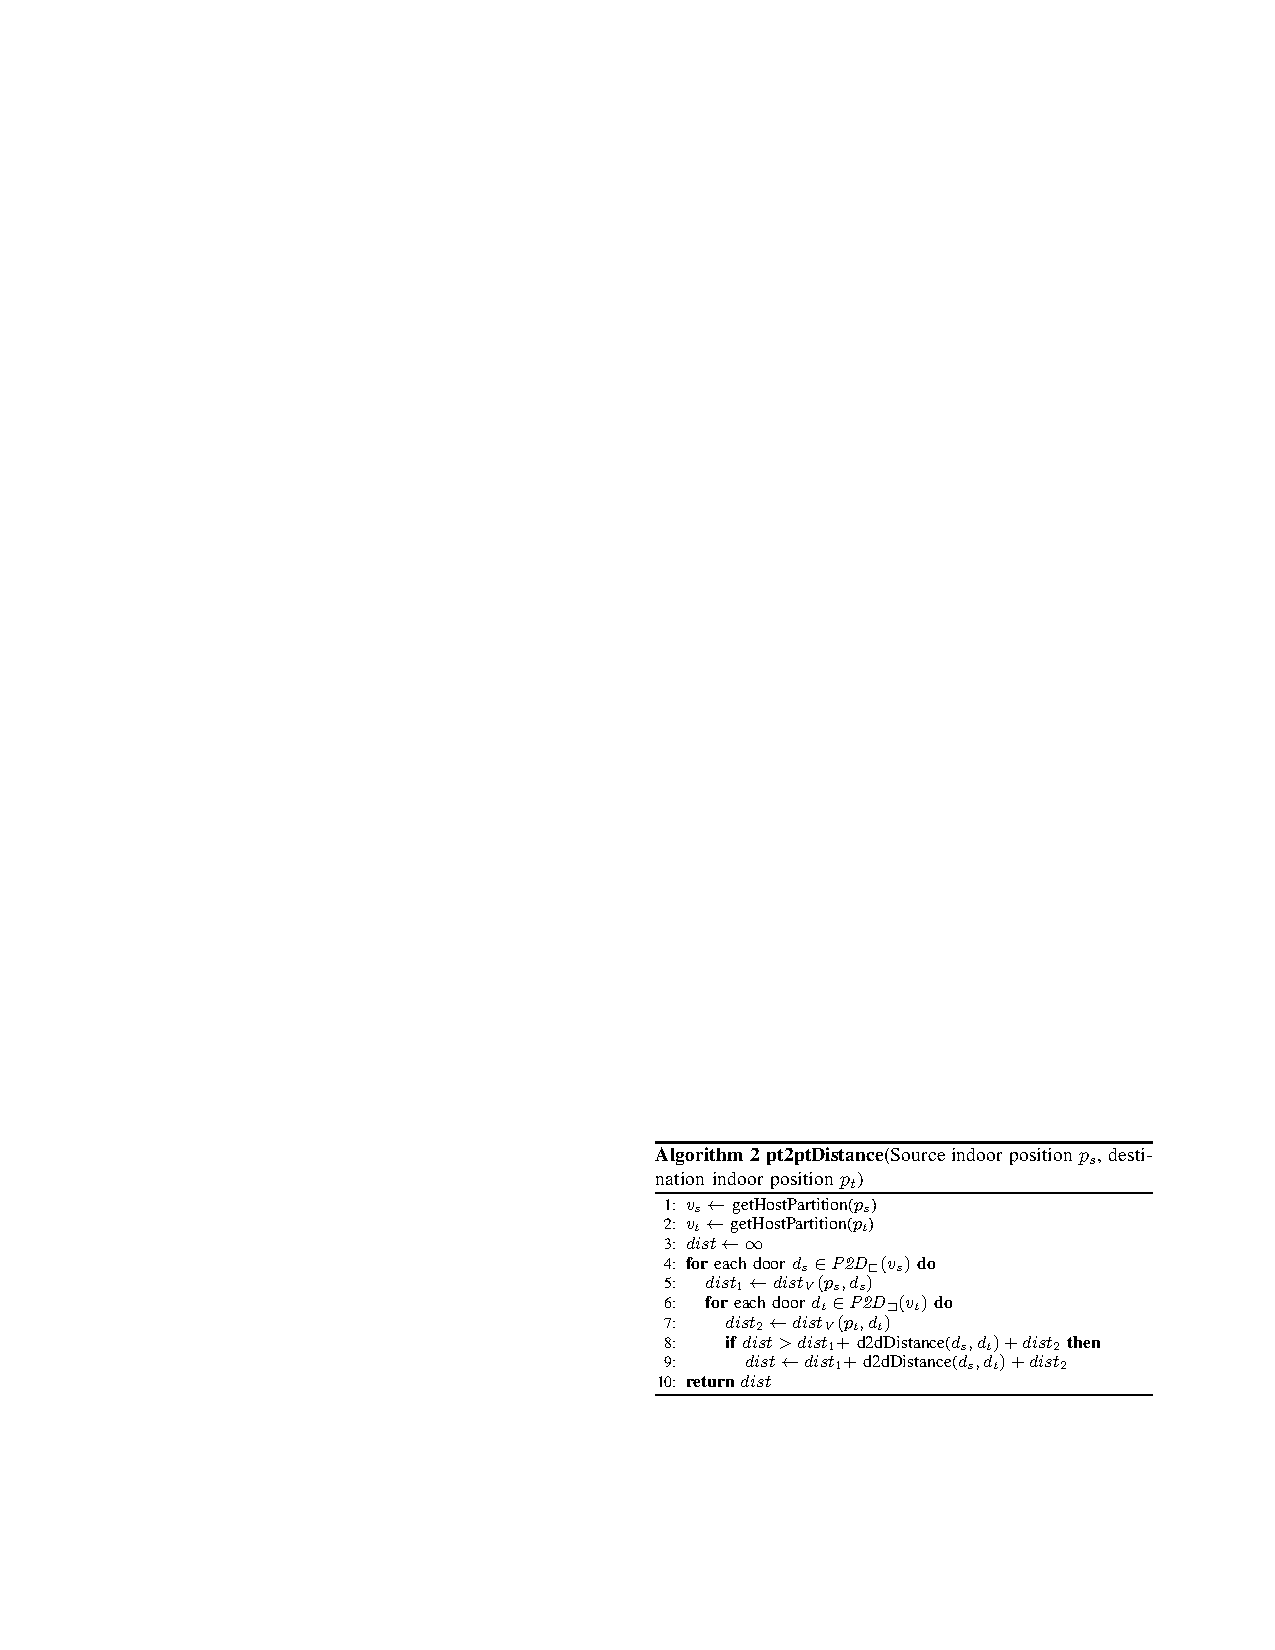
\includegraphics[width=\columnwidth]{figures/2-5/2-5-4.pdf}
  \end{figure}

  \column{0.48\textwidth}


\end{columns}

\end{frame}

%------------------------------------------------

\begin{frame}
\frametitle{Indoor Distance Computation: \emph{point-to-point distance} (II)}

\begin{columns}[c]

  \column{0.4\textwidth}
  \begin{figure}[tb]
    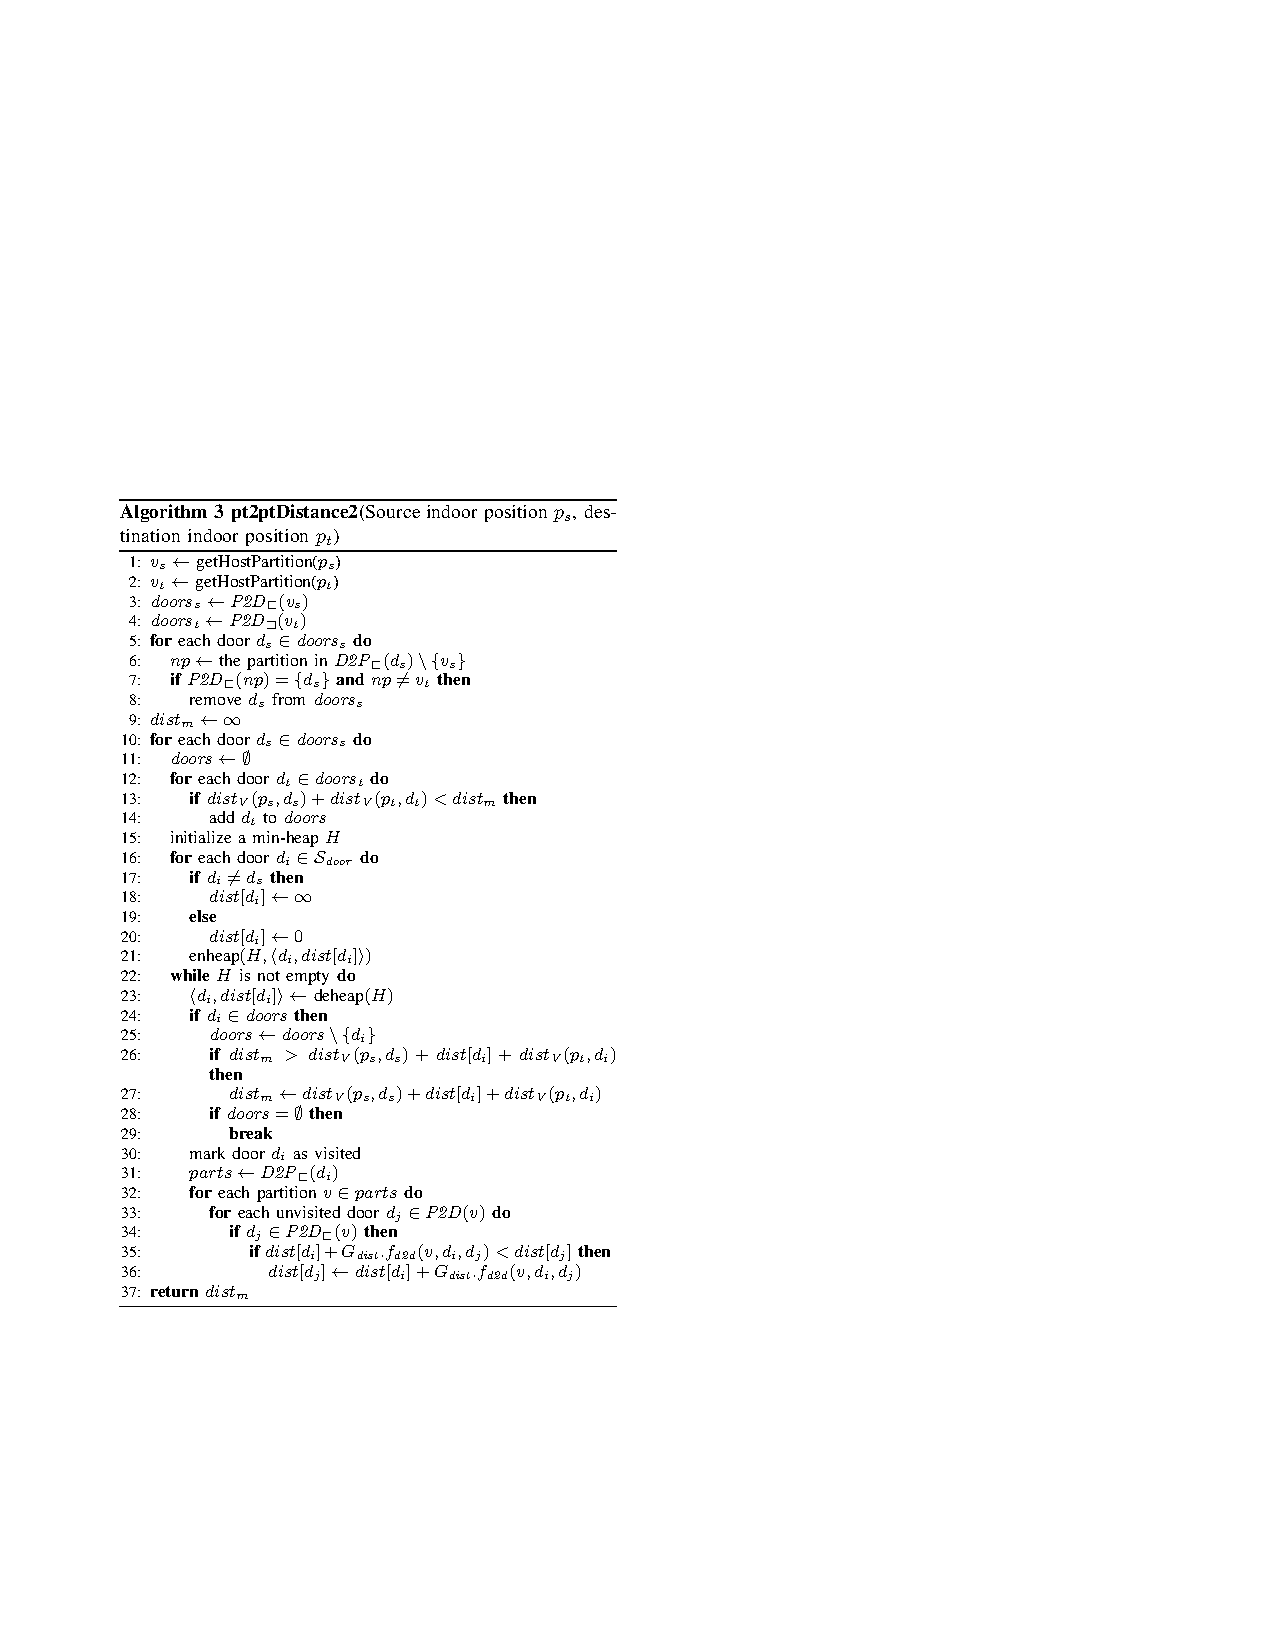
\includegraphics[width=\columnwidth]{figures/2-5/2-5-5.pdf}
  \end{figure}

  \column{0.48\textwidth}


\end{columns}

\end{frame}


% %------------------------------------------------
%
% \begin{frame}
% \frametitle{Indoor Distance Computation: \emph{point-to-point distance} (III)}
%
% \begin{columns}[c]
%
%   \column{0.52\textwidth}
%   \begin{figure}[tb]
%     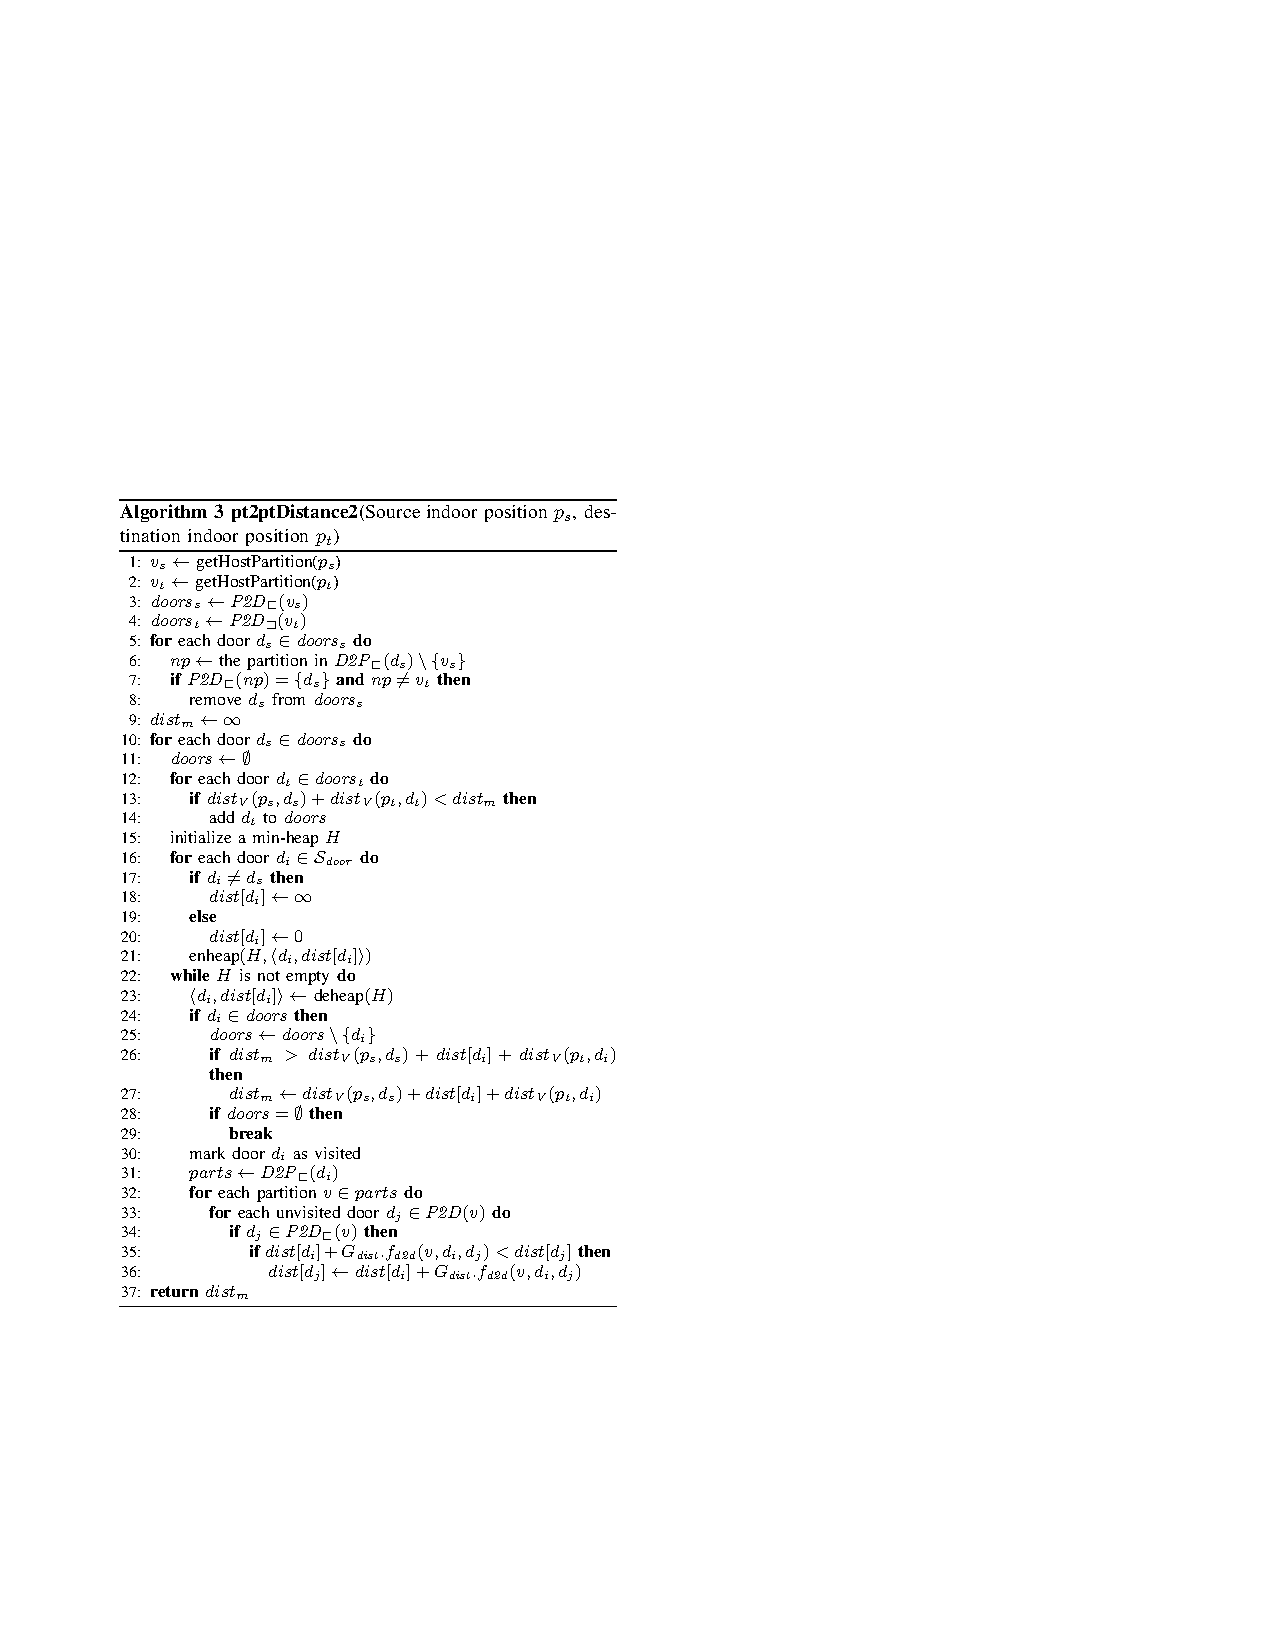
\includegraphics[width=\columnwidth]{figures/2-5/2-5-5.pdf}
%   \end{figure}
%
%   \column{0.48\textwidth}
%
%
% \end{columns}
%
% \end{frame}


\subsection{2.6 Efficient Distance-aware Query Evaluation on Indoor Moving Objects} % A subsection can be created just before a set of slides with a common theme to further break down your presentation into chunks

%\begin{frame}
\frametitle{About This Work...}

\emph{Efficient Distance-Aware Query Evaluation on Indoor Moving Objects}.~\cite{DBLP:conf/icde/XieLP13} \\
X.~Xie, H.~Lu, and T.~B. Pedersen.\\~\\

\begin{itemize}
  \item Published at \emph{ICDE' 2013}.
  \item Study indoor distances and effective prunning bounds in relation to indoor moving objects.
  \item Design a composite index for indoor spaces and moving objects.
  \item Define and evaluate range queries as well as $k$nn queries on indoor moving objects.
\end{itemize}

\end{frame}

%------------------------------------------------

\begin{frame}
\frametitle{Motivation}

\begin{itemize}
  \item In many indoor LBS scenarios, appropriate handling of indoor distances and relevant queries is of critical.
    \begin{fitemize}
      \item a cafe in a mall may send message to nearby shoppers to boost its business
      \item in a large airport, it important to minitor individuals within a pre-defined range from a sensitive point
    \end{fitemize}

  \item Indoor spaces are characterized by many special entities and thus render distance calculation very complex.

  \item The limitations of indoor positioning technologies create inherent uncertainties in indoor moving objects data.

\end{itemize}

\end{frame}

%------------------------------------------------

\begin{frame}
\frametitle{Notations}

\begin{figure}[tb]
  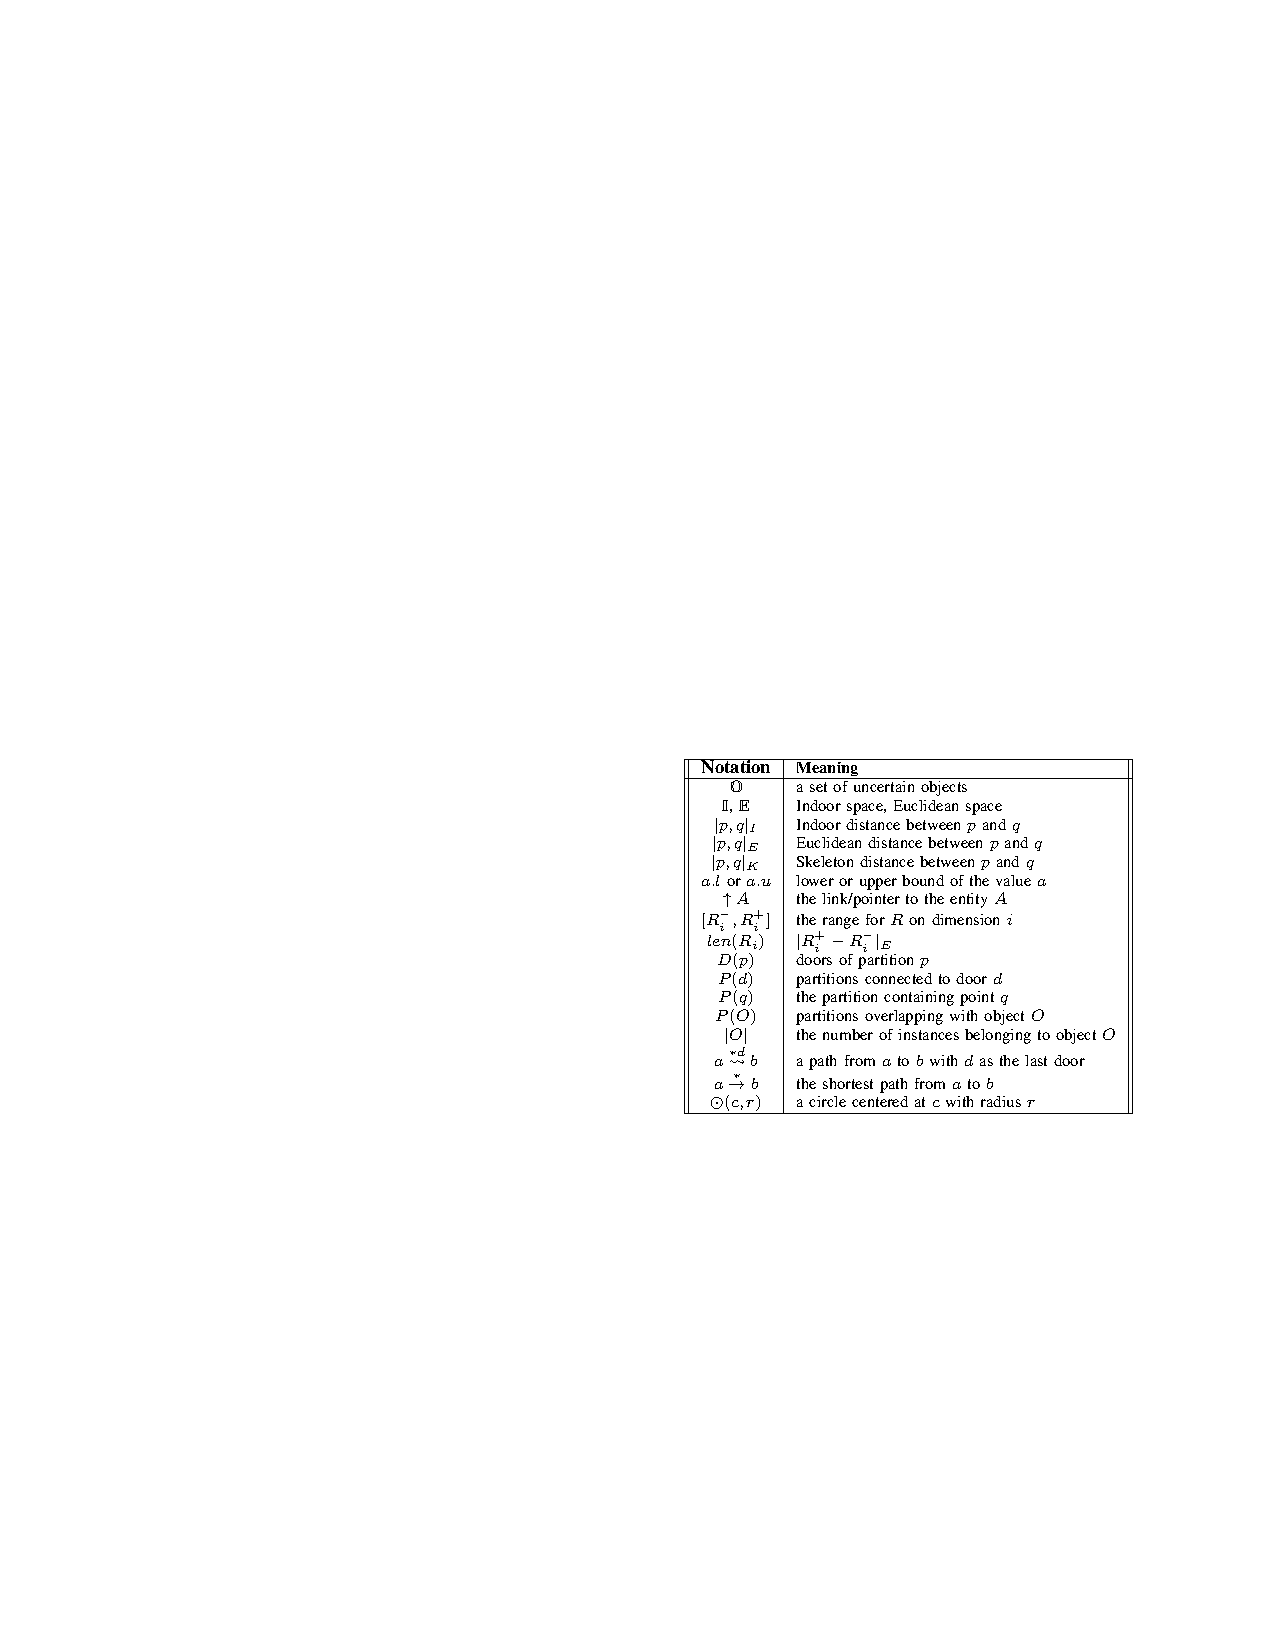
\includegraphics[width=0.75\columnwidth]{figures/2-6/2-6-1.pdf}
\end{figure}

\end{frame}

%------------------------------------------------

\begin{frame}
\frametitle{Preliminaries: Indoor Space and Indoor Distance}

\conceptbf{Doors Graph} has been proposed to represent the connectivity of indoor partitions as well as door-to-door distances.~\cite{DBLP:conf/edbt/YangLJ10}\\~\\\pause

Given two indoor positions $p$ an $q$, we use $q \overset{\delta}{\rightsquigarrow} p$ to denote a path from $q$ to $p$ where $\delta$ is the sequence of doors on the path.\\~\\\pause

The length of the shortest path as \emph{indoor distance} from $q$ to $p$, and denote it formally as $|q, p|_{I} = min_{\delta}(|q \overset{\delta}{\rightsquigarrow} p|)$, also $q \overset{\delta}{\rightarrow} p$.\\~\\\pause

\emph{indoor distance} consists of \emph{door-door distance} and \emph{intra-partition object-door distance}:\pause
\begin{equation}
  min_{d_q \in D(q), d_p \in D(p)}(|q, d_q|_{E} + |d_q, d_p|_{I} + |d_p, p|_{E})
\end{equation}

\end{frame}

%------------------------------------------------

\begin{frame}
\frametitle{Indoor Moving Objects}

\begin{itemize}
  \item Existing proposals~\cite{pfoser1999capturing, DBLP:conf/edbt/YangLJ10} model a moving object by an \emph{uncertainty region}, where the exact location is considered as a random variable inside.
  \item The possibility of its appearance can be collected by object's velocities~\cite{DBLP:conf/edbt/YangLJ10}, parameters of positioning device~\cite{pfoser1999capturing}, or analysis of historical records (represented by \emph{pdf}).
  \item The \emph{pdf} can be either a close form equation~\cite{cheng2003evaluating,cheng2004querying} or a set of instance representation~\cite{kriegel2007probabilistic}, as it is general for arbitrary distribution.
  \item Thus, an indoor moving object $O$ is represented by a set ${(s_i, p_i)}$, where $s_i$ is an instance and $p_i$ is its \emph{existential probability}, satisfying $\sum_{s_i \in O}p_i = 1$.
\end{itemize}

\end{frame}

%------------------------------------------------

\begin{frame}
\frametitle{Expected Indoor Distance}

\begin{definition}[Expected Indoor Distance for Uncertain Object]
  Given a fixed point $q \in \mathbb{I}$ and an uncertain object $O$, the indoor distance from $q$ to $O$ is
  \begin{equation}
    |q, O|_{I} = E_{s_i \in O}(|q,s_i|_{I}) = \sum_{s_i \in O}|q,s_i|_{I} \cdot p_i
  \end{equation}
\end{definition}
\vspace{10pt}
an object $O$'s uncertainty region may overlap with multiple partitions. Accordingly, all the instances in $O$ are divided into subsets, i.e., $O = \cup_{1 \leq j \leq m}S[j](1 \leq m \leq |O|)$ where each $S[j]$ corresponds to a different partition, it is called $O$'s \emph{uncertainty subregion}.

\end{frame}

%------------------------------------------------

\begin{frame}
\frametitle{Case of Indoor Distance $|q, O|_I$ (I)}

\conceptbf{Single-Partition Single-Path Distance}~$O$'s uncertainty region falls into one single partition $P$. For an arbitrary $s_i \in O$, the shortest path $q \overset{*d}{\rightarrow} s_i$ shares the path enters $P$ to reach $s_i$.

\begin{equation}
  |q, O|_{I} = |q,d|_I + \sum_{s_i \in O}|d, s_i|_E \cdot p_i
\end{equation}

\end{frame}

%------------------------------------------------

\begin{frame}
\frametitle{Case of Indoor Distance $|q, O|_I$ (II)}

\conceptbf{Single-Partition Multi-Path Distance}~$O$'s uncertainty region still falls into one single partition $P$. However, for different instances $s_i$ and $s_j$, the shortest path $q \overset{*}{\rightarrow} s_i$ and $q \overset{*}{\rightarrow} s_j$ do not share the same door sequence.

\begin{equation}
  |q, O|_{I} = \sum_{s_i \in O}|q, s_i|_I \cdot p_i
\end{equation}

\begin{columns}[c]

  \column{0.24\textwidth}
  \begin{figure}[tb]
    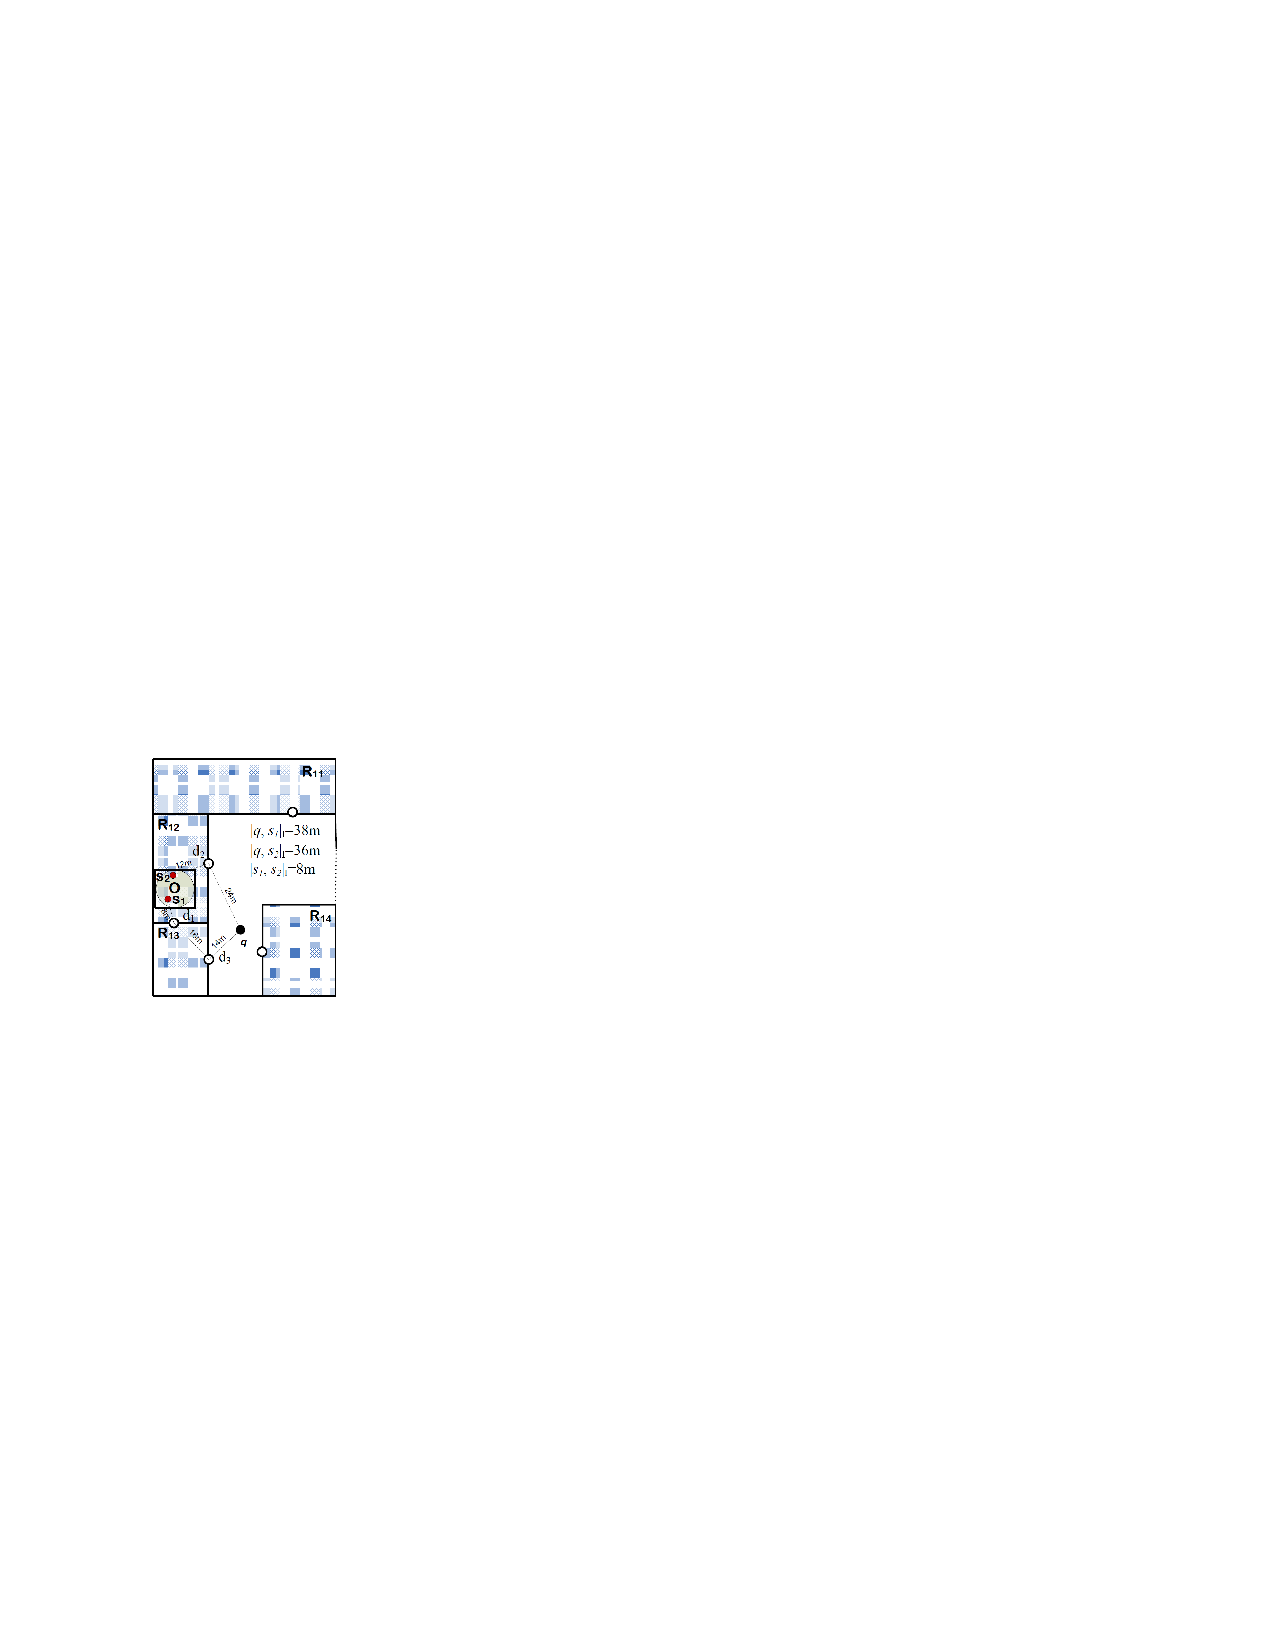
\includegraphics[width=\columnwidth]{figures/2-6/2-6-2.pdf}
  \end{figure}

  \column{0.76\textwidth}
  \begin{example}
    $O$ has two instance $s_1$ and $s_2$, the shortest path from $q$ to them are: $q \overset{d_3, d_1}{\rightsquigarrow} s_1$ and $q \overset{d_2}{\rightsquigarrow} s_2$.
  \end{example}

\end{columns}

\end{frame}

%------------------------------------------------

\begin{frame}
\frametitle{Case of Indoor Distance $|q, O|_I$ (II)}

The \emph{solution space} of the single-partition multi-path distance is the \conceptbf{Additive Weighted Voronoi Diagram}.\\~\\

Suppose partition $P$ has doors $\{d_1, ..., d_m\}$, for each door $d_i$, a weight $w_i = |q, d_i|_I$ is assigned. Use \emph{weighted bisectors} to represent the \emph{Additive Weighted Voronoi Diagram}. Given two doors $d_i$ and $d_j$, whose weights are $w_i$ and $w_j$, respectively, the \emph{weighted bisector} $b_{ij}$ is a curve:
\begin{equation}
  b_{ij} = \{ p : |p,d_i|_E + w_i = |p,d_j|_E + w_j \}
\end{equation}

\vspace{-20pt}
\begin{columns}[c]

  \column{0.2\textwidth}
  \begin{figure}[tb]
    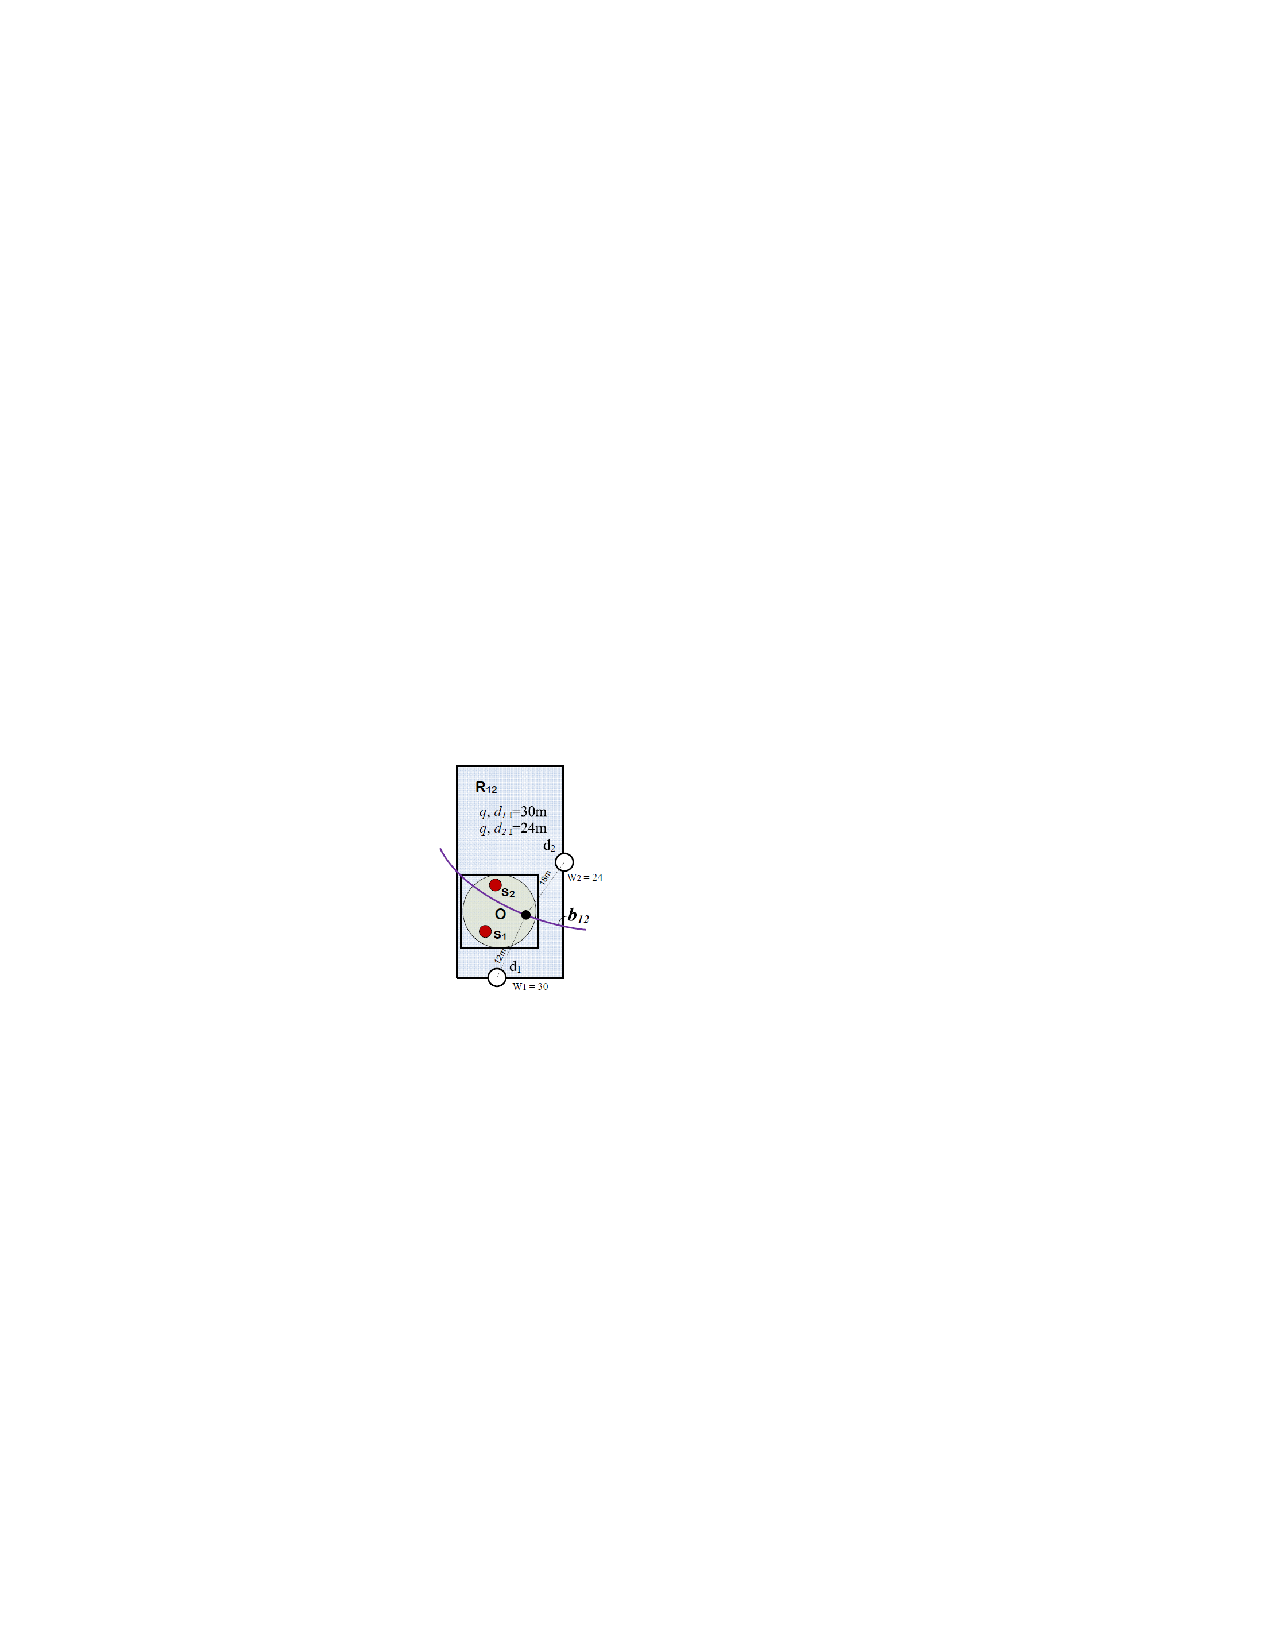
\includegraphics[width=\columnwidth]{figures/2-6/2-6-4.pdf}
  \end{figure}

  \column{0.8\textwidth}
  \begin{figure}[tb]
    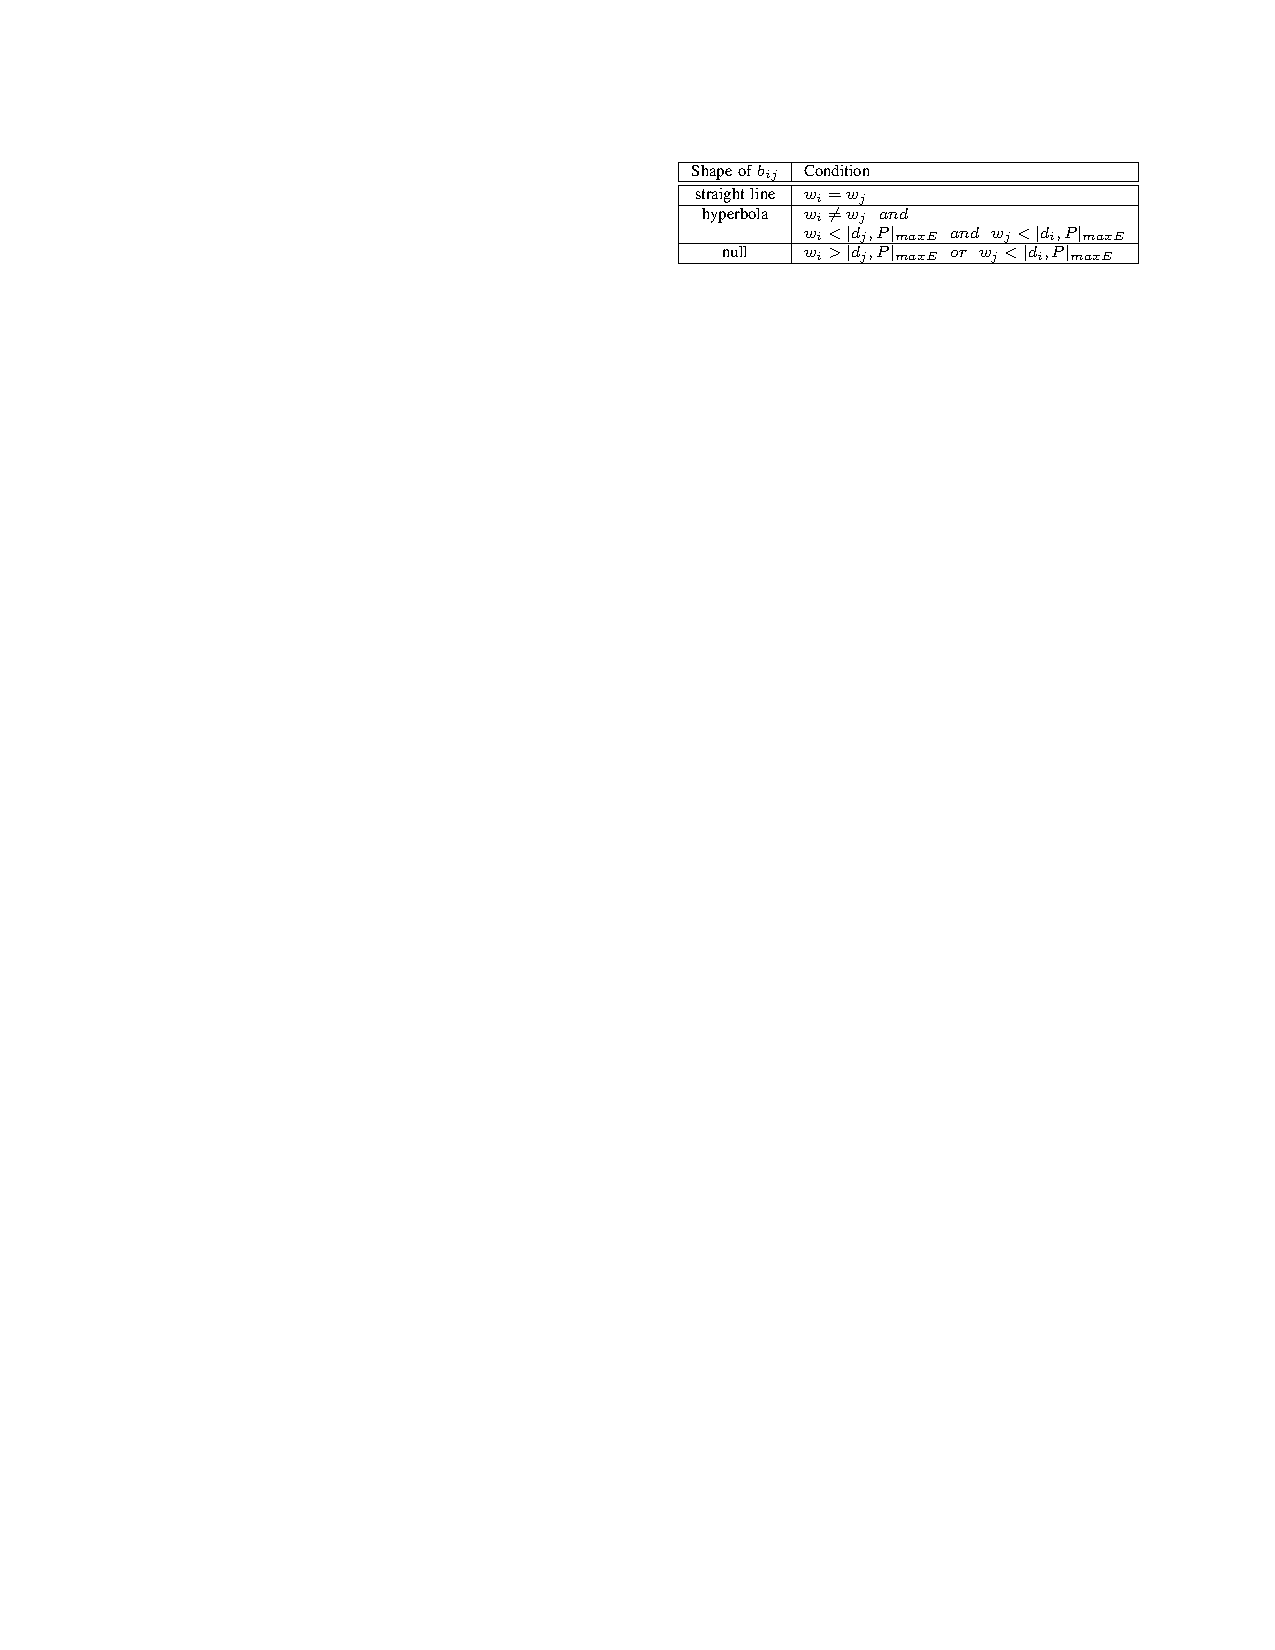
\includegraphics[width=\columnwidth]{figures/2-6/2-6-3.pdf}
  \end{figure}

\end{columns}

\end{frame}

%------------------------------------------------

\begin{frame}
\frametitle{Case of Indoor Distance $|q, O|_I$ (III)}

\conceptbf{Multi-Partition Multi-Path Distance}~$O$'s uncertainty region overlaps with more than one partition, and thus $O = \cup_{1 \leq j \leq m}S[j](1 \leq m \leq |O|)$.

\begin{equation}
  |q, O|_I = \sum_{1 \leq j \leq m}(|q,S[j]|_I \cdot \sum_{s_i \in S[j]}p_i)
\end{equation}

$|q,S[j]|_I$ is calculated according to case I or case II, by substituting $S[j]$ for $O$.

\vspace{-5pt}
\begin{columns}[c]

  \column{0.2\textwidth}
  \begin{figure}[tb]
    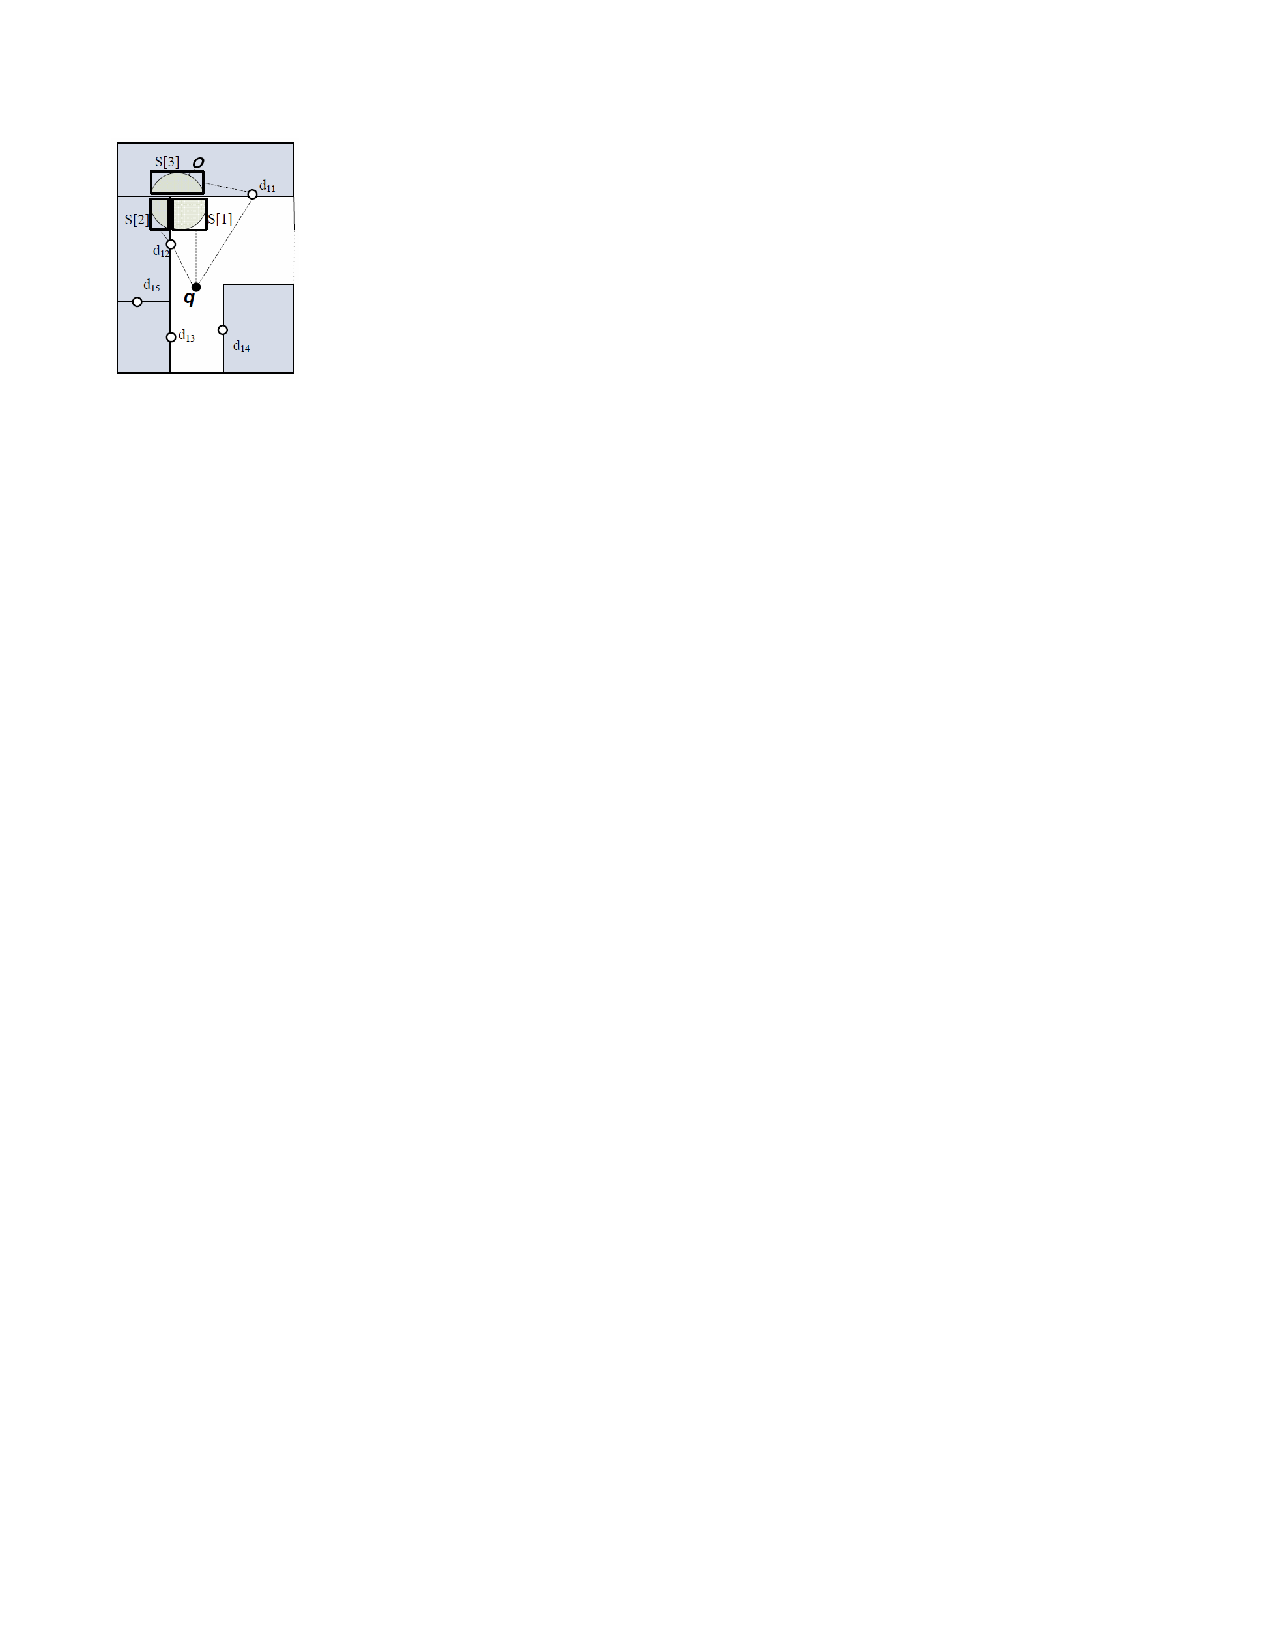
\includegraphics[width=\columnwidth]{figures/2-6/2-6-5.pdf}
  \end{figure}

  \column{0.8\textwidth}
  \begin{example}
    $O$ has three uncertainty subregions $S_1$, $S_2$ and $S_3$. Accordingly, $|q,O|_I = E(\sum_{1 \leq j \leq 3}(|q, S[j]_I|))$.
  \end{example}

\end{columns}

\end{frame}

%------------------------------------------------

\begin{frame}
\frametitle{Bounds for Indoor Distances}

\conceptbf{Euclidean Lower Bounds}

\vspace{10pt}
\begin{lemma}[Euclidean Lower Bounds]
  For point $q$ and object $O$ in an indoor space, the (virtual) Euclidean distance between them is the lower bound of their indoor space. Therefore, it has $|q,O|_{minE} \leq |q,O|_I$, where $|q, O|_{minE} = \min_{s_i \in O}|q,s_i|_E$.
\end{lemma}

\vspace{10pt}
\textrm{it is impossible to derive the indoor upper bounds by using Euclidean distances only.}

\end{frame}

%------------------------------------------------

\begin{frame}[allowframebreaks]
\frametitle{Bounds for Indoor Distances}

\conceptbf{Indoor Toplogical ULBounds}

\begin{lemma}[Toplogical Lower Bounds]
  \ssize{
  Let $t_{min}(S[i])$ be: $$\min_{d_q \in D(P(q)), d_s \in D(P(S[i]))}|q,d_q|_E + |d_q \overset{*}{\rightarrow} d_s| + |d_s, S[i]|_{minE}$$. Then, $|q,O|_I \geq min\{ t_{min}(S[i]) \}$.
  }
\end{lemma}

\begin{lemma}[Toplogical Upper Bounds]
  \ssize{
  Let $t_{max}(S[i])$ be: $$\min_{d_q \in D(P(q)), d_s \in D(P(S[i]))}|q,d_q|_E + |d_q \overset{*}{\rightarrow} d_s| + |d_s, S[i]|_{maxE}$$. Then, $|q,O|_I \leq max\{ t_{max}(S[i]) \}$.
  }
\end{lemma}

\textrm{a looser topological upper bound is more economic to be derived, it also requires knowing some paths connecting point $q$ and subregion $S[i]$}:

\begin{lemma}[Toplogical Looser Upper Bounds, TLU]
  \ssize{
  Let $t_{max}(S[i])$ be: $$\min_{d_q \in D(P(q)), d_s \in D(P(S[i]))}|q,d_q|_E + |d_q \overset{*}{\rightsquigarrow} d_s| + |d_s, S[i]|_{maxE}$$. Then, $|q,O|_I \leq max\{ t_{max}(S[i]) \}$.
  }
\end{lemma}

\end{frame}

%------------------------------------------------

\begin{frame}
\frametitle{Bounds for Indoor Distances}

\conceptbf{Indoor Probabilistic ULBounds}

\vspace{10pt}
\begin{columns}[c]

  \column{0.3\textwidth}
  \begin{figure}[tb]
    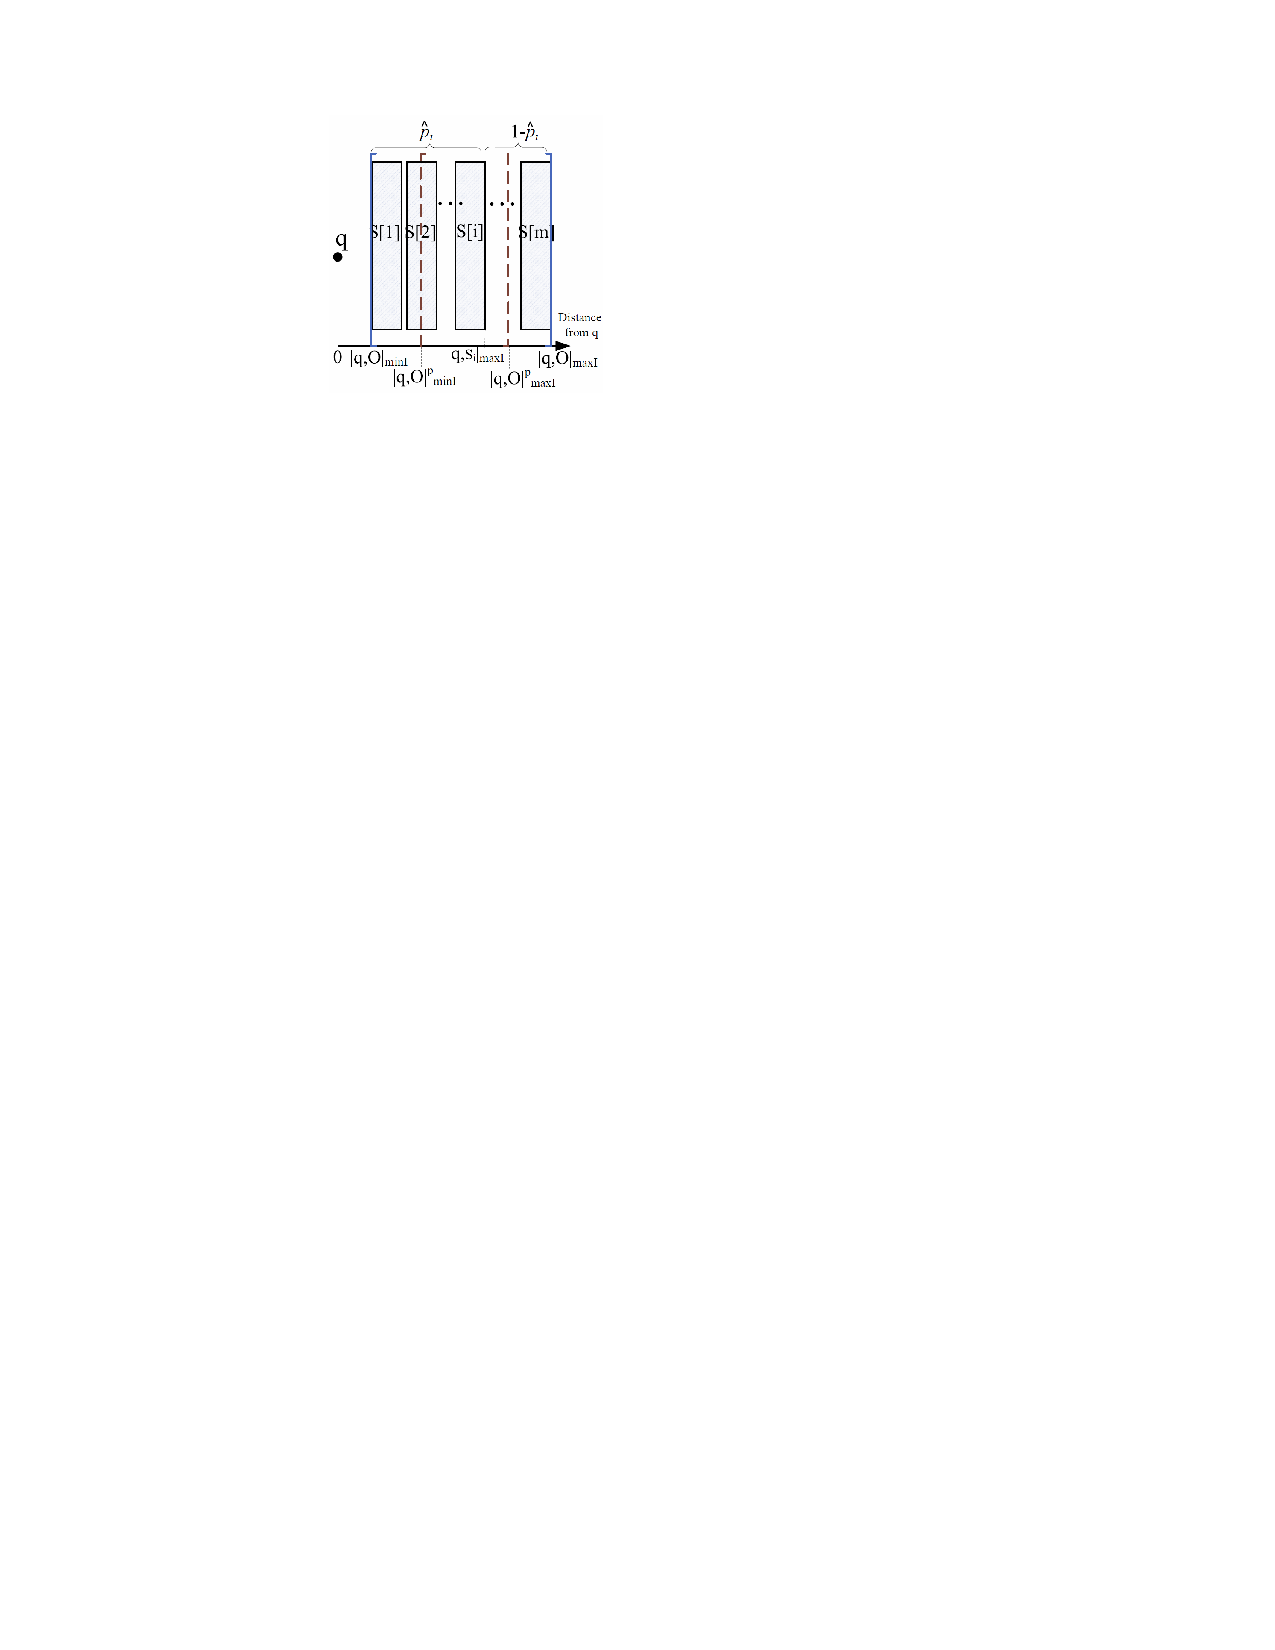
\includegraphics[width=\columnwidth]{figures/2-6/2-6-6.pdf}
  \end{figure}

  \column{0.7\textwidth}
  \begin{lemma}[Markov Lower Bounds]
    Suppose object $O$ overlaps with $m$ partitions $(O = \cup_{i=1}^{m}S[i])$, and $S[i]$s are sorted according to the minimum distance to a given point $q$. Use $\widehat{p_i}$ to denote $\sum_{j=1}^{i}p_i$. As $S[i]$ and $S[j]$ do not overlap, using \emph{Markov Inequality}, we have:
    \begin{equation*}
      E(|q, O|_I) \geq |q,S[i]|_{maxI} \cdot (1 - \widehat{p_i})
    \end{equation*}
  \end{lemma}

\end{columns}

\end{frame}

%------------------------------------------------

\begin{frame}
\frametitle{Bounds for Indoor Distances}

\conceptbf{Indoor Probabilistic ULBounds}

\vspace{10pt}
\begin{columns}[c]

  \column{0.3\textwidth}
  \begin{figure}[tb]
    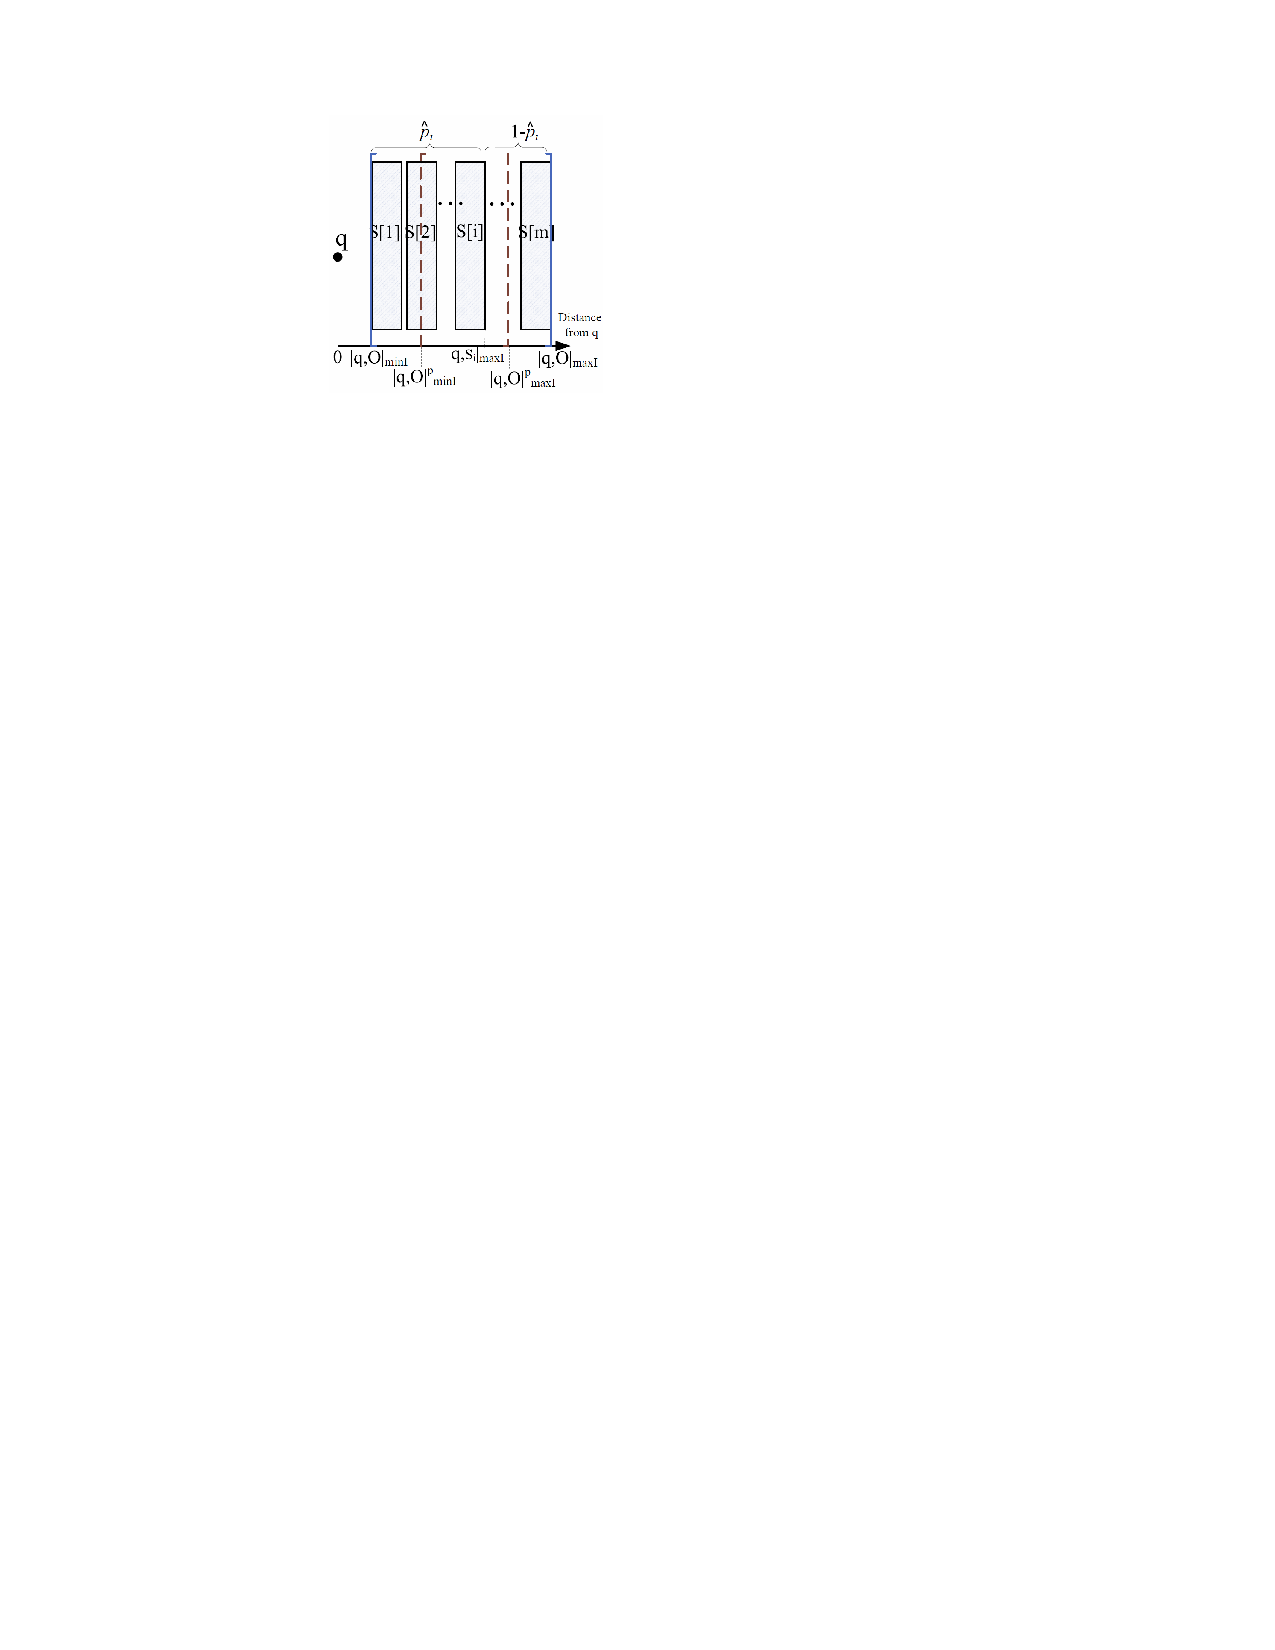
\includegraphics[width=\columnwidth]{figures/2-6/2-6-6.pdf}
  \end{figure}

  \column{0.7\textwidth}
  \begin{lemma}[Probabilistic ULBounds]
  \begin{equation*}
  \begin{split}
      & |q,S[i]|_{maxI} \cdot (1 - \widehat{p_i}) + |q, O|_{minI} \cdot \widehat{p_i} \\
      & \leq E(|q, O|_I) \leq \\
      & |q, O|_{maxI} \cdot (1 - \widehat{p_i}) + |q,S[i]|_{maxI} \cdot \widehat{p_i}
  \end{split}
  \end{equation*}
  \ssize{
  \textbf{Proof:} $ E(|q, O|_I)  = E(|q, \cup_{j \leq i}S[j]|_I) \cdot \widehat{p_i} +$\\
  $ E(|q, \cup_{k > i}S[k]|_I) \cdot (1 - \widehat{p_i})$. Since $|q,S[i]|_{maxI} \geq E(|q, \cup_{j \leq i}S[j]|_I) \geq |q,O|_{minI}$, and $|q,O|_{maxI} \geq E(|q, \cup_{k > i}S[k]|_I) \geq |q,O|_{minI}$, by substitution, the lemma is proved.
  }
  \end{lemma}

\end{columns}

\end{frame}

%------------------------------------------------

\begin{frame}
\frametitle{Summary}

use \emph{topological ULBounds} for the case that an object overlaps with a single partition; \\~\\

use \emph{probabilistic ULBounds} for the case that an object overlaps with multiple partitions.

\begin{figure}[tb]
  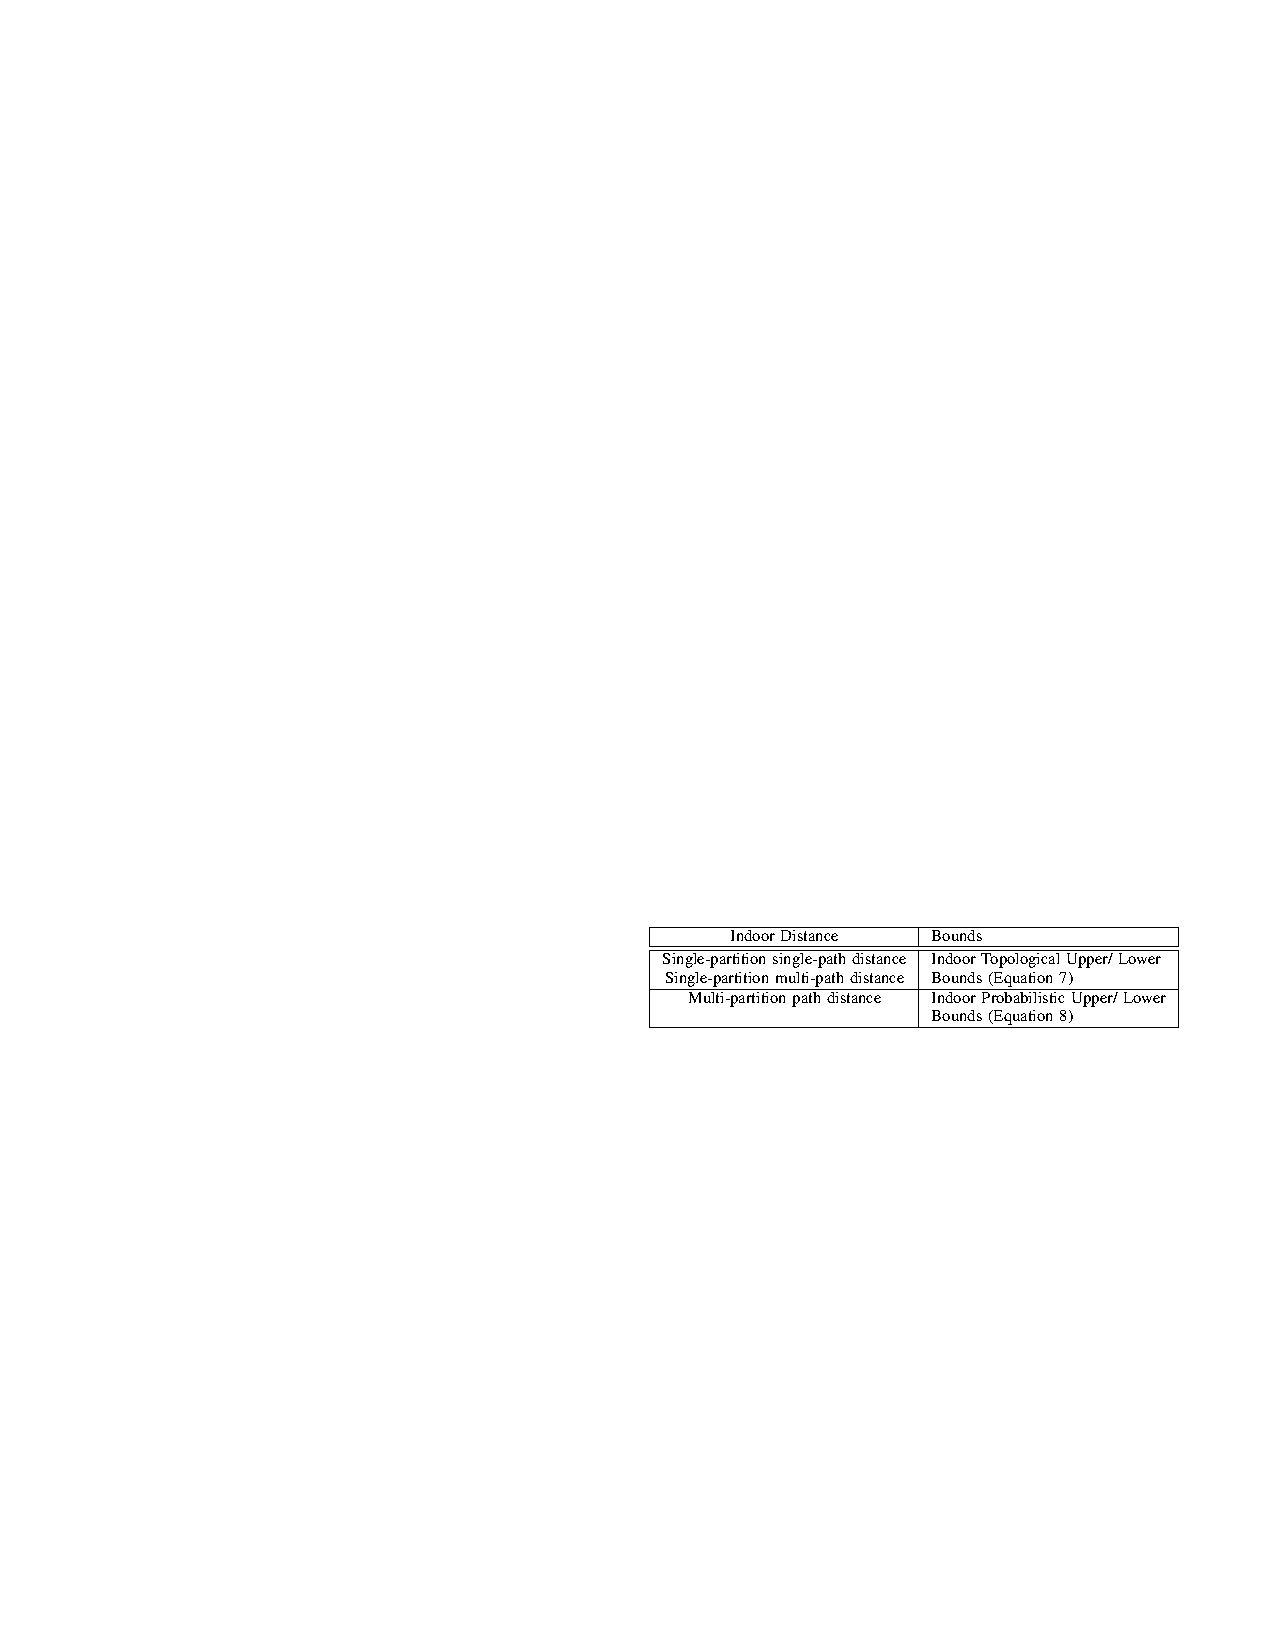
\includegraphics[width=0.7\columnwidth]{figures/2-6/2-6-7.pdf}
\end{figure}

with the Upper and Lower Bounds, as well as the approximate indoor distance, one can avoid computing shortest paths for all existential instances of an uncertain objects.

\end{frame}

%------------------------------------------------

\begin{frame}
\frametitle{Composite Index for Indoor Space}

\begin{columns}[c]

  \column{0.5\textwidth}
  \begin{figure}[tb]
    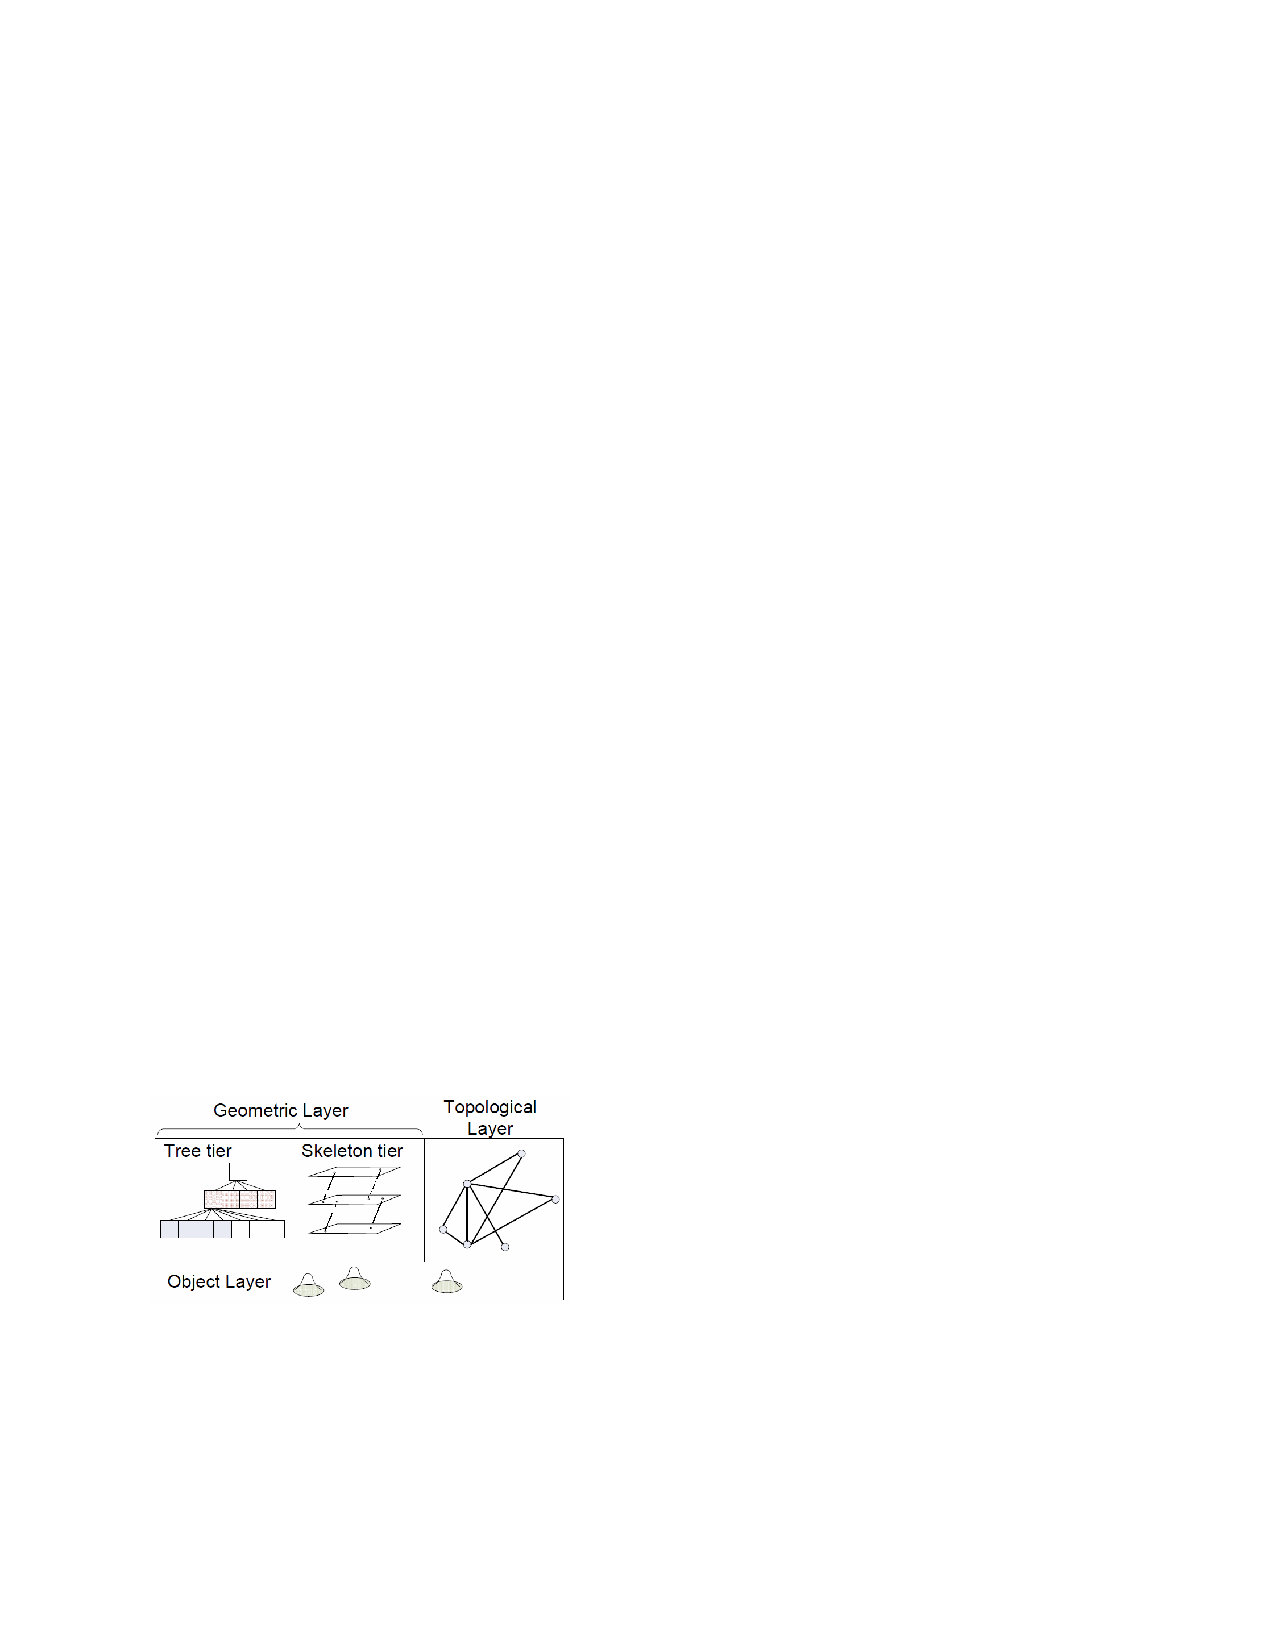
\includegraphics[width=\columnwidth]{figures/2-6/2-6-8.pdf}
  \end{figure}

  \column{0.5\textwidth}
  \begin{fitemize}
    \item \conceptbf{geometric layer} consists of a tree structure that adapts the R$^*$-tree to index all partitions, as well as a skeleton tier that maintains a small number of distances between staircases.
    \item \conceptbf{topological layer} maintains the connectivity information between indoor partitions.
    \item \conceptbf{object layer} stores all indoor moving objects and is associated with the tree through partitions at its leaf level.
  \end{fitemize}

\end{columns}

\end{frame}

%------------------------------------------------

\begin{frame}
\frametitle{Composite Index: Overview}

\begin{figure}[tb]
  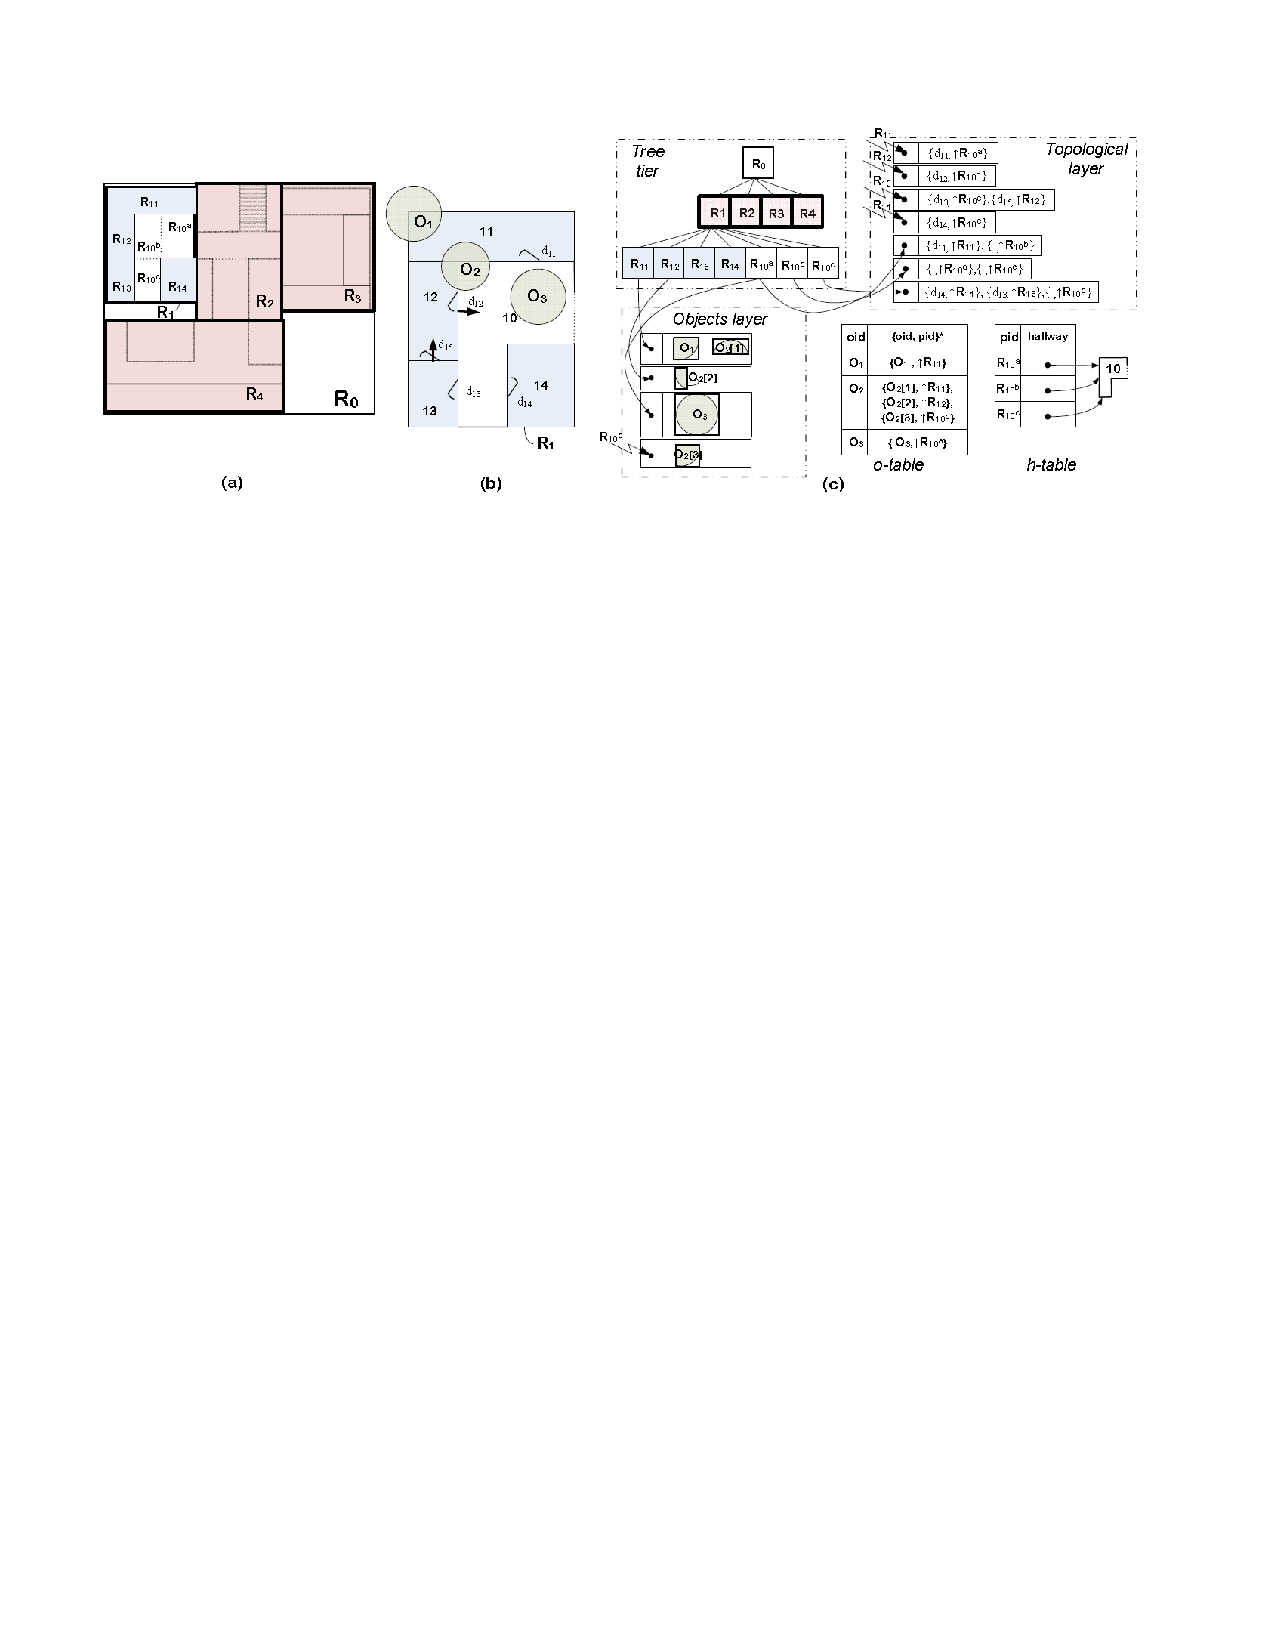
\includegraphics[width=\columnwidth]{figures/2-6/2-6-9.pdf}
\end{figure}

\end{frame}

%------------------------------------------------

\begin{frame}
\frametitle{Composite Index: Tree Tier}

\begin{fitemize}
  \item instead of 3D $Minimum Bounding Rectangle$, when creating the tree, set the vertical length for one partition to 1 centimeter. Two advantage: 1) reduce the distance calculation workload; 2) makes the distance reflected in the tree more accurate without the disturbance from the vertical dimension.
  \item the imbalanced partition are decomposed to small but regular region, each is called an \emph{index unit}.
  \item A hash table is used to map such an index unit to its original indoor partition.
\end{fitemize}

\vspace{-10pt}
\begin{figure}[tb]
  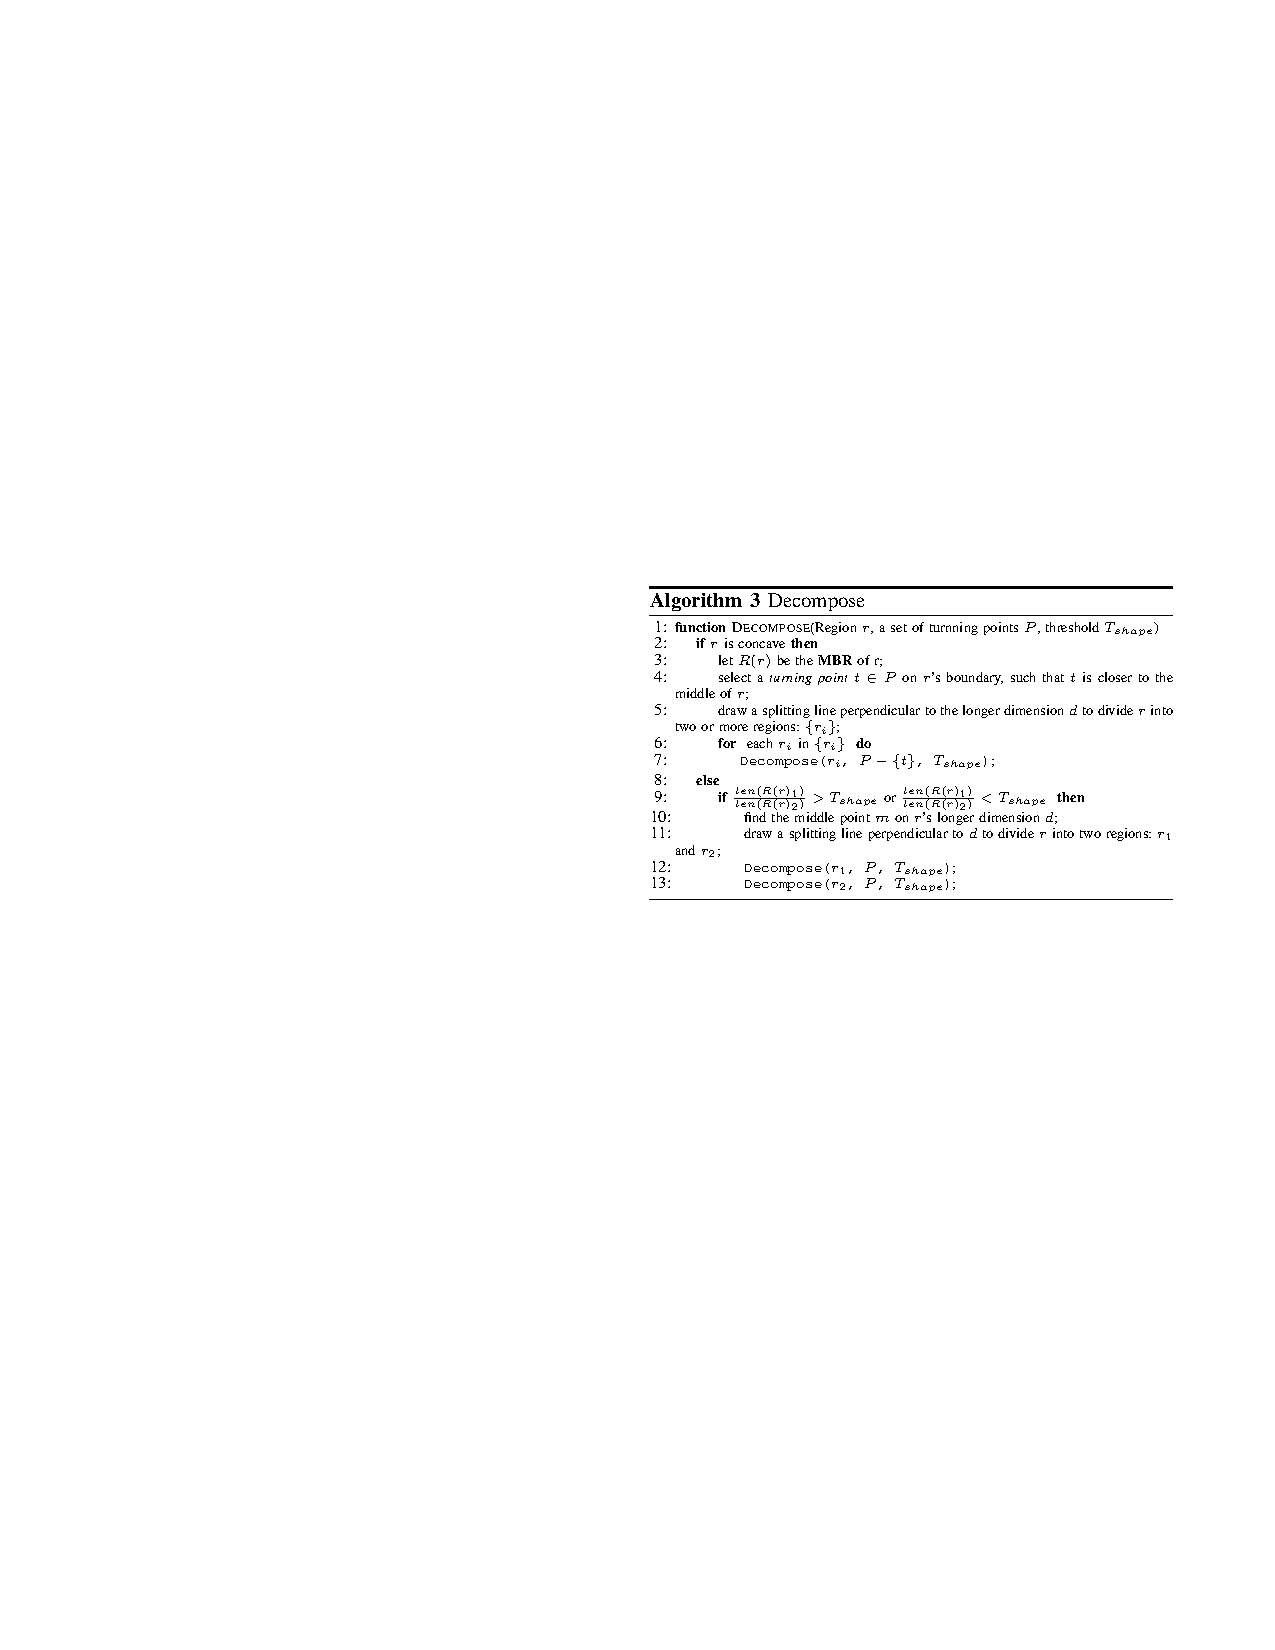
\includegraphics[width=0.55\columnwidth]{figures/2-6/2-6-10.pdf}
\end{figure}

\end{frame}

%------------------------------------------------

\begin{frame}
\frametitle{Composite Index: Object Tier}

A hash table $o-table$

\begin{equation*}
  o-table : \{ O \} \rightarrow 2^{\{index~unit\}}
\end{equation*}

$o-table$ maps an object to all the index units it overlaps, and it is tightly tie up with the tree tier.\\~\\

When an object update occurs, $o-table$ needs to be updated accordingly.

\end{frame}

%------------------------------------------------

\begin{frame}
\frametitle{Composite Index: Topological Tier}

This layer maintains the connectivity between partitions. Each leaf node stores a (sub)partition.\\~\\

For accessibility, the doors belonging to the partitions are also stored, as well as the the links to accessible partitions through each door.

\end{frame}

%------------------------------------------------

\begin{frame}
\frametitle{Composite Index: Skeleton Tier}

Skeleton Tier is a graph, each staircase entrance is captured as a graph node, and an edge connects two nodes if their entrances are on the same floor or their entrances belong to the same staircase.\\~\\

The weight of an edge is the indoor distance between the two staircase entrances.

\vspace{-10pt}
\begin{columns}[c]

  \column{0.4\textwidth}
  \begin{figure}[tb]
    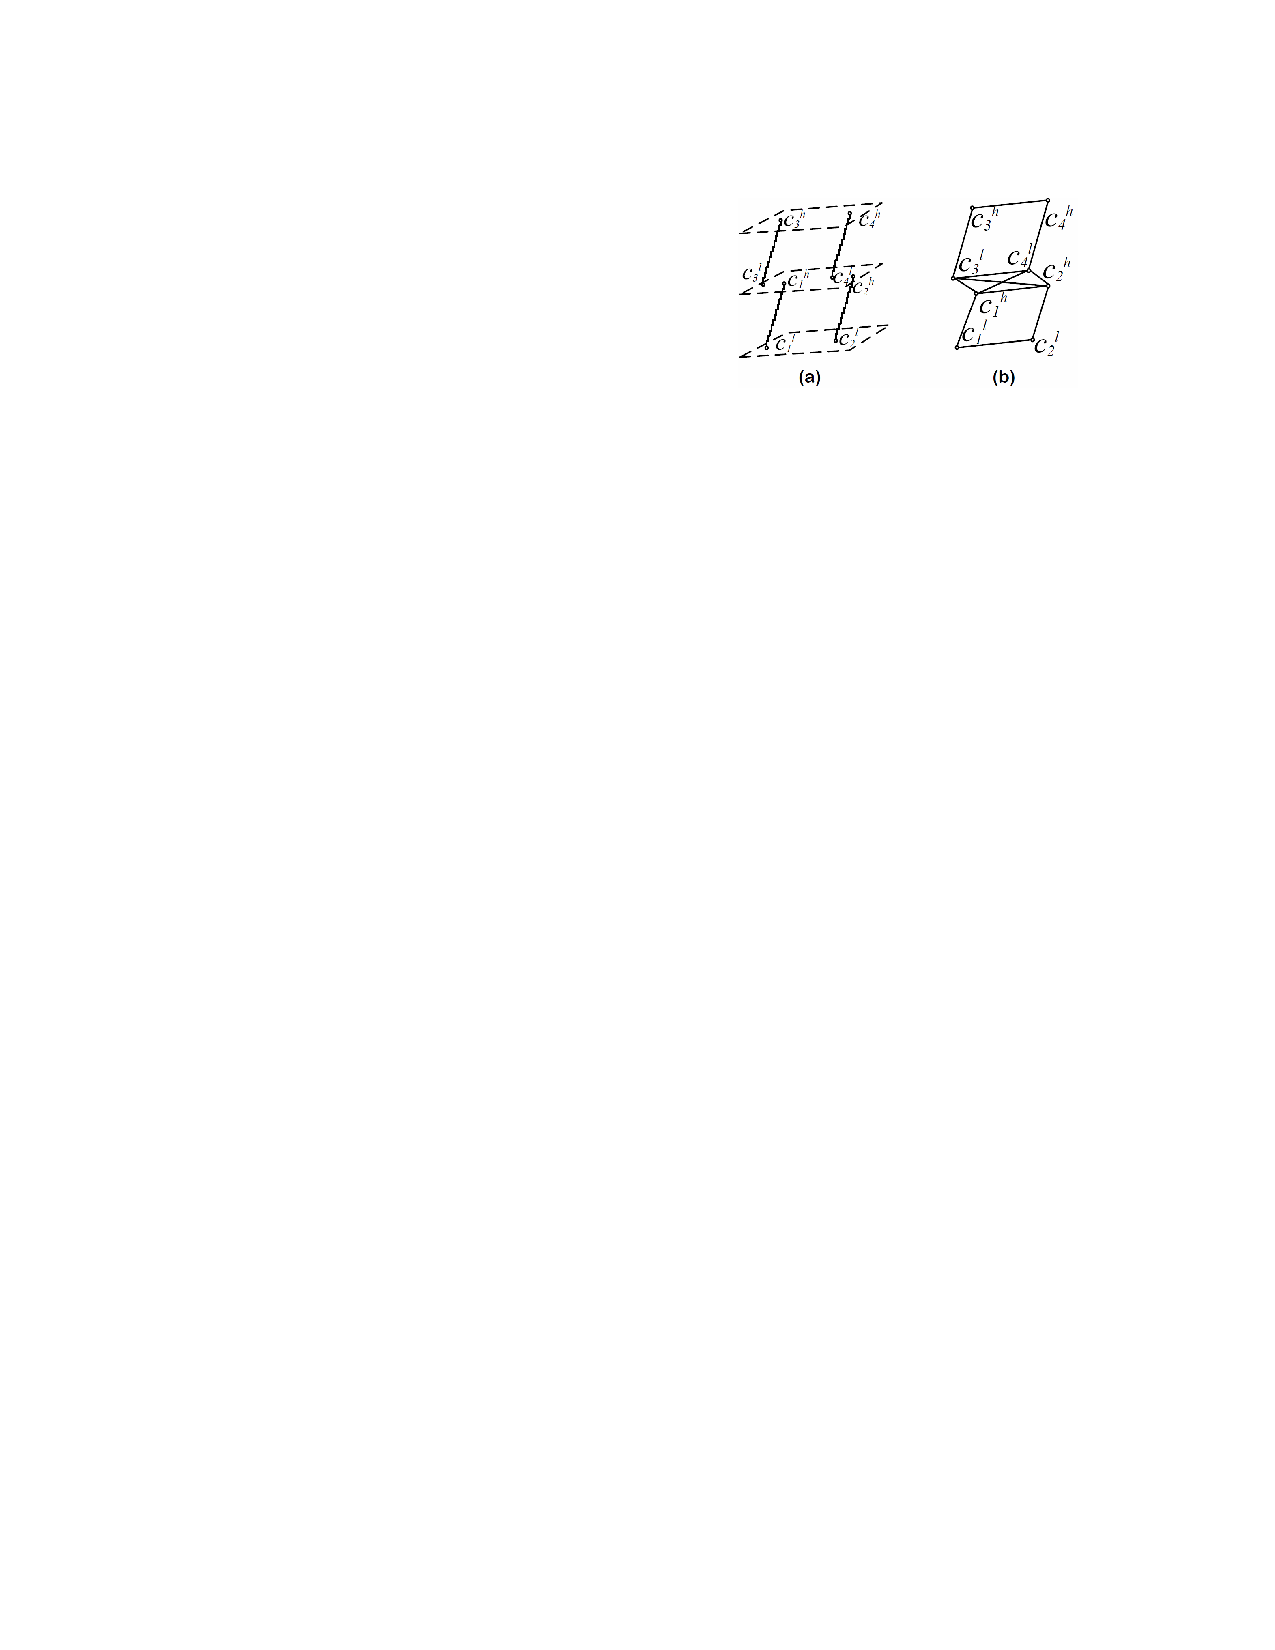
\includegraphics[width=\columnwidth]{figures/2-6/2-6-11.pdf}
  \end{figure}

  \column{0.6\textwidth}
  \ssize{
  \begin{definition}[staircase distance matrix $M_{s2s}$]
    \begin{sitemize}
      \item $M_{s2s}[s_i,s_i] = 0$;
      \item $M_{s2s}[s_i,s_j] = |s_i, s_j|_E$ if $s_i$ and $s_j$ are on the same floor;
      \item if $s_i$ and $s_j$ are of a same staircase, $M_{s2s}[s_i,s_j]$ is the shortest distance from $s_i$ to $s_j$ within that staircase;
      \item $M_{s2s}[s_i,s_j]$ is calculated as the shortest path distance from $s_i$ to $s_j$ in the skeleton layer for other cases.
    \end{sitemize}
  \end{definition}
  }

\end{columns}

\end{frame}

%------------------------------------------------

\begin{frame}
\frametitle{Skeleton Distance}

\textrm{Let $q$ be a fixed indoor point, $q.f$ the floor of $q$, and $S(q.f)$ all the staircases on floor $q.f$.}

\vspace{10pt}
\begin{definition}[Skeleton Distance]
  Given two points $p$ and $q$, their skeleton distance $|q,p|_K = |q,p|_E$ if they are on the same floor; otherwise, $|q,p|_K = \min_{s_q \in S(q.f), s_p \in S(p.f)}(|q,s_q|_E + M_{s2s}[s_q,s_p] + |s_p, p|_E)$.
\end{definition}

\vspace{10pt}
Define the skeleton distance as the alternative \emph{Geometric Distance}.

\end{frame}

%------------------------------------------------

\begin{frame}
\frametitle{Indoor Distance Bounds in the Geometric Layer}

\begin{lemma}[Geometric Lower Bound Property]
  Given two points $p$ and $q$, their skeleton distance lower bounds their indoor distance, i.e., $|q,p|_K \leq |q,p|_I$.\\~\\
  \textbf{Proof:}~If $q$ and $p$ are on the same floor, $|q,p|_K = |q,p|_E \leq |q,p|_I$. Otherwise, suppose $s_{q}^{*} \in S(q.f)$ and $s_{p}^{*} \in S(p.f)$ are on the shortest path from $q$ to $p$, denoted by $q \overset{*s_{q}^{*}*s_{p}^{*}}{\rightarrow} p$. Since $|q,p|_K = \min_{s_q \in S(q.f), s_p \in S(p.f)}(|q,s_q|_E + M_{s2s}[s_q,s_p] + |s_p, p|_E) \leq |q,s_{q}^{*}|_E + M_{s2s}[s_{q}^{*},s_{p}^{*}] + |s_{p}^{*}, p|_E = |q,p|_I$, the lemma is proved.
\end{lemma}

\end{frame}

%------------------------------------------------

\begin{frame}
\frametitle{Indoor Distance Bounds in the Geometric Layer}

Consider an entity $e$ that is either an object or an $ind$R-tree node. If $e$ spans multiple floors, we use interval $[e.lf,e.uf]$ to represent all those floors. Note those floors must be consecutive. We define the minimum skeleton distance $|q,e|_{minK}$:

\begin{figure}[tb]
  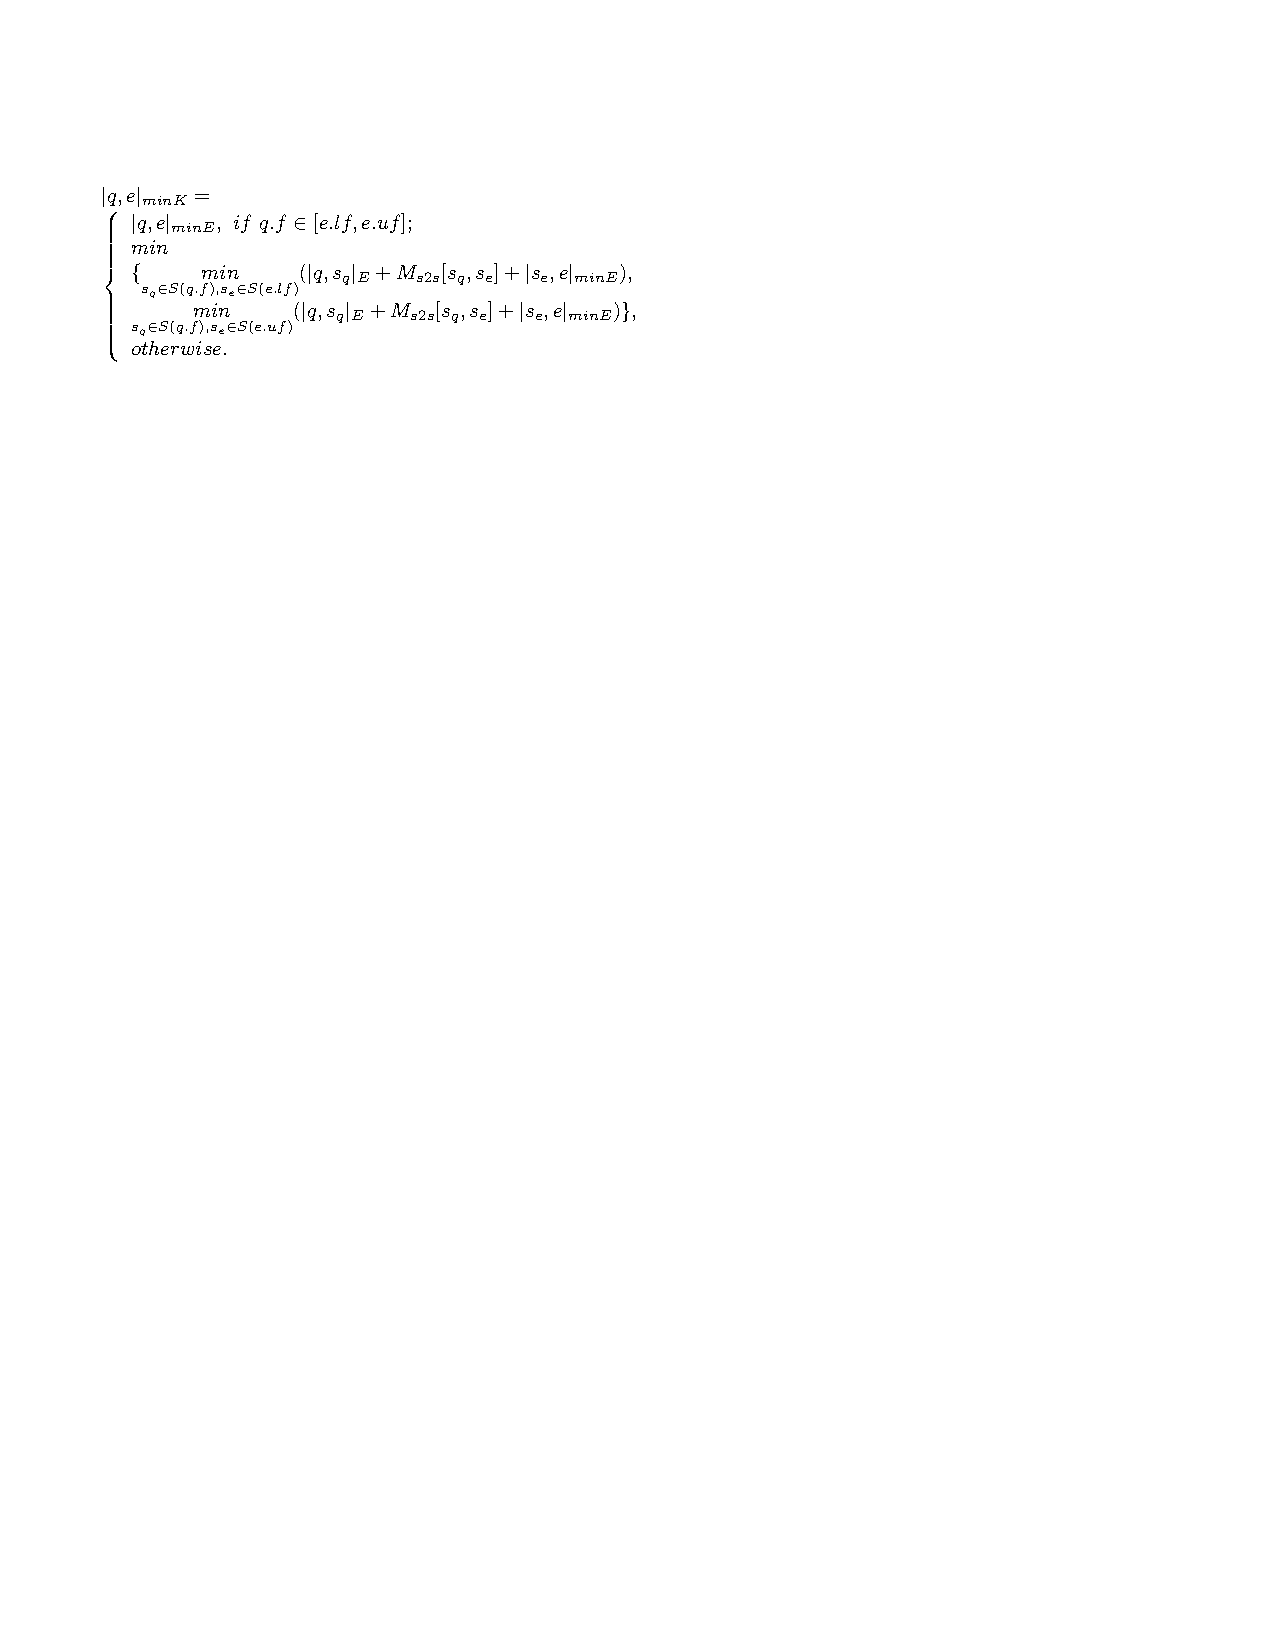
\includegraphics[width=0.7\columnwidth]{figures/2-6/2-6-12.pdf}
\end{figure}

With $|q,e|_{minK}$, one can constrain the search via the $ind$R-tree to a much smaller range compared to if use the Euclidean distance bounds.

\end{frame}

%------------------------------------------------

\begin{frame}
\frametitle{Dynamic Operations on the Topological Layer}

\textbf{Insertion.}~\textrm{When the topological change leads to a new indoor partition $P$, $P$(or its sub-partitions due to decomposition) is inserted into the $ind$R-tree, its leaf node is connected to the adjacent partitions, and the $h-table$ is updated if a decomposition is invovled.}\\~\\

\textbf{Deletion.}~\textrm{From the $ind$R-tree to remove a partition $P$ to be deleted, the links involving $P$ are removed from the adjacent partitions, and $P$'s entry in the $h-table$ is deleted if $P$ is a decomposed sub-partition.}

\end{frame}

%------------------------------------------------

\begin{frame}
\frametitle{Dynamic Operations on the Object Layer}

\textbf{Insertion.}~\textrm{To insert an object $O$, search the $ind$R-tree to find the leaf nodes $\{ P_i \}$ that overlap with $O$'s uncertainty region. Also insert a new entry to $o-table$.}\\~\\

\textbf{Deletion.}~\textrm{To delete an object $O$, use the $o-table$ to find the $ind$R-tree leaf nodes $\{ P_i \}$ that overlap with $O$'s uncertainty region. For each $P_i$, $O$ is removed from its associated bucket. Also the entry for $O$ is deleted from the $o-table$.}

\end{frame}

%------------------------------------------------

\begin{frame}
\frametitle{Query Semantics}

\begin{definition}[Indoor Range Query, iRQ]
  Given a query point $q \in \mathbb{I}$ and a distance value $r$, the \emph{iRQ} returns objects whose indoor distances are smaller than $r$. Formally, $iRQ_{q,r}(\mathbb{O}) = \{ O | |q,O|_I \leq r, O \in \mathbb{O}\}$.
\end{definition}

\begin{definition}[Indoor $k$ Nearest Neighbor Query, ikNNQ]
  Given a query point $q \in \mathbb{I}$ and a parameter $k$, the \emph{ikNNQ} returns $k$ objects whose indoor distances to $q$ are the smallest among all objects. Formally, $ikNN_{q,k}(\mathbb{O}) = \{ O | O \in \mathbb{O}\}$, where $|ikNN_{q,k}(\mathbb{O})| = k, \forall O_i \in ikNN_{q,k}(\mathbb{O}), \forall O_j \in \mathbb{O} \setminus ikNN_{q,k}(\mathbb{O}), |q,O_i|_I \leq |q,O_j|_I$.
\end{definition}

\end{frame}

%------------------------------------------------

\begin{frame}
\frametitle{Efficient Query Evaluation}

\begin{enumerate}
  \fsize{
  \item \conceptbf{Filtering Phase} locates the source partition that contains the query point and retrieves condidate partitions as well as candidate objects.
  \item \conceptbf{Subgraph Phase} constructs a subgraph based on candidate partitions, and uses the doors of the source partition as sources to compute the shortest indoor paths that are to be used in the subsequent two phases.
  \item \conceptbf{Prunning Phase}, upper/lower distance bounds for objects are calculated to further reduce the number of candidate objects.
  \item \conceptbf{Refinement Phase}, the indoor distances for the remaining objects are computed and the qualifying objects are returned as the query results.
  }
\end{enumerate}

\end{frame}

%------------------------------------------------

\begin{frame}
\frametitle{Indoor Range Query}

\begin{columns}[c]

  \column{0.2\textwidth}
  \begin{figure}[tb]
    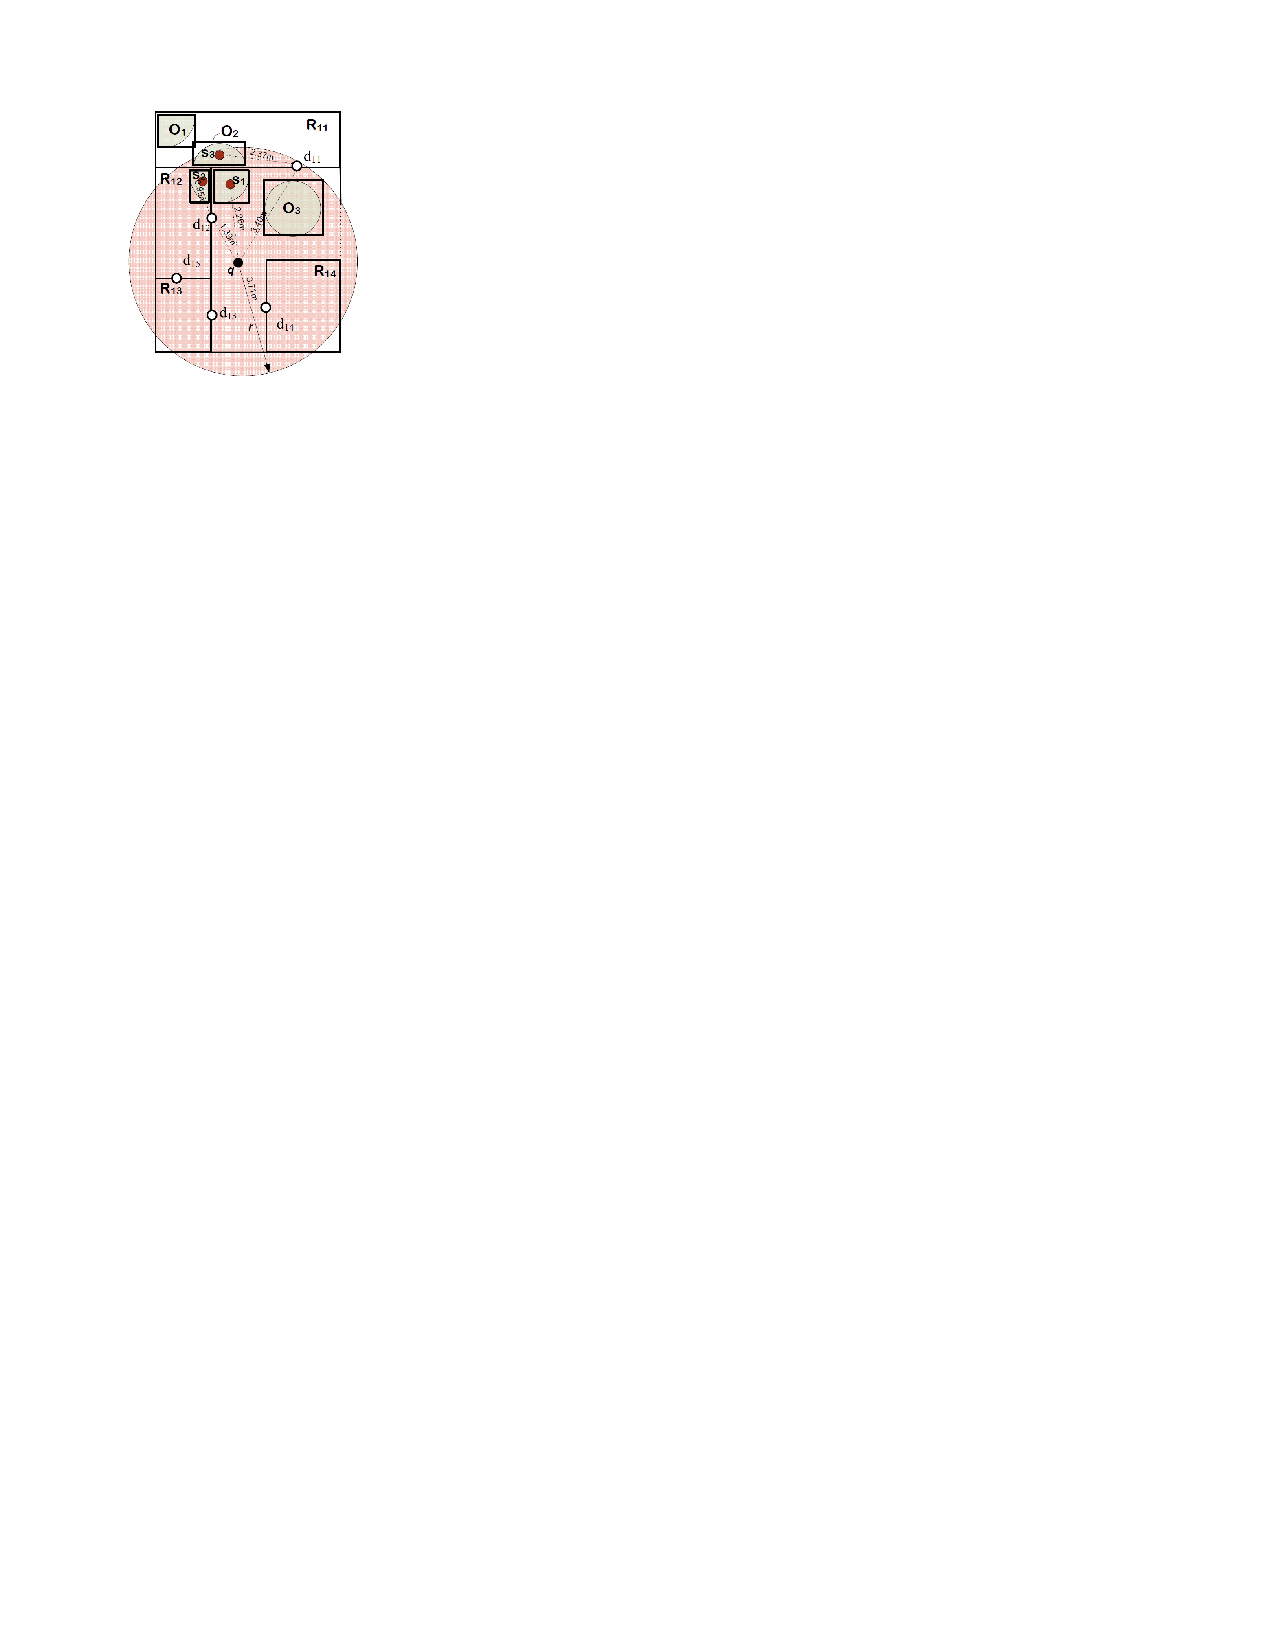
\includegraphics[width=\columnwidth]{figures/2-6/2-6-13.pdf}
  \end{figure}


  \column{0.8\textwidth}
  \begin{example}
    \ssize{
    The circle $\bigodot(q,r)$ is the query region represented in the Euclidean space. Object $O_1$ is pruned away in filtering phase, since $|q, O_1|_{minE} > r$. After deriving the upper/lower bounds for the remaining objects in the pruning phase, $O_3$ is qualified. For the undetermined object $O_2$, the exact indoor distance is calculated and compared to $r$.
    }
  \end{example}

\end{columns}

\begin{columns}[c]

  \column{0.4\textwidth}
  \begin{figure}[tb]
    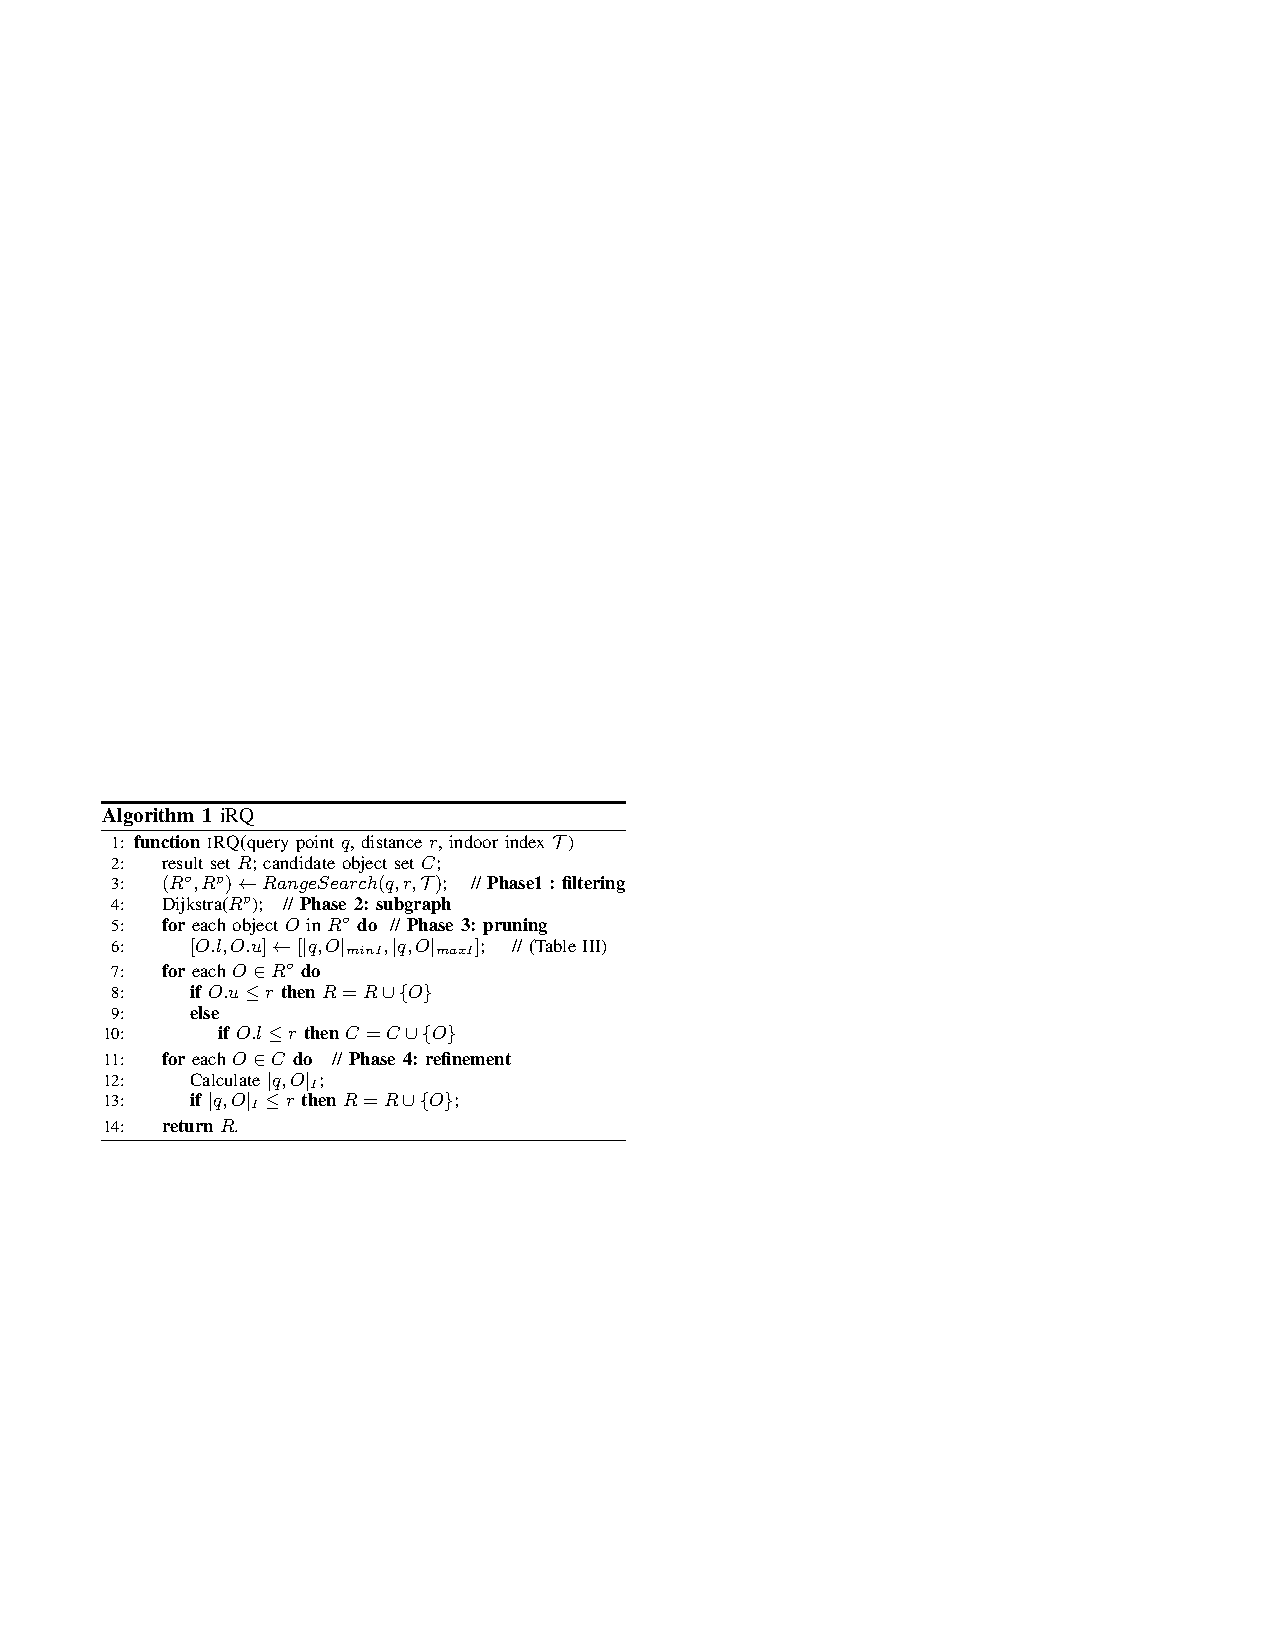
\includegraphics[width=\columnwidth]{figures/2-6/2-6-14.pdf}
  \end{figure}

  \column{0.6\textwidth}
  \begin{sitemize}
    \item in the filtering, iRQ calls $RangeSearch$ to search the geometric layer.
    \item lines 5--10: iRQ makes use of the topological upper/lower bounds to approximate indoor distances and compare them to $r$.
    \item lines 11--13: the exact indoor distances are only computed for those objects whose bounds cover $r$.
  \end{sitemize}

\end{columns}

\end{frame}

%------------------------------------------------

\begin{frame}
\frametitle{Indoor $k$ Nearest Neighbor Query}

\begin{columns}[c]

  \column{0.16\textwidth}
  \begin{figure}[tb]
    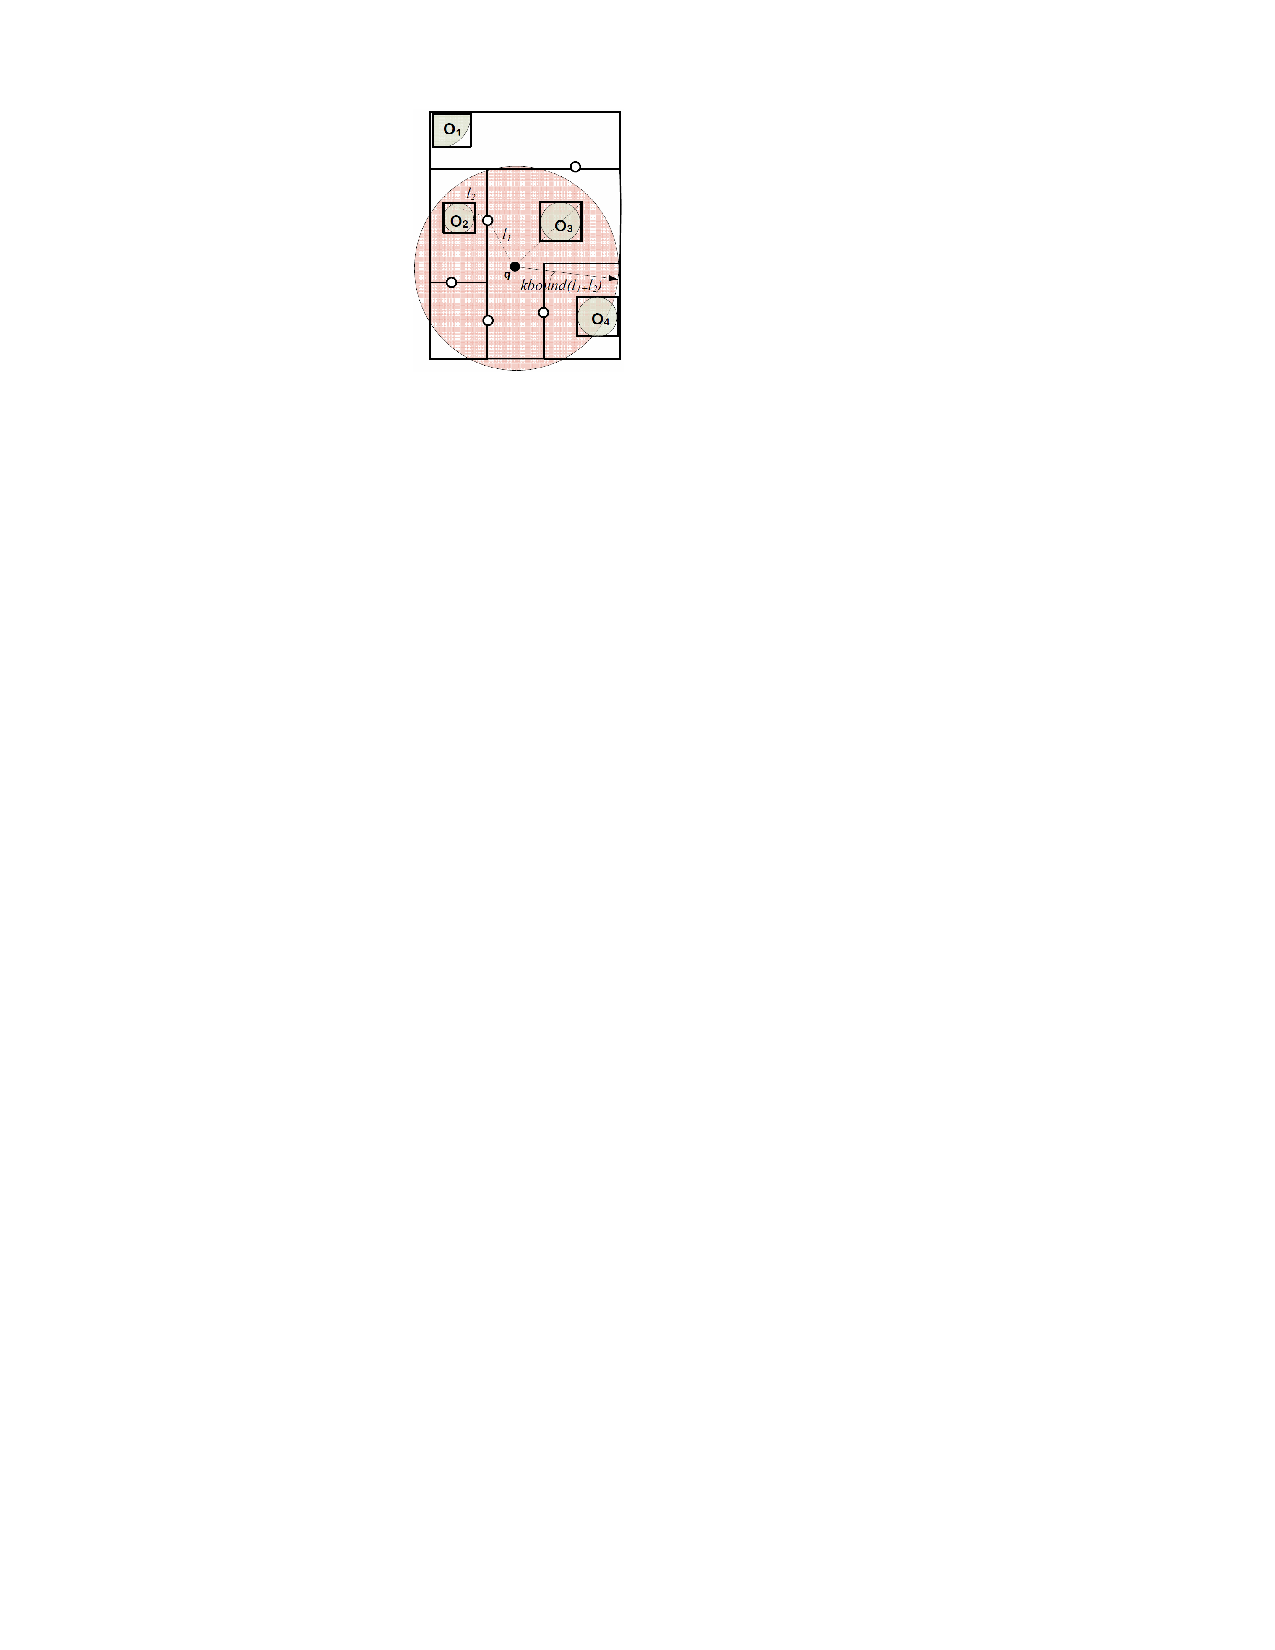
\includegraphics[width=\columnwidth]{figures/2-6/2-6-15.pdf}
  \end{figure}


  \column{0.84\textwidth}
  \begin{example}
    \ssize{
    $kSeedsSelection$ finds $O_2$ and $O_3$ as seeds. Because $O_2$'s topological looser upper bound is longer, it is chosen as the kbound. Through the range search, $O_1$ is excluded since $|q,O_1|_K > kbound$.
    }
  \end{example}

\end{columns}

\begin{columns}[c]

  \column{0.35\textwidth}
  \begin{figure}[tb]
    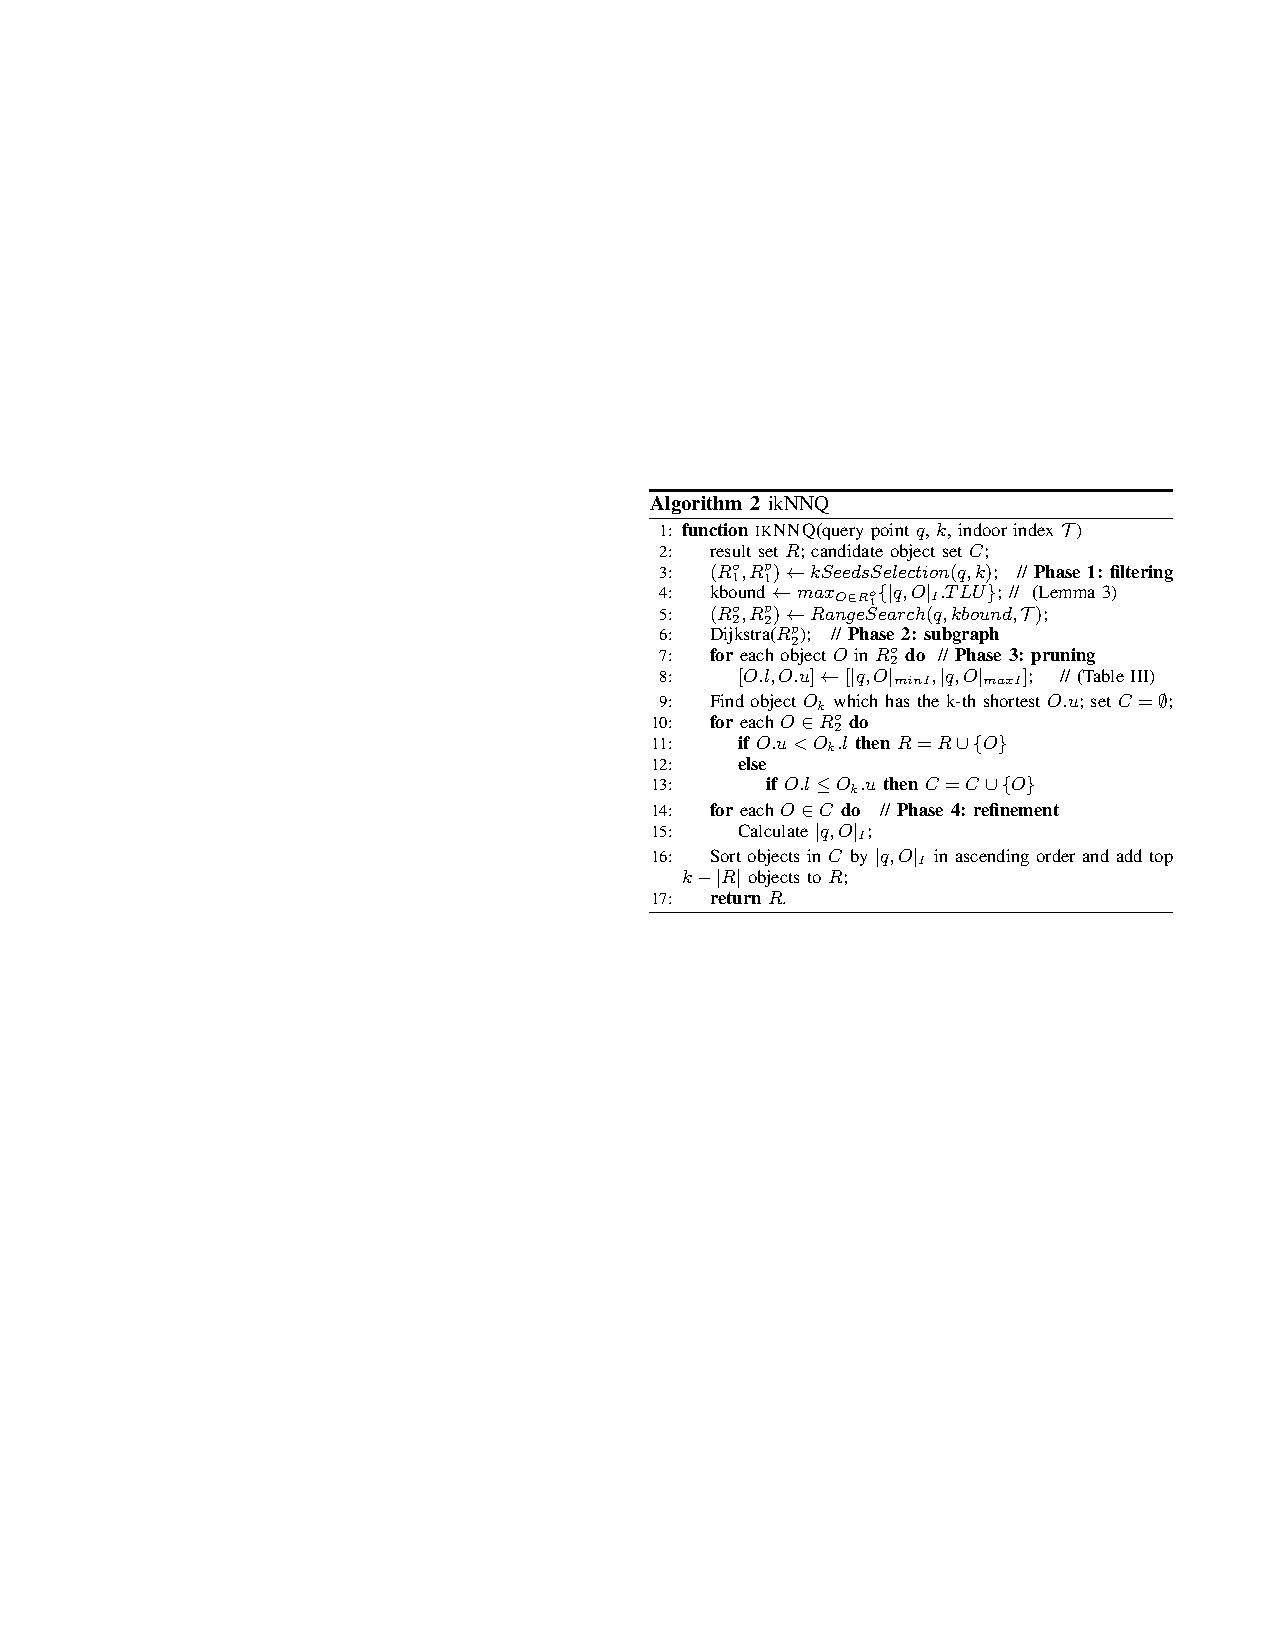
\includegraphics[width=\columnwidth]{figures/2-6/2-6-16.pdf}
  \end{figure}

  \column{0.65\textwidth}
  \begin{sitemize}
    \item in the filtering, ikNNQ calls $kSeedsSelection$ to return an object $R_1^o$ and a partition set $R_1^p$.
    \item $R_1^o$ contains $k$ objects taht are in query point $q$'s partition or in the closet adjacent partitions. $R_1^p$ is the set of all those involved partition.
    \item ikNNQ derives \emph{Topological Looser Upper Bounds} for the $k$ objects and choose the longest one as $kounds = \max_{seed_i \in R_1^o}\{ |q,seed_i|_I.TLU \}$.
    \item Line 4: a range search $\bigodot(q,kound)$ is done on the tree tier.
  \end{sitemize}

\end{columns}

\end{frame}

%------------------------------------------------

\begin{frame}
  \frametitle{Research Directions}

  \begin{itemize}
  	\item it is of interest to study other query types using the distance bounds and the composite index proposed in this paper.
    \item it is useful to estimate the selectivity for indoor distance aware queries and make use of it in further optimizing queries over uncetain object.
    \item it is of benificial to reuse computational efforts on indoor distances when multiple, related queries are issued within a short period of time.
  \end{itemize}

\end{frame}


%------------------------------------------------
\section{3. Indoor Data Cleansing} % Sections can be created in order to organize your presentation into discrete blocks, all sections and subsections are automatically printed in the table of contents as an overview of the talk
%------------------------------------------------

%------------------------------------------------
\section{4. Indoor Movement Analysis} % Sections can be created in order to organize your presentation into discrete blocks, all sections and subsections are automatically printed in the table of contents as an overview of the talk
%------------------------------------------------

%------------------------------------------------
\section{5. Appendix} % Sections can be created in order to organize your presentation into discrete blocks, all sections and subsections are automatically printed in the table of contents as an overview of the talk
%------------------------------------------------

\begin{frame}
\frametitle{References}

\begin{thebibliography}{99} % Beamer does not support BibTeX so references must be inserted manually as below
\fsize{
\bibitem{DBLP:conf/gis/Worboys11}
M.~F. Worboys.
\newblock Modeling indoor space.
\newblock In {\em {ISA}}, pp. 1--6, 2011.

\bibitem{DBLP:conf/mdm/JensenLY09}
C.~S. Jensen, H.~Lu, and B.~Yang.
\newblock Graph model based indoor tracking.
\newblock In {\em {MDM}}, pp. 122--131, 2009.

\bibitem{DBLP:conf/cikm/YangLJ09}
B.~Yang, H.~Lu, and C.~S. Jensen.
\newblock Scalable continuous range monitoring of moving objects in symbolic
  indoor space.
\newblock In {\em CIKM}, pp. 671--680, 2009.

\bibitem{DBLP:conf/edbt/YangLJ10}
B.~Yang, H.~Lu, and C.~S. Jensen.
\newblock Probabilistic threshold k nearest neighbor queries over moving
  objects in symbolic indoor space.
\newblock In {\em EDBT}, pp. 335--346, 2010.
}
\end{thebibliography}

\end{frame}

%------------------------------------------------

\begin{frame}
\frametitle{References}

\begin{thebibliography}{99} % Beamer does not support BibTeX so references must be inserted manually as below
\fsize{

\bibitem{DBLP:conf/icde/LuYCJ11}
H.~Lu, B.~Yang, and C.~S. Jensen.
\newblock Spatio-temporal Joins on Symbolic Indoor Tracking Data.
\newblock In {\em {ICDE}}, pp. 816--827, 2011.

\bibitem{DBLP:conf/icde/LuCJ12}
H.~Lu, X.~Cao, and C.~S. Jensen.
\newblock A foundation for efficient indoor distance-aware query processing.
\newblock In {\em ICDE}, pp. 438--449, 2012.

\bibitem{DBLP:conf/icde/XieLP13}
X.~Xie, H.~Lu, and T.~B. Pedersen.
\newblock Efficient distance-aware query evaluation on indoor moving objects.
\newblock In {\em ICDE}, pp. 434--445, 2013.

\bibitem{hightower2001location}
Hightower, Jeffrey and Borriello, Gaetano.
\newblock Location systems for ubiquitous computing.
\newblock In {\em Journal of Computer}, pp. 7--66, 2001

}
\end{thebibliography}

\end{frame}



%----------------------------------------------------------------------------------------

\begin{frame}
\Huge{\centerline{The End. Thanks :)}}
\end{frame}

%----------------------------------------------------------------------------------------

\end{document}
